\documentclass[a4paper,10pt]{article}%
\input{commands.tex}%

\author{Peter Bonventre, Lu\'is A. Pereira}%
\title{Genuine equivariant operads}%

\usepackage[hidelinks]{hyperref}
\hypersetup{
%  colorlinks,
  linktoc=page
}

\usepackage{showkeys}

\usepackage{stmaryrd}

\usepackage{geometry}

\usepackage{tikz}%
\tikzset{%
  treenode/.style = {shape=rectangle, rounded corners,%
                     draw, align=center,%
                     top color=white, bottom color=blue!20},%
  root/.style     = {treenode, font=\Large, bottom color=red!30},%
  env/.style      = {treenode, font=\ttfamily\normalsize},%
  dummy/.style    = {circle,draw,inner sep=0pt,minimum size=2mm}%
}%

\usetikzlibrary[decorations.pathreplacing]

\begin{document}	\maketitle%


\abstract{We build new algebraic structures, which we call genuine equivariant operads, which can be thought of as a hybrid between equivariant operads and coefficient systems.
We then prove an Elmendorf type theorem stating that equivariant operads, with their graph model structure, are equivalent to genuine equivariant operads with their projective model structure.

As an application, we build explicit models for the $N_{\infty}$-operads of Blumberg and Hill.
}

\tableofcontents

\section{Introduction}

No content yet.



\section{Basic definitions}

In this section we recall some definitions that will be used throughout.



Recall that for a diagram category $\mathcal{D}$ and functor $\mathcal{I}_{\bullet}$
\begin{equation}
\begin{tikzcd}[row sep = 0.2em]
	\mathcal{D} \ar{r}{\mathcal{I}_{\bullet}} & \mathsf{Cat} \\
	d \ar[mapsto]{r} & \mathcal{I}_d
\end{tikzcd}
\end{equation}
the (covariant) Grothendieck construction 
$\mathcal{D} \ltimes \mathcal{I}_{\bullet}$
has objects pairs $(d,i)$ with $d \in \mathcal{D}$,
 $i \in \mathcal{I}_d$ and 
arrows $(d,i) \to (d',i')$ given by pairs
\[(f\colon d \to d', g \colon f_{\**}(i) \to i'),\]
where $f_{\**}\colon \mathcal{I}_d \to \mathcal{I}_{d'}$ is a shorthand for the functor $\mathcal{I}_{\bullet}(f)$.


We now discuss a basic property of over and under categories that will be used in Section \ref{TRANSFSIMP SEC}.

Given $\mathcal{J},\C \in \mathsf{Cat}$ and $j \in \mathcal{J}$ we will let $\C^{ \downarrow j}$ denote the Grothendieck construction for the functor
\[
\begin{tikzcd}[row sep = 0.25em]
	\mathcal{J} \ar{r} & \mathsf{Cat} \\
	i \ar[mapsto]{r} & \C^{\mathcal{J}(i,j)}
\end{tikzcd}
\]
Explicitly, an object of $\C^{\downarrow j}$ is a pair
$\left(i,\mathcal{J}(i,j)\xrightarrow{\varphi} \C\right)$
and an arrow 
$(i,\varphi) \to (i',\varphi')$
is a pair
$(I \colon i \to i', 
\gamma \colon \varphi\circ I^{\**} \to \varphi')$.

	

\begin{lemma}\label{UNDERLEFTADJ LEM}
Let $\mathcal{J} \in \mathsf{Cat}$ be a small category and 
$j \in \mathcal{J}$. One then has adjunctions
\[
	(\minus \downarrow j) 
		\colon
	\mathsf{Cat}_{/\mathcal{J}}
		\rightleftarrows
	\mathsf{Cat}
		\colon
	(\minus)^{\downarrow j},
\qquad
	(j \downarrow \minus) 
		\colon
	\mathsf{Cat}_{/\mathcal{J}}
		\rightleftarrows
	\mathsf{Cat}
		\colon
	(\minus)^{j \downarrow}.
\]
\end{lemma}

\begin{proof}
Since $j \downarrow \mcI = (\mcI^{op} \downarrow j)^{op}$ by  defining $(\C^{j \downarrow}) = ((\C^{op})^{\downarrow j})^{op}$ one reduces to the leftmost adjuntion.

	Given $\mcI \xrightarrow{\pi} \mathcal{J}$ and $\C$ we will show that functors 
	$\mathcal{I} \downarrow j \xrightarrow{F} \C$
correspond to functors
	$\mathcal{I} \xrightarrow{G} \C^{\downarrow j}$ over $\mathcal{J}$.
	
	On objects, $F$ associates to each pair 
	$(i,J\colon \pi(i) \to j)$ an object $F(i,J)\in \C$. One thus sets $G(i)=(\pi(i), F(i,\minus))$ and these are clearly inverse processes.

	On arrows $F$ associates to 
	$(i,J' \circ \pi(I)) \xrightarrow{I} (i',J')$ an arrow
	$F(i,J' \circ \pi(I)) \xrightarrow{F(I)} F(i',J')$.
	One thus defines
\[
	G(I) = \left(
	\pi(i) \xrightarrow{\pi(I)} \pi(i'),
	F\left(i,(\minus)\circ \pi(i)\right)
		\xrightarrow{F(I)}
	F\left(i',\minus \right)
	\right)
\]
and again it is clear that these are inverse processes.
	Finally, the fact that the associativity and unit conditions for $F,G$ coincide is likewise clear.
\end{proof}







\section{Planar and tall maps}

\subsection{Planar structures}


Throughout we will work with trees possessing \textit{planar structures} or, more intuitively, trees embedded into the plane.

Our preferred model for trees will be that of broad posets first introduced by Weiss in \cite{We12} and further worked out by the second author in \cite{Pe16b}. We now define planar structures in this context.


\begin{definition}\label{PLANARIZE DEF}
	Let $T \in \Omega$ be a tree. A \textit{planar structure} of $T$ is an extension of the descendancy partial order $\leq_d$ to a total order $\leq_p$ such that: 
	\begin{itemize}
		\item \textit{Planar}: if $e \leq_p f$ and $e \nleq_d f$ then 
		$g \leq_d f$ implies $e \leq_p g$.
	\end{itemize} 
\end{definition}


\begin{example}
An example of a planar structure on a tree $T$ follows, with $\leq_r$ encoded by the number labels.
\begin{equation}\label{PLANAREX EQ}
	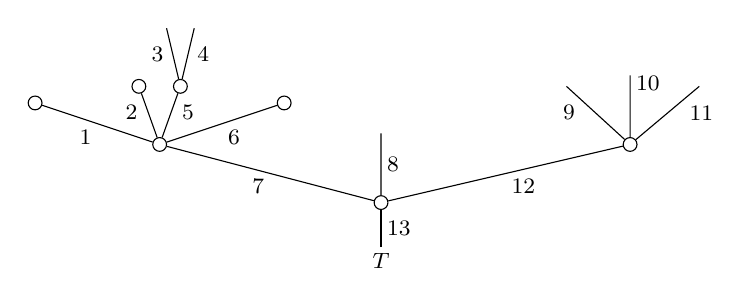
\begin{tikzpicture}[grow=up,auto,level distance=2.1em,
	every node/.style = {font=\footnotesize,inner sep=2pt},
	dummy/.style={circle,draw,inner sep=0pt,minimum size=1.75mm}]
		\node at (0,0) {$T$}
			child{node [dummy] {}
				child[sibling distance = 9em]{node [dummy] {}
					child[sibling distance = 2.5em]{
					edge from parent node [near end,swap] {$11$}}
					child[level distance=2.5em]{
					edge from parent node [very near end,swap] {$10$}}				
					child[sibling distance = 2.3em]{
					edge from parent node [near end] {$9$}}
				edge from parent node [swap] {12}}
				child[level distance =2.5em]{
				edge from parent node [swap] {$8$}}
				child[sibling distance = 8em]{node [dummy] {}
					child[sibling distance =3em, level distance = 1.5 em]{node [dummy] {}
					edge from parent node [swap] {$6$}}
					child[sibling distance = 1.5em]{node [dummy] {}
						child[sibling distance =1em]{
						edge from parent node [swap,near end] {$4$}}
						child[sibling distance =1em]{
						edge from parent node [near end] {$3$}}
					edge from parent node [very near end,swap] {$5$}}
					child[sibling distance =1.5em]{node [dummy] {}
					edge from parent node [very near end] {$2$}}
					child[sibling distance =3em,level distance =1.5em]{node [dummy] {}
					edge from parent node {$1$}}
				edge from parent node {$7$}}
			edge from parent node [swap] {$13$}};
	\end{tikzpicture}
\end{equation}
Intuitively, given a planar depiction of a tree $T$, $e \leq_d f$ holds when the downward path from $e$ passes through $f$
and $e \leq_p f$ holds if either
$e \leq_d f$ or if the downward path from $e$ is to the left of the downward path from $f$ (as measured at the node where the paths intersect).
\end{example}



Intuitively, a planar depiction of a tree amounts to choosing a total order for each of the sets of \textit{input edges} of each node (i.e. those edges immediately above that node).

While we will not need to make this last statement precise, we will nonetheless find it convenient to show that Definition \ref{PLANARIZE DEF} is equivalent to such choosing total orders for each of the sets of input edges.
To do so, we first introduce some notation.


\begin{notation}\label{INPUTPATH NOT}
	Let $T \in \Omega$ be a tree and $e \in T$ and edge. We will denote
	\[ I(e) =\{f \in T \colon e \leq_d f \} \]
and refer to this poset as the \textit{input path of $e$}.
\end{notation}

We will repeatedly use the following, which is a consequence of \cite[Cor. 5.26]{Pe16b}.

\begin{lemma}\label{INCOMPNOTOP}
If $e \leq_d f$, $e \leq_d f'$, then $f,f'$ are $\leq_d$-comparable. 
\end{lemma} 

\begin{proposition}\label{INPUTPATHS PROP}
	Let $T \in \Omega$ be a tree. Then
	\begin{itemize}
		\item[(a)] for any $e \in T$ the finite poset $I(e)$ is totally ordered;
		\item[(b)] the poset $(T,\leq_d)$ has all joins, denoted $\vee$. In fact, $\bigvee_{i} e_i = \min (\bigcap_{i} I(e_i))$.
	\end{itemize}
\end{proposition}

\begin{proof}
	(a) is immediate from Lemma \ref{INCOMPNOTOP}.
To prove (b) we note that 
	$\min (\bigcap_{i} I(e_i))$ exists by (a), and that this is clearly the join $\bigvee{e_i}$.
\end{proof}


\begin{notation}
	Let $T \in \Omega$ be a tree and suppose that $e <_d b$. We will denote by $b^{\uparrow}_e \in T$ the predecessor of $b$ in $I(e)$.
\end{notation}


\begin{proposition}\label{INPUTPREDECESSORPROP PROP}
Suppose $e,f$ are $\leq_d$-incomparable edges of $T$ and write $b= e \vee f$. Then
\begin{itemize}
\item [(a)] $e <_d b$, $f<_d b$ and $b^{\uparrow}_e \neq b^{\uparrow}_f$;
\item [(b)] $b^{\uparrow}_e, b^{\uparrow}_f \in b^{\uparrow}$. In fact $\{b^{\uparrow}_e\} = I(e) \cap b^{\uparrow}$,
$\{b^{\uparrow}_f\} = I(f) \cap b^{\uparrow}$;
\item[(c)] if $e' \leq_d e$, $f' \leq_d f$ then 
$b = e' \vee f'$ and $b^{\uparrow}_{e'} = b^{\uparrow}_{e}$, $b^{\uparrow}_{f'} = b^{\uparrow}_{f}$.
\end{itemize}
\end{proposition}


\begin{proof}
(a) is immediate: the condition $e = g$ (resp. $f = g$) would imply $f \leq_d e$ (resp. $e \leq_d f$)
while the condition $b^{\uparrow}_e = b^{\uparrow}_f$ would provide a predecessor of $b$ in $I(e) \cap I(f)$. 

For (b), note that any relation $a <_d b$ factors as 
$a \leq_d b^{\star}_a <_d b$ for some unique $b^{\**}_a \in b^{\uparrow}$, where uniqueness follows from Lemma \ref{INCOMPNOTOP}. Choosing $a=e$ implies $I(e) \cap b^{\uparrow} = \{b^{\**}_e\}$ and letting $a$ range over edges such that $e \leq_d a <_d b$ shows that $b^{\**}_e$ is in fact the predecessor of $b$.

To prove (c) one reduces to the case $e'=e$, in which case it suffices to check $I(e) \cap I(f') = I(e) \cap I(f)$. But if it were otherwise there would exist an edge $a$ satisfying
$f' \leq_d a <_d f$ and $e \leq_d a$, and this would imply $e \leq_d f$, contradicting our hypothesis.
\end{proof}



\begin{proposition}
\label{TERNARYJOIN PROP}
Let $c = e_1 \vee e_2 \vee e_3$.
Then $c = e_i \vee e_j$ iff $c^{\uparrow}_{e_i} \neq c^{\uparrow}_{e_j}$.

Therefore, all ternary joins in $(T,\leq_d)$ are binary, i.e.
\begin{equation}\label{TERNJOIN EQ}
	c = e_1 \vee e_2 \vee e_3 = e_i \vee e_j
\end{equation}
for some $1\leq i <j \leq 3$, and
(\ref{TERNJOIN EQ}) fails for 
 at most one choice of $1\leq i <j \leq 3$.
\end{proposition}


\begin{proof}
If $c^{\uparrow}_{e_i} \neq c^{\uparrow}_{e_j}$ then
$c = \min\left(I(e_i) \cap I(e_j)\right) = e_i \vee e_j$, whereas the converse follows from Proposition \ref{INPUTPREDECESSORPROP PROP}(a).

The ``therefore'' part follows by noting that 
$c^{\uparrow}_{e_1}$, $c^{\uparrow}_{e_2}$, $c^{\uparrow}_{e_3}$
can not all coincide, or else $c$ would not be the minimum of
$I(e_1) \cap I(e_2) \cap I(e_3)$. 
\end{proof}


\begin{example} In the following example $b = e \vee f$, $c = e \vee f \vee g$, $c^{\uparrow}_e= c^{\uparrow}_f =b$.
\[
	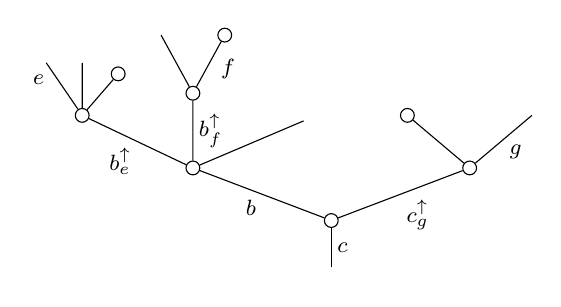
\begin{tikzpicture}[grow=up,auto,level distance=1.9em,
	every node/.style = {font=\footnotesize,inner sep=2pt},
	dummy/.style={circle,draw,inner sep=0pt,minimum size=1.75mm}]
		\node at (0,0) {}
			child{node [dummy] {}
				child[sibling distance = 10em]{node [dummy] {}
					child[sibling distance = 4.5em]{
					edge from parent node [swap] {$g$}}
					child[sibling distance = 4.5em]{node [dummy] {}}
				edge from parent node [swap] {$c_g^{\uparrow}$}}
				child[sibling distance = 10em]{node [dummy] {}
					child[sibling distance = 4em,level distance=1.7em]
					child[sibling distance = 1.5em,level distance=2.7em]{node [dummy] {}
						child[level distance=2.1em,sibling distance = 2.3em]{node [dummy] {}
						edge from parent node [near end,swap] {$f$}}		
						child[level distance=2.1em,sibling distance = 2.3em]{
						edge from parent node [near end] {}}
					edge from parent node [swap] {$b^{\uparrow}_{f}$}}
					child[sibling distance = 4em]{node [dummy] {}
						child[sibling distance =1.3em, level distance = 1.5 em]{node [dummy]  {}
						edge from parent node [swap] {}}
						child[sibling distance = 1.3em]{
						edge from parent node [very near end,swap] {}}
						child[sibling distance =1.3em]{
						edge from parent node [very near end] {$e$}}
					edge from parent node {$b^{\uparrow}_e$}}
				edge from parent node {$b$}}
			edge from parent node [swap] {$c$}};
	\end{tikzpicture}
\]
\end{example}

\begin{notation}
	Given a set $S$ of size $n$ we write
	$\textsf{Ord}(S) \simeq \mathsf{Iso}(S,\{1,\cdots,n\})$. We will usually abuse notation by regarding its objects as pairs $(S,\leq)$ where $\leq$ is a total order in $S$.
\end{notation}


\begin{proposition}\label{PLANARIZATIONCHAR PROP}
	Let $T \in \Omega$ be a tree. There is a bijection
	\begin{equation}\label{PLANAR EQ}
	\begin{tikzcd}[row sep = 0.5em]
		\{\text{planar structures }(T,\leq_p)\} \ar[r] &
		\prod_{(a^{\uparrow} \leq a) \in V(T)} \mathsf{Ord}(a^{\uparrow}) \\
		\leq_p \ar[mapsto]{r} & (\leq_p|_{a^{\uparrow}})
	\end{tikzcd}	
	\end{equation}
\end{proposition}


\begin{proof}
We will keep the setup of Proposition \ref{INPUTPREDECESSORPROP PROP} throughout: $e, f$ are $\leq_d$-incomparable edges and we write $b = e \vee f$. 

	We first show that (\ref{PLANAR EQ}) is injective, i.e. that the restrictions $\leq_p|_{a^{\uparrow}}$ determine if 
	$e <_p f$ holds or not.
If $b^{\uparrow}_e <_p b^{\uparrow}_f$, the relations
$e \leq_d b^{\uparrow}_e <_p b^{\uparrow}_f \geq_d f$
and Definition \ref{PLANARIZE DEF} imply it must be $e <_p f$.
Dually, if $b^{\uparrow}_f <_p b^{\uparrow}_e$ then 
$f <_p e$. Thus 
$b^{\uparrow}_e <_p b^{\uparrow}_f \Leftrightarrow e <_p f$ and hence (\ref{PLANAR EQ}) is indeed injective.

To check that (\ref{PLANAR EQ}) is surjective, it suffices (recall that $e,f$ are assumed $\leq_d$-incomparable) to check that
defining $e \leq_p f$ to hold iff $b^{\uparrow}_e < b^{\uparrow}_f$ holds in $b^{\uparrow}$ yields a planar structure.

Antisymmetry and the total order conditions are immediate, and it thus remains to check the transitivity and planar conditions.
Transitivity of $\leq_p$ in the case $e' \leq_d e <_p f$ and the planar condition, which is the case $e <_p f \geq_d f'$, follow from Proposition \ref{INPUTPREDECESSORPROP PROP}(c). Transitivity of $\leq_p$ in the case $e <_p f \leq_d f'$
follows since either $e \leq_d f'$ or else $e,f'$ are $\leq_d$-incomparable, in which case one can apply \ref{INPUTPREDECESSORPROP PROP}(c) with the roles of $f,f'$ reversed.

It remains to check transitivity in the hardest case, that of 
$e <_p f <_p g$ with $\leq_d$-incomparable $f,g$.
We write $c = e \vee f \vee g$.
By the ``therefore'' part of Proposition \ref{TERNARYJOIN PROP}, either
\begin{inparaenum}
	\item[(i)] $e \vee f <_d c$, in which case 
	Proposition \ref{TERNARYJOIN PROP}
	implies 
	$c^{\uparrow}_e = c^{\uparrow}_f$ and transitivity follows;
	\item[(ii)] $f \vee g <_d c$, which follows just as (i);
	\item[(iii)]  
$e \vee f = f \vee g =c$, in which case 
$c^{\uparrow}_e <
c^{\uparrow}_f <
c^{\uparrow}_g $ in $c^{\uparrow}$
so that $c^{\uparrow}_e \neq c^{\uparrow}_g$ and by Proposition \ref{TERNARYJOIN PROP} it is also 
$e \vee g = c$ and transitivity follows.
\end{inparaenum}
\end{proof}


\begin{remark}\label{FORESTPLAN REM}
	Definition \ref{PLANARIZE DEF} readily extends to forests $F \in \Phi$. The analogue of Proposition \ref{PLANARIZATIONCHAR PROP} then states that the data of a planar structure is 
equivalent to total orderings of the nodes of $F$ together with a total ordering of its set of roots.
Indeed, this follows by either adapting the proof above or by noting that planar structures on $F$ are clearly in bijection with planar structures on the join tree $F \star \eta$ 
(cf. \cite[Def. 7.44]{Pe16b}), which adds a single edge $\eta$ to $F$, serving as the (unique) root of $F \star \eta$.
\end{remark}


When discussing the substitution procedure in Section \ref{SUBS SEC} we will find it convenient to work with a model for the category $\Omega$ that possesses exactly one representative of each possible planar structure on each tree or, more precisely, such that the only isomorphisms preserving the planar structures are the identities. On the other hand, using such a model for $\Omega$ throughout would, among other issues, make the discussion of faces in Section \ref{OUTTALL SEC} rather awkward.
We now outline our conventions to address such issues.


Let $\Omega^p$, the category of \textit{planarized trees}, denote the category with objects pairs $T_{\leq_p}=(T,\leq_p)$ of trees together with a planar structure  and morphisms the \textit{underlying} maps of trees (so that the planar structures are ignored).
There is a full subcategory $\Omega^s \hookrightarrow \Omega^p$, whose objects we call \textit{standard models}, of those $T_{\leq_p}$ whose underlying set is one of the sets $\underline{n} = \{1,2,\cdots,n\}$ and for which $\leq_p$ coincides with the canonical order. 
\begin{example}\label{STANDMODEL EX}
	Some examples of standard models, i.e. objects of $\Omega^s$, follow (further, (\ref{PLANAREX EQ}) can also be interpreted as such an example).
\begin{equation}\label{PLANAROMEGAEX1 EQ}
	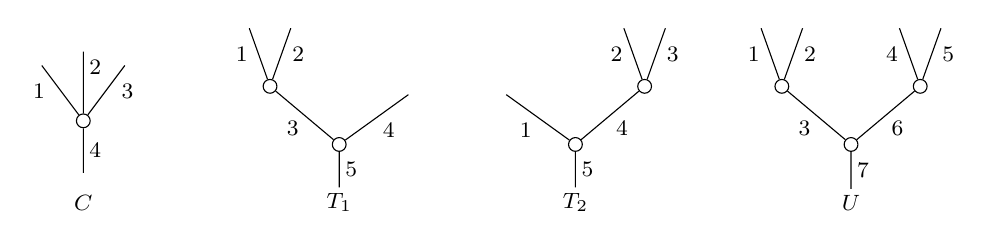
\begin{tikzpicture}[grow=up,auto,level distance=2.1em,
	every node/.style = {font=\footnotesize,inner sep=2pt},
	dummy/.style={circle,draw,inner sep=0pt,minimum size=1.75mm}]
		\node at (-0.25,0) {$C$};
		\node at (-0.25,0.3) {}
			child{node [dummy] {}
				child[sibling distance = 1.5em,level distance= 2em]{
				edge from parent node [swap, near end] {$3$}}
				child[sibling distance = 1.5em,level distance= 2.5em]{
				edge from parent node [swap, near end] {$2$}}
				child[sibling distance = 1.5em,level distance= 2em]{
				edge from parent node [near end] {$1$}}
			edge from parent node [swap] {$4$}};
		\node at (3,0) {$T_1$}
			child{node [dummy] {}
				child[sibling distance = 5em, level distance=1.8em]{
				edge from parent node [swap] {$4$}}
				child[sibling distance = 5em]{node [dummy] {}
					child[sibling distance = 1.5em]{
					edge from parent node [swap,near end] {$2$}}
					child[sibling distance = 1.5em]{
					edge from parent node [near end] {$1$}}
				edge from parent node {$3$}}
			edge from parent node [swap] {$5$}};
		\node at (6,0) {$T_2$}
			child{node [dummy] {}
				child[sibling distance = 5em]{node [dummy] {}
					child[sibling distance = 1.5em]{
					edge from parent node [swap,near end] {$3$}}
					child[sibling distance = 1.5em]{
					edge from parent node [near end] {$2$}}
				edge from parent node [swap] {$4$}}
				child[sibling distance = 5em, level distance=1.8em]{
				edge from parent node {$1$}}
			edge from parent node [swap] {$5$}};
		\node at  (9.5,0) {$U$}
			child{node [dummy] {}
				child[sibling distance = 5em]{node [dummy] {}
					child[sibling distance = 1.5em]{
					edge from parent node [swap,near end] {$5$}}
					child[sibling distance = 1.5em]{
					edge from parent node [near end] {$4$}}
				edge from parent node [swap] {$6$}}
				child[sibling distance = 5em]{node [dummy] {}
					child[sibling distance = 1.5em]{
					edge from parent node [swap,near end] {$2$}}
					child[sibling distance = 1.5em]{
					edge from parent node [near end] {$1$}}
				edge from parent node {$3$}}
			edge from parent node [swap] {$7$}};
	\end{tikzpicture}
\end{equation}
Here $T_1$ and $T_2$ are isomorphic to each other but not isomorphic to any other standard model in $\Omega^s$ while both $C$ and $U$ are the unique objects in their isomorphism classes. 
\end{example}


Given $T_{\leq_p} \in \Omega^p$ there is an obvious standard model $T_{\leq_p}^s \in \Omega^s$ given by replacing each edge by its order following $\leq_p$. Indeed, this defines a retraction 
$(\minus)^s \colon \Omega^p \to \Omega^s$
and a natural transformation 
$\sigma \colon id \Rightarrow (\minus)^s$
given by isomorphisms preserving the planar structure
(in fact, the pair $\left((\minus)^s, \sigma \right)$ is clearly unique).


\begin{convention}\label{PLANARCONV CON}
	From now on, we will write simply $\Omega$, $\Omega_G$ to denote the categories $\Omega^s$, $\Omega_G^s$ of standard models (where planar structures are defined in the underlying forest as in Remark \ref{FORESTPLAN REM}). 
Similarly $\mathsf{O}_G$ will denote the model $\mathsf{O}_G^s$ for the orbital category whose objects are the orbital $G$-sets whose underlying set is one of the sets $\underline{n} = \{1,2,\cdots,n\}$.

Therefore, whenever one of our constructions produces an object/diagram in $\Omega^p$, $\Omega^p_G$, $\mathsf{O}_G^p$ (of trees, $G$-trees, orbital $G$-sets with a planarization/total order) we will hence implicitly reinterpret it by using the standardization functor $(\minus)^s$.
\end{convention}

\begin{example}
To illustrate our convention, we consider the trees in Example \ref{STANDMODEL EX}. 

One has subfaces
$F_1 \subset F_2 \subset U$
where $F_1$ is the subtree with edge set $\{1,2,6,7\}$ and 
$F_2$ is the subtree with edge set $\{1,2,3,6,7\}$, both with inherited tree and planar structures. 
Applying $(\minus)^s$ to the inclusion diagram on the left below then yields a diagram as on the right.
\[
\begin{tikzcd}[row sep = 0.5em,column sep =1.3em]
	F_1 \ar[hookrightarrow]{rr} \ar[hookrightarrow]{rd} & & U & &&
	C \ar{rr} \ar{rd} & & U
\\
	& F_2 \ar[hookrightarrow]{ru} & & &&
	& T_1 \ar{ru}
\end{tikzcd}
\]
Similarly, let $\leq_{(12)}$ and $\leq_{(45)}$ denote alternate planar structures for $U$ exchanging the orders of the pairs $1,2$ and $4,5$, so that one has objects 
$U_{\leq_{(12)}}$, $U_{\leq_{(45)}}$ in $\Omega^p$. 
Applying $(\minus)^s$ to the diagram of underlying identities on the left yields the permutation diagram on the right.
\[
\begin{tikzcd}[row sep = 0.5em,column sep =1.3em]
	U \ar{rr}{id} \ar{rd}[swap]{id} & & U_{\leq_{(45)}} & & &
	U \ar{rr}{(45)} \ar{rd}[swap]{(12)} & & U
\\
	& U_{\leq_{(12)}} \ar{ru}[swap]{id} & & & &
	& U \ar{ru}[swap]{(12)(45)}
\end{tikzcd}
\]
\end{example}

\begin{example}
An additional reason to leave the use of $(\minus)^s$ implicit
is that when depicting $G$-trees it is preferable to choose edge labels that describe the action rather than the planarization (which is already implicit anyway).

For example, when $G = \mathbb{Z}_{/4}$, in both diagrams below the orbital representation on the left represents the isomorphism class consisting of the two trees $T_1,T_2 \in \Omega_G$ on the right.
\[
	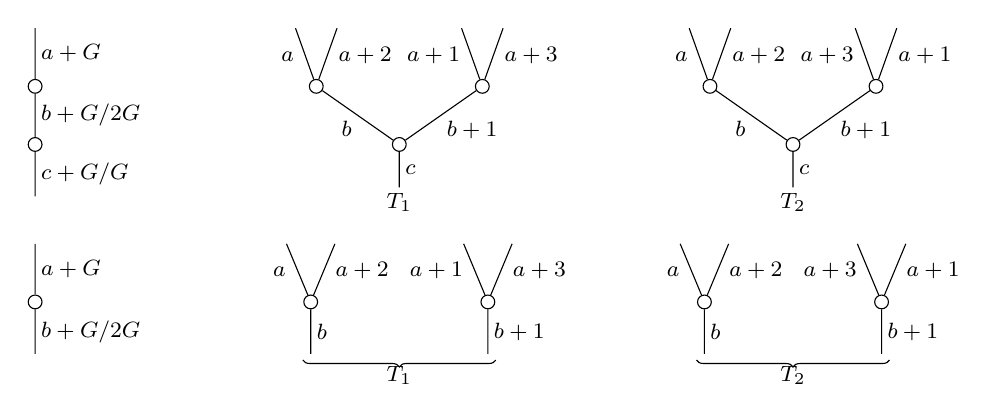
\begin{tikzpicture}[grow=up,auto,level distance=2.1em,
	every node/.style = {font=\footnotesize,inner sep=2pt},
	dummy/.style={circle,draw,inner sep=0pt,minimum size=1.75mm}]
		\node at (-1,0) {}
			child{node [dummy] {}
				child{node [dummy] {}
					child{
					edge from parent node [swap] {$a+G$}}
				edge from parent node [swap] {$b+G/2G$}}
			edge from parent node [swap] {$c + G/G$}};

		\node at  (3.625,0) {$T_1$}
			child{node [dummy] {}
				child[sibling distance = 6em]{node [dummy] {}
					child[sibling distance = 1.5em]{
					edge from parent node [swap,near end] {$a+3$}}
					child[sibling distance = 1.5em]{
					edge from parent node [near end] {$a+1$}}
				edge from parent node [swap] {$b+1$}}
				child[sibling distance = 6em]{node [dummy] {}
					child[sibling distance = 1.5em]{
					edge from parent node [swap,near end] {$a+2$}}
					child[sibling distance = 1.5em]{
					edge from parent node [near end] {$\phantom{0+}a$}}
				edge from parent node {$\phantom{1+}b$}}
			edge from parent node [swap] {$c$}};
		\node at  (8.625,0) {$T_2$}
			child{node [dummy] {}
				child[sibling distance = 6em]{node [dummy] {}
					child[sibling distance = 1.5em]{
					edge from parent node [swap,near end] {$a+1$}}
					child[sibling distance = 1.5em]{
					edge from parent node [near end] {$a+3$}}
				edge from parent node [swap] {$b+1$}}
				child[sibling distance = 6em]{node [dummy] {}
					child[sibling distance = 1.5em]{
					edge from parent node [swap,near end] {$a+2$}}
					child[sibling distance = 1.5em]{
					edge from parent node [near end] {$\phantom{0+}a$}}
				edge from parent node {$\phantom{1+}b$}}
			edge from parent node [swap] {$c$}};
		\node at (-1,-2) {}
			child{node [dummy] {}
				child[sibling distance=1.75em]{
				edge from parent node [swap]  {$a+G$}}
			edge from parent node [swap] {$b+G/2G$}};
		\node at (2.5,-2) {}
			child{node [dummy] {}
				child[sibling distance=1.75em]{
				edge from parent node [swap,near end] {$a+2$}}
				child[sibling distance=1.75em]{
				edge from parent node [near end]  {$\phantom{1+}a$}}
			edge from parent node [swap] {$b$}};
		\node at (4.75,-2) {}
			child{node [dummy] {}
				child[sibling distance=1.75em]{
				edge from parent node [swap,near end] {$a+3$}}
				child[sibling distance=1.75em]{
				edge from parent node [near end]  {$a+1$}}
			edge from parent node [swap] {$b+1$}};
		\draw[decorate,decoration={brace,amplitude=2.5pt}] (4.85,-2) -- (2.4,-2) node[midway]{$T_1$};
		\node at (7.5,-2) {}
			child{node [dummy] {}
				child[sibling distance=1.75em]{
				edge from parent node [swap,near end] {$a+2$}}
				child[sibling distance=1.75em]{
				edge from parent node [near end]  {$\phantom{1+}a$}}
			edge from parent node [swap] {$b$}};
		\node at (9.75,-2) {}
			child{node [dummy] {}
				child[sibling distance=1.75em]{
				edge from parent node [swap,near end] {$a+1$}}
				child[sibling distance=1.75em]{
				edge from parent node [near end]  {$a+3$}}
			edge from parent node [swap] {$b+1$}};
		\draw[decorate,decoration={brace,amplitude=2.5pt}] (9.85,-2) -- (7.4,-2) node[midway]{$T_2$};
	\end{tikzpicture}
\]
\end{example}


\begin{definition}
	A morphism $S \xrightarrow{\varphi} T$ in $\Omega$ that is compatible with the planar structures $\leq_p$ is called a 
	\textit{planar map}.
	
	More generally, a morphism $F \to G$ in the categories $\Phi$, $\Phi^G$, $\Omega^G$ of forests, $G$-forests, $G$-trees is called a \textit{planar map} if it is an independent map (cf. \cite[Def. 5.28]{Pe16b}) compatible with the planar structures $\leq_p$.
\end{definition}


\begin{remark}
	The need for the independence condition is justified by \cite[Lemma 5.33]{Pe16b} and its converse, since non independent maps do not reflect
 $\leq_d$ inequalities.
 
 We note that in the $\Omega_G$ case a map $\varphi$ is independent iff $\varphi$ does not factor through a non trivial quotient iff $\varphi$ is injective on each edge orbit.
\end{remark}


\begin{proposition}
\label{PLANARPULL EQ}
	Let $F \xrightarrow{\varphi} G$ be an independent map in $\Phi$ (or $\Omega$, $\Omega_G$, $\Phi_G$). Then there is a unique factorization 
	\[F \xrightarrow{\simeq} \bar{F} \to G\]
	such that $F \xrightarrow{\simeq} \bar{F}$ is an isomorphism and $\bar{F} \to G$ is planar.
\end{proposition}

\begin{proof}
We need to show that there is a unique planar structure 
$\leq_p^{\bar{F}}$ on the underlying forest of $F$ making the underlying map a planar map.
Simplicity of $G$ ensures that for any vertex $e^{\uparrow} \leq e$ of $F$ the edges in $\varphi(e^{\uparrow})$ are all distinct while independence of $\varphi$ likewise ensures that the edges in $\varphi(\underline{r}_F)$ are distinct.
The result now follows from (the forest version of) Proposition
\ref{PLANARIZATIONCHAR PROP}: one simply orders each set $e^{\uparrow}$ and $\underline{r}_F$ according to its image.

{\color{orange} not quite complete... maybe that $\leq_p$ is the closure of $\leq_d$ and the vertex relations under transitivity and the planar condition}
\end{proof}



\begin{remark}\label{PULLPLANAR REM}
	Proposition \ref{PLANARPULL EQ} says that planar structures  can be pulled back along independent maps. However, they can not always be pushed forward. As an example, in the notation of (\ref{PLANAROMEGAEX1 EQ}), consider the map $C \to T_1$ defined by $1 \mapsto 1$, $2 \mapsto 4$, $3 \mapsto 2$, $4 \mapsto 5$.
\end{remark}

\begin{remark}\label{UNIQCOR REM}
	Given any tree $T \in \Omega$ there is a unique corolla $\mathsf{lr}(T) \in \Sigma$ and planar tall map 
	$\mathsf{lr}(T) \to T$.
	Explicitly, the number of leaves of $\mathsf{lr}(T)$ matches that of $T$, together with the inherited order. 
\end{remark}


\subsection{Outer faces and tall maps}\label{OUTTALL SEC}



In preparation for our discussion of the substitution operation in Section \ref{SUBS SEC}, we now recall some basic notions and results concerning outer subtrees and tree grafting, as in \cite[Section 5]{Pe16b}.

\begin{definition}
	Let $T \in \Omega$ be a tree and 
	$e_1 \cdots e_n =\underline{e} \leq e$ a broad relation in $T$.
	
	We define the \textit{planar outer face $T_{\underline{e} \leq e}$}
	to be the subtree with underlying set those edges $f \in T$ such that
\begin{equation}\label{OUTERFACE EQ}
	f \leq_d e,\quad \forall_i e_i \nless_d f,
\end{equation}
generating broad relations the relations $f^{\uparrow} \leq f$ for $f$ satisfying (\ref{OUTERFACE EQ}) and $\forall_i f\neq e_i$,
and planar structure pulled back from $T$.
\end{definition}


\begin{remark}
If one forgoes the requirement that $T_{\underline{e} \leq e}$ be equipped with the pullback planar structure, the inclusion $T_{\underline{e} \leq e} \to T$ is usually called simply an \textit{outer face}.
\end{remark}

We now recap some basic results.

\begin{proposition}
Let $T \in \Omega$ be a tree.
\begin{itemize}
\item[(a)] $T_{\underline{e} \leq e}$ is a tree with root $e$
and edge tuple $\underline{e}$;
\item[(b)] there is a bijection
\[
	\{\text{planar outer faces of $T$} \} 
\leftrightarrow 
	\{\text{broad relations of $T$}\};
\]
\item[(c)] if $R \to S$ and $S \to T$ are outer face maps then so is $R \to T$;
\item[(d)] any pair of broad relations $\underline{g} \leq v$, $\underline{f}v \leq e$ induces a grafting pushout diagram
\begin{equation}\label{GRAPTPUSH EQ}
\begin{tikzcd}
	\eta \ar{r}{v} \ar{d}[swap]{v} & T_{\underline{g} \leq v} \ar{d}
\\
	T_{\underline{f}v \leq e} \ar{r} & T_{\underline{f}\underline{g} \leq v}
\end{tikzcd}
\end{equation}
%\item[(e)] a face map $S \to T$ is an outer face map iff whenever the composite relation $\underline{f} \underline{g} \leq e$ is in $S$ then so are the relations $\underline{g} \leq v$ and
%$\underline{f}v \leq e$.
\end{itemize}
\end{proposition}


\begin{proof}
We first show (a). That $T_{\underline{e} \leq e}$ is indeed a tree is the content of \cite[Prop. 5.20]{Pe16b}: more precisely, 
$T_{\underline{e} \leq e} = (T^{\leq e})_{\less \underline{e}}$
in the notation therein. That the root of $T_{\underline{e} \leq e}$ is $e$ is clear and that the root tuple is $\underline{e}$ follows from \cite[Remark 5.23]{Pe16b}.

 (b) follows from (a), which shows that $\underline{e} \leq e$ can be recovered from
$T_{\underline{e} \leq e}$.

 (c) follows from the definition of outer face together with \cite[Lemma 5.33]{Pe16b}, which states that the $\leq_d$ relations on $S,T$ coincide.
 
  Since by (c) both $T_{\underline{g} \leq v}$ and $T_{\underline{f}v \leq e}$ are outer faces of $T_{\underline{f} \underline{g} \leq v}$, 
(d) is a restatement of \cite[Prop. 5.15]{Pe16b}. 
%Since $\underline{e} \leq e$ is a broad relation in $T_{\underline{e} \leq e}$ (this follows from (a) together with \cite[Lemma 5.13]{Pe16b})
\end{proof}

\begin{definition}
	A map $S \xrightarrow{\varphi} T$ in $\Omega$ is called a \textit{tall map} if 
	\[\varphi(\underline{l}_S) = \underline{l}_T, 
		\qquad
	\varphi(r_S)= r_T,\]
where $l_{(\minus)}$ denotes the leaf tuple and $r_{(\minus)}$ the root.
\end{definition}


The following is a restatement of \cite[Cor. 5.24]{Pe16b}

\begin{proposition}\label{TALLOUTERDEC COR}
	Any map $S \xrightarrow{\varphi} T$ in $\Omega$ has a factorization, unique up to unique isomorphism,
	\[
		S \xrightarrow{\varphi^t} U \xrightarrow{\varphi^u} T
	\]
	as a tall map followed by an outer face (in fact, 
	$U= T_{\varphi(\underline{l}_S) \leq r_S}$).
\end{proposition}

We recall that a face $F \to T$ is called inner if is obtained by iteratively removing inner edges, i.e. edges other than the root or the leaves. In particular, it follows that a face is inner iff it is tall. The usual face-degeneracy decomposition thus combines with Corollary \ref{TALLOUTERDEC COR} to give the following.

\begin{corollary}
	Any map $S \xrightarrow{\varphi} T$ in $\Omega$ has a factorization, unique up to unique isomorphisms,
	\begin{equation}\label{TRIPLEFACT EQ}
		S \xrightarrow{\varphi^-} U \xrightarrow{\varphi^i} V \xrightarrow{\varphi^u} T
	\end{equation}
	as a degeneracy followed by an inner face followed by an outer face.
\end{corollary}
	
\begin{proof}
	The factorization (\ref{TRIPLEFACT EQ}) can be built by first performing the degeneracy-\-face decomposition and then performing the tall-outer decomposition on the face map.
\end{proof}


\subsection{Substitution}\label{SUBS SEC}


One of the key ideas needed to describe operads is that of substitution of tree nodes, a process that we will prefer to repackage in terms of maps of trees. We start by discussing an example, focusing on the related notion of 
 iterated graftings of trees (as described in (\ref{GRAPTPUSH EQ})).

\begin{example} The trees $U_1, U_2,\cdots, U_6$ on the left below can be grafted into the tree $U$ in the middle.
More precisely (among other possible grafting orders), one has
\begin{equation}\label{UFORMULA EQ}
U = \left(
		\left(
			\left(
				\left(
					\left(U_6 \amalg_a U_2 \right)
				\right) \amalg_a U_1
			\right) \amalg_b U_3
		\right) \amalg_d U_5
	\right) \amalg_c U_4
\end{equation}
\begin{equation}\label{SUBSDATUMTREES EQ}
	\begin{tikzpicture}[grow=up,auto,level distance=2.1em,
	every node/.style = {font=\footnotesize,inner sep=2pt},
	dummy/.style={circle,draw,inner sep=0pt,minimum size=1.25mm}]
\begin{scope}[xshift=-2em]
	\begin{scope}
	\tikzstyle{level 2}=[sibling distance=2.25em]%
	\tikzstyle{level 3}=[sibling distance=1.25em]%
		\node at (-0.25,3.2) {$U_1$}
			child{node [dummy] {}
				child
				child{node [dummy] {}
					child
					child
				}
			edge from parent node {$a$}};
	\end{scope}
		\node at (-0.25,1.5) {$U_2$}
			child{
		edge from parent node {$a$}};
		\node at (1.15,1.5) {$U_3$}
			child{node [dummy] {}
		edge from parent node {$b$}};
	\begin{scope}
	\tikzstyle{level 2}=[sibling distance=0.875em]%
		\node at (2.2,3.2) {$U_4$}
			child{node [dummy] {}
				child{node [dummy] {}}
				child{node [dummy] {}}
			edge from parent node {$c$}};
	\end{scope}
	\begin{scope}
		\tikzstyle{level 2}=[sibling distance=1.25em]%
		\node at (2.5,1.5) {$U_5$}
			child{node [dummy] {}
				child{node[dummy] {}}
				child{
				edge from parent node {$c$}}
			edge from parent node [swap] {$d$}};
	\end{scope}
	\begin{scope}
	\tikzstyle{level 2}=[sibling distance=3.5em]%
	\tikzstyle{level 3}=[sibling distance=2.25em]%
		\node at (1,-1) {$U_6$}
			child{node [dummy] {}
				child[sibling distance = 5em]{node [dummy] {}
					child[sibling distance = 3.5em]{edge from parent node [swap,near end] {$d$} }
					child[sibling distance = 3.5em]{edge from parent node [near end] {$b$} }
				}
				child[sibling distance = 7em]{ edge from parent node {$a$} }
			edge from parent node [swap] {$e$}};
	\end{scope}
\end{scope}
\begin{scope}[yshift=1em]
	\begin{scope}[level distance=2.3em]
	\tikzstyle{level 2}=[sibling distance=3.5em]%
	\tikzstyle{level 3}=[sibling distance=2.25em]%
	\tikzstyle{level 4}=[sibling distance=1.25em]%
	\tikzstyle{level 5}=[sibling distance=0.875em]%
		\node at (5.5,0) {$U$}
			child{node [dummy] {}
				child[sibling distance =5em]{node [dummy] {}
					child[sibling distance =3.5em]{node [dummy] {}
						child{node [dummy] {}
						}
						child{node [dummy] {}
							child{node [dummy] {}}
							child{node [dummy] {}}
						edge from parent node [near end] {$c$}}
					edge from parent node [swap, near end] {$d$}}
					child[sibling distance =3.5em]{node [dummy] {}
					edge from parent node [near end] {$b$}}
				}
				child[sibling distance =7em]{node [dummy] {}
					child
					child{node [dummy] {}
						child
						child
					}
				edge from parent node {$a$}}
			edge from parent node [swap] {$e$}};
	\end{scope}
	\begin{scope}[level distance=2.3em]
	\tikzstyle{level 2}=[sibling distance=2.3em]%
	\tikzstyle{level 4}=[sibling distance=1em]%
		\node at (10,0.3) {$T$}
			child{node [dummy] {}
				child{node [dummy] {}
					child{node [dummy] {}
					edge from parent node [swap] {$c$}}	
				edge from parent node [swap] {$d$}}
				child{node [dummy] {}
				edge from parent node [near end,swap] {$b$}}
				child{node [dummy] {}
					child{node [dummy] {}
						child
						child
						child
					edge from parent node {$a_1$}}
				edge from parent node {$a_2$}}
			edge from parent node [swap] {$e$}};
	\end{scope}
	\draw [->,dashed] (8.6,1.25) -- node {$\varphi$} (7.1,1.25);
\end{scope}
	\end{tikzpicture}
\end{equation}
We now consider the tree $T$, which is built by converting each $U_i$ into the corolla $\mathsf{lr}(U_i)$ (cf. Remark \ref{UNIQCOR REM}), and then performing the same grafting operations as in (\ref{UFORMULA EQ}). $T$ can then be regarded as encoding the combinatorics of the iterated grafting in (\ref{UFORMULA EQ}), with alternative ways to reorder operations in (\ref{UFORMULA EQ}) in bijection with ways to assemble $T$ out of its nodes.


One can now therefore think of the iterated grafting (\ref{UFORMULA EQ}) as being instead encoded by the tree $T$ together with the (unique) planar tall maps $\varphi_i$ below.
\begin{equation}\label{SUBSDATUMTREES2 EQ}
	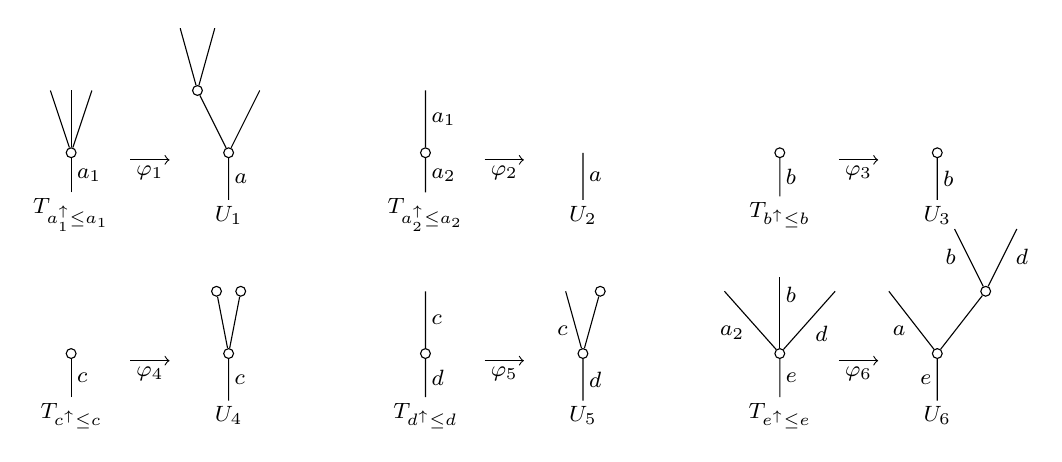
\begin{tikzpicture}[grow=up,auto,level distance=2.25em,
	every node/.style = {font=\footnotesize, inner sep=2pt},
	dummy/.style={circle,draw,inner sep=0pt,minimum size=1.25mm}]
	\begin{scope}
	\tikzstyle{level 2}=[sibling distance=0.75em]%
		\node at (0,0) {$T_{a_1^{\uparrow}\leq a_1}$}
			child{node [dummy] {}
				child
				child
				child
			edge from parent node [swap] {$a_1$}};
	\end{scope}	
	\begin{scope}
	\tikzstyle{level 2}=[sibling distance=2.25em]%
	\tikzstyle{level 3}=[sibling distance=1.25em]%
		\node at (2,0) {$U_1$}
			child{node [dummy] {}
				child
				child{node [dummy] {}
					child
					child
				}
			edge from parent node [swap] {$a$}};
	\end{scope}
		\draw [->] (0.75,0.7) -- node [swap]{$\varphi_1$} (1.25,0.7);
		\node at (4.5,0) {$T_{a_2^{\uparrow}\leq a_2}$}
			child{node [dummy] {}
				child{
				edge from parent node [swap] {$a_1$}}
			edge from parent node [swap] {$a_2$}};
		\node at (6.5,0) {$U_2$}
			child{
			edge from parent node [swap] {$a$}};
		\draw [->] (5.25,0.7) -- node [swap]{$\varphi_2$} (5.75,0.7);
		\node at (9,0) {$T_{b^{\uparrow}\leq b}$}
			child{node [dummy] {}
			edge from parent node [swap] {$b$}};
		\node at (11,0) {$U_3$}
			child{node [dummy] {}
			edge from parent node [swap] {$b$}};
		\draw [->] (9.75,0.7) -- node [swap]{$\varphi_3$} (10.25,0.7);
	\begin{scope}[yshift=-2.55cm]
		\node at (0,0) {$T_{c^{\uparrow}\leq c}$}
			child{node [dummy] {}
			edge from parent node [swap] {$c$}};
	\begin{scope}
	\tikzstyle{level 2}=[sibling distance=0.875em]%
		\node at (2,0) {$U_4$}
			child{node [dummy] {}
				child{node [dummy] {}}
				child{node [dummy] {}}
			edge from parent node  [swap]{$c$}};
	\end{scope}
	\draw [->] (0.75,0.7) -- node [swap]{$\varphi_4$} (1.25,0.7);
		\node at (4.5,0) {$T_{d^{\uparrow}\leq d}$}
			child{node [dummy] {}
				child{
				edge from parent node [swap] {$c$}}
			edge from parent node [swap] {$d$}};
	\begin{scope}
	\tikzstyle{level 2}=[sibling distance=1.25em]%
		\node at (6.5,0) {$U_5$}
			child{node [dummy] {}
				child{node[dummy] {}}
				child{
				edge from parent node {$c$}}
			edge from parent node [swap] {$d$}};
	\end{scope}
	\draw [->] (5.25,0.7) -- node [swap]{$\varphi_5$} (5.75,0.7);
	\begin{scope}
	\tikzstyle{level 2}=[sibling distance=2em]%
		\node at (9,0) {$T_{e^{\uparrow}\leq e}$}
			child{node [dummy] {}
				child{ edge from parent node [swap] {$d$} }
				child[level distance=2.75em]{ edge from parent node [near end,swap] {$b$} }
				child{ edge from parent node {$a_2$} }
			edge from parent node [swap] {$e$}};
	\end{scope}
	\begin{scope}
	\tikzstyle{level 2}=[sibling distance=3.5em]%
	\tikzstyle{level 3}=[sibling distance=2.25em]%
		\node at (11,0) {$U_6$}
			child{node [dummy] {}
				child{node [dummy] {}
					child{ edge from parent node [swap,near end] {$d$} }
					child{ edge from parent node [near end]{$b$} }
				}
				child{ edge from parent node {$a$} }
			edge from parent node {$e$}};
	\end{scope}
	\draw [->] (9.75,0.7) -- node [swap]{$\varphi_6$} (10.25,0.7);
	\end{scope}
	\end{tikzpicture}
\end{equation}
From this perspective, $U$ can now be thought as obtained from $T$ by substituting each of its nodes with the corresponding $U_i$. Moreover, the $\varphi_i$ assemble to a planar tall map 
$\varphi \colon T \to U$ (such that $a_i \mapsto a,b \mapsto b,\cdots,e \mapsto e$), which likewise encodes the same information.

Our perspective will then be that data for substitution of tree nodes such as in (\ref{SUBSDATUMTREES2 EQ}) can equivalently be 
repackaged using planar tall maps. 
\end{example}


\begin{definition}\label{SUBSTITUTIONDATUM}
	Let $T \in \Omega$ be a tree.
	
	A \textit{$T$-substitution datum} is a tuple 
	$\{U_{e^{\uparrow} \leq e}\}_{(e^{\uparrow} \leq e)\in V(T)}$ together with tall maps
	$T_{e^{\uparrow}\leq e} \to U_{e^{\uparrow}\leq e}$.
	
	Further, a map of planar $T$-substitution data 
	$\{U_{e^{\uparrow} \leq e}\} \to \{V_{e^{\uparrow} \leq e}\}$ is a tuple of tall maps $\{U_{e^{\uparrow} \leq e}\to V_{e^{\uparrow} \leq e}\}$ compatible with the chosen maps.
	
	Lastly, a substitution datum is called a $\textit{planar $T$-substitution datum}$ if the chosen maps are planar (so that 
	$\mathsf{lr}(U_{e^{\uparrow} \leq e}) = T_{e^{\uparrow} \leq e}$) and a morphism of planar data is called a planar morphism if it consists of a tuple of planar maps.
\end{definition}

\begin{definition}
	Let $T \in \Omega$. 
	
	The \textit{Segal core poset $\mathsf{Sc}(T)$} is the poset with objects the edge subtrees $\eta_e$ and vertex substrees $T_{e^{\uparrow} \leq e}$. The order relation is given by inclusion.
\end{definition}

\begin{remark}
Note that the only maps in $\mathsf{Sc}(T)$ are inclusions of the form $\eta_a \subset T_{e^{\uparrow}\leq e}$.
In particular, there are no pairs of composable non-identity relations in $\mathsf{Sc}(T)$. 
\end{remark}

Given a $T$-substitution datum $\{U_{\{e^{\uparrow}\leq e\}}\}$ we abuse notation by writing
\[U_{(\minus)} \colon \mathsf{Sc}(T) \to \Omega\]
for the functor $\eta_a \mapsto \eta$, $T_{e^{\uparrow} \leq e} \mapsto U_{e^{\uparrow} \leq e}$  
and sending the inclusions $\eta_a \subset T_{e^{\uparrow} \leq e}$
to the composites
\[
\eta \xrightarrow{a} T_{e^{\uparrow} \leq e}  \to 
%\simeq 
%\mathsf{lr}(U_{e^{\uparrow}\leq e}) \to 
U_{e^{\uparrow} \leq e}.\]


\begin{proposition}\label{SUBDATAUNDERPLAN PROP}
Let $T \in \Omega$ be a tree. There is an isomorphism of categories
\begin{equation}\label{SUBDATAUNDERPLAN EQ}
\begin{tikzcd}[row sep =0pt]
	\mathsf{Sub}_p(T) \ar[r,shift left=2pt] &
	\Omega_{T/}^{\mathsf{pt}} \ar[l,shift left=2pt]
\\
	\{U_{e^{\uparrow} \leq e}\} \ar[r,mapsto] & 
	\left(T \to \colim_{\mathsf{Sc}(T)} U_{(\minus)}\right)
\\
	\{U_{\varphi(e^{\uparrow}) \leq \varphi(e)}\} &
	(T \xrightarrow{\varphi} U) \ar[l,mapsto]
\end{tikzcd}
\end{equation}
where $\mathsf{Sub}_p(T)$ denotes the category of planar $T$-substitution data and $\Omega_{T/}^{\mathsf{pt}}$
the category of planar tall maps under $T$. 
\end{proposition}

\begin{proof}
We first claim that
\begin{inparaenum}
\item[(i)] the $\colim_{\mathsf{Sc}(T)} U_{(\minus)}$ indeed exists;
\item[(ii)] for the canonical datum $\{T_{e^{\uparrow}\leq e}\}$, it is $T = \colim_{\mathsf{Sc}(T)} T_{(\minus)}$;
\item[(iii)] the induced map
$T \to \colim_{\mathsf{Sc}(T)} U_{(\minus)}$ is planar tall.
\end{inparaenum}
 
The argument is by induction on the number of vertices of $T$, with the base cases of $T$ with $0$ or $1$ vertices being immediate, since then $T$ is the terminal object of $\mathsf{Sc}(T)$.
Otherwise, one can choose a non trivial grafting decomposition so as to write $T = R \amalg_e S$, resulting 
in identifications 
$\mathsf{Sc}(R) \subset \mathsf{Sc}(T)$, 
$\mathsf{Sc}(S) \subset \mathsf{Sc}(T)$
so that 
$\mathsf{Sc}(R) \cup \mathsf{Sc}(S) = \mathsf{Sc}(T)$
and 
$\mathsf{Sc}(R) \cap \mathsf{Sc}(S) = \{\eta_e \}$.
The existence of $\colim_{\mathsf{Sc}(T)}U_{(\minus)}$
is thus equivalent to the existence of the pushout below.
\begin{equation}\label{ASSEMBLYGRAFT EQ}
\begin{tikzcd}
	\eta \ar{r} \ar{d} & \colim_{\mathsf{Sc}(R)}U_{(\minus)} \ar[dashed,d]
\\
	\colim_{\mathsf{Sc}(S)}U_{(\minus)} \ar[dashed,r] &
	\colim_{\mathsf{Sc}(T)}U_{(\minus)}
\end{tikzcd}
\end{equation}
By induction, the top right and bottom left colimits exist for any $U_{(\minus)}$, 
equal $R$ and $S$ in the case $U_{(\minus)} = T_{(\minus)}$,
and the maps 
$R \to \colim_{\mathsf{Sc}(R)}U_{(\minus)}$,
$S \to \colim_{\mathsf{Sc}(S)}U_{(\minus)}$
are planar tall.
But is now follows that (\ref{ASSEMBLYGRAFT EQ}) is a grafting pushout diagram, so that the pushout indeed exists. The conditions that
$T = \colim_{\mathsf{Sc}(T)}T_{(\minus)}$
and 
$T \to \colim_{\mathsf{Sc}(T)}U_{(\minus)}$
is planar tall follow.

The fact that the two functors in (\ref{SUBDATAUNDERPLAN EQ})
are inverse to each other is clear by the same inductive argument.
\end{proof}


\begin{corollary}\label{SUBDATAUNDERPLAN COR}
Let $T \in \Omega$ be a tree. There is an isomorphism of categories
\begin{equation}\label{SUBDATAUNDERNONPL EQ}
\begin{tikzcd}[row sep =0pt]
	\mathsf{Sub}(T) \ar[r,shift left=2pt] &
	\Omega_{T/}^{\mathsf{t}} \ar[l,shift left=2pt]
\end{tikzcd}
\end{equation}
where $\mathsf{Sub}(T)$ denotes the category of $T$-substitution data and $\Omega_{T/}^{\mathsf{t}}$
the category of tall maps under $T$.
\end{corollary}


\begin{proof}
	This is a consequence of Proposition \ref{PLANARPULL EQ} together with the previous result, with the functor 
	$\mathsf{Sub}(T) \to \Omega_{T/}^{\mathsf{t}}$ given by the same formula.
	Indeed, Proposition \ref{PLANARIZATIONCHAR PROP} can be restated as saying that isomorphisms $T \to T'$ are in bijection with substitution data consisting of isomorphisms, and thus  bijectiveness reduces to that in the previous result.
\end{proof}


\begin{remark}\label{VERTEXDECOMP REM}
	It follows from the previous proof that, writing 
	$U = \colim_{\mathsf{Sc}(T)}U_{(\minus)}$,
	one has 
\begin{equation}\label{VERTEXDECOMP EQ}
	V(U) = \coprod_{(e^{\uparrow} \leq e) \in V(T)}
	V(U_{e^{\uparrow} \leq e}).
\end{equation}
Alternatively, (\ref{VERTEXDECOMP EQ}) can be regarded as a map 
$f^{\**} \colon V(U) \to V(T)$ induced by the planar tall map 
$f \colon T \to U$.
Explicitly, $f^{\**}(U_{u^{\uparrow} \leq u})$ 
is the unique $T_{t^{\uparrow}\leq t}$ such that
$U_{u^{\uparrow} \leq u} \subset U_{t^{\uparrow} \leq t}$. We note that $f^{\**}$ is indeed contravariant in the tall planar map $f$.
\end{remark}


The following is a converse of sorts to
 Proposition \ref{SUBDATAUNDERPLAN PROP}.

\begin{proposition}\label{BUILDABLE PROP}
	Let $U \in \Omega$ be a tree. Then:
\begin{itemize}
	\item[(i)] given non stick outer subtrees $U_i$ such that 
	$V(U) = \coprod_i V(U_i)$ there is a unique tree $T$ and planar tall map $T \to U$ such that $\{U_i\} = \{U_{e^{\uparrow}\leq e}\}$;
	\item[(ii)] given multiplicities $m_e \geq 1$ for each edge $e \in U$, there is a unique planar degeneracy $\rho \colon T \to U$ such that $\rho^{-1}(e)$ has $m_e$ elements;
	\item[(iii)] planar tall maps $T \to U$ are in bijection with collections $\{U_i\}$ of outer subtrees such that $V(U) = \coprod_i V(U_i)$ and $U_j$ is not an inner edge of any $U_i$ whenever $U_j \simeq \eta$ is a stick.
\end{itemize}
\end{proposition}


\begin{proof}
	We first show (i) by induction on the number of subtrees $U_i$. The base case $\{U_i\}=\{U\}$ is immediate, setting 
	$T= \mathsf{lr}(U)$. Otherwise, letting $e$ be edge that is both an inner edge of $U$ and a root of some $U_i$, and one can form a pushout diagram
\begin{equation} \label{DECOMPPROOF EQ}
\begin{tikzcd}
	\eta \ar{r}{e} \ar{d}[swap]{e} & V \ar{d}
\\
	W \ar{r} & U
\end{tikzcd}
\end{equation}
inducing a nontrivial partition 
$\{U_i\} = \{U_i|U_i \hookrightarrow V\} 
\amalg \{U_i|U_i \hookrightarrow W\}$. Existence of $T \to U$ now follows from the induction hypothesis. For uniqueness, the condition that no $U_i$ is a stick guarantees that $T$ possesses a single inner edge mapping to $e$, and thus admits a compatible decomposition as in (\ref{DECOMPPROOF EQ}), and thus uniqueness too follows by the induction hypothesis.

For (ii), we argue existence by nested induction on the number of vertices $|V(U)|$ and the sum of the multiplicities $m_e$. The base case $|V(U)|=0$, i.e., $U = \eta$ is immediate. Otherwise, writing $m_e = m'_e +1$, one can form a decomposition (\ref{DECOMPPROOF EQ}) where either $|V(V)|,|V(W)|<|V(U)|$ or one of $V,W$ is $\eta$, so that $T \to U$ can be built via the induction hypothesis. For uniqueness, note first that 
by \cite[Lemma 5.33]{Pe16b} each pre-image $\rho^{-1}(e)$ is linearly ordered and by the ``further'' claim in 
\cite[Cor. 5.39]{Pe16b} the remaining broad relations are precisely the pre-image of the non-identity relations in $U$, showing that the tree $T$ is uniquely determined.

(iii) follows by combining (i) and (ii). Indeed, any planar tall map $T \to U$ has a unique decomposition 
$T \twoheadrightarrow \bar{T} \hookrightarrow U$
as a planar degeneracy followed by a planar inner face, and each  of these maps is classified by the data in (b) and (a).
\end{proof}


\begin{lemma}\label{OUTERFACEUNION LEM}
	Suppose $T_1,T_2 \hookrightarrow T$ are two outer faces with at least one common edge $e$. Then there exists an unique outer face $T_1 \cup T_2$ such that 
	$V(T_1 \cup T_2) = V(T_1) \cup V(T_2)$.
\end{lemma}

\begin{proof}
	If either of $T_1,T_2$ is the root or a leaf the result is obvious. Otherwise, one can necessarily choose $e$ to be an inner edge of $T$, in which case all of $T_1,T_2,T$ admit compatible decompositions (\ref{DECOMPPROOF EQ}) and the result follows by induction on $|V(T)|$.
\end{proof}



\section{The genuine equivariant operad monad}

We now turn to the task of building the monad encoding genuine equivariant operads.



\subsection{Wreath product over finite sets}

In what follows we will let $\Fin$ denote the usual skeleton of the category of finite sets and all set maps. Explicitly, its objects are the finite sets $\{1,2,\cdots,n\}$ for $n\geq 0$.
However, much as in the discussion in 
Convention \ref{PLANARCONV CON} we will often find it more convenient to regard the elements of $\Fin$ as equivalence classes of finite sets equipped with total orders.
 

\begin{definition}
	For a category $\C$, we let $\Fin \wr \C$ denote the opposite of the Grothendieck construction for the functor
\[
\begin{tikzcd}[row sep=0pt]
	\Fin^{op} \ar{r} & \mathsf{Cat}
\\
	I \ar[r,mapsto] & \C^I
\end{tikzcd}	
 \]
Explicitly, the objects of $\Fin \wr \C$ are tuples $(c_i)_{i \in I}$ and a map 
$(c_i)_{i \in I} \to (d_j)_{j \in J}$ consists of a pair 
\[(\phi \colon I \to J, (f_i\colon c_i \to d_{\phi(i)})_{i\in I}),\]
 henceforth abbreviated as $(\phi,(f_i))$.
\end{definition}
 
 The following is immediate.

\begin{proposition}
	Suppose $\C$ has all finite coproducts. One then has a functor as on the left below.
Dually, if $\C$ has all finite products, one has a functor as on the right below.
\[
\begin{tikzcd}[row sep=0pt]
	\Fin \wr \C \ar{r}{\coprod} & \C & &
	(\Fin \wr \C^{op})^{op} \ar{r}{\prod} & \C
\\
	(c_i)_{i \in I} \ar[mapsto]{r} & \coprod_{i \in I}{c_i} & &
	(c_i)_{i \in I} \ar[mapsto]{r} & \prod_{i \in I}{c_i}
\end{tikzcd}
\]
\end{proposition}



\begin{lemma}\label{FINWREATPRODLIM LEM}
Suppose that $\mathcal{E}$ is a bicomplete category such that 
coproducts commute with limits in each variable. If the leftmost diagram
\begin{equation}\label{WRRAN EQ}
	\begin{tikzcd}
	\mathcal{C} \ar{r}[swap,name=F]{}{F} \ar{d}[swap]{k} &
	\mathcal{E} & 
	& 
	\Fin \wr \mathcal{C} \ar{r}[swap,name=FF]{}{\Fin \wr F} \ar{d}[swap]{\Fin \wr k}&
	\Fin \wr \mathcal{E} \ar{r}{\amalg} &
	\mathcal{E}
		\\
	|[alias=D]|\mathcal{D} \ar{ru}[swap]{G} &
	& & 
	|[alias=FD]|\Fin \wr \mathcal{D} \ar{ru}[swap]{\Fin \wr G}
	\ar[bend right=13]{rru}[swap]{\amalg \circ \Fin \wr G}
	\arrow[Rightarrow, from=D, to=F,shorten <=0.10cm,"\eta"]
	\arrow[Rightarrow, from=FD, to=FF,shorten <=0.10cm,"\Fin \wr \eta"]
	\end{tikzcd}
\end{equation}
is a right Kan extension diagram then so is the composite of the rightmost diagram. 

Dually, if in $\mathcal{E}$ products commute with colimits in each variable, and the leftmost diagram
\begin{equation}\label{WRLAN EQ}
	\begin{tikzcd}[column sep = 4.5em]
	\mathcal{C}^{op} \ar{r}[swap,name=F]{}{F} \ar{d}[swap]{k} & 
	\mathcal{E} & 
	(\Fin \wr \mathcal{C})^{op} \ar{d}[swap]{(\Fin \wr k^{op})^{op}} 
	\ar{r}[swap,name=FF]{}{(\Fin \wr F^{op})^{op}} & 
	(\Fin \wr \mathcal{E}^{op})^{op} \ar{r}{\Pi} &
	\mathcal{E}
	\\
	|[alias=D]|\mathcal{D}^{op} \ar{ru}[swap]{G} &
	& 
	|[alias=FD]|(\Fin \wr \mathcal{D})^{op} 
	\ar{ru}[swap]{(\Fin \wr G^{op})^{op}}
	\ar[bend right=13]{rru}[swap]{\Pi \circ (\Fin \wr G^{op})^{op}}
	&
	\arrow[Leftarrow, from=D, to=F,shorten <=0.10cm,"\epsilon"]
	\arrow[Leftarrow, from=FD, to=FF,shorten <=0.10cm]
	\end{tikzcd}
\end{equation}
is a left Kan extension diagram then so is the composite of the rightmost diagram. 
\end{lemma}


\begin{proof}
	Unpacking definitions using the pointwise formula for Kan extensions (\cite[X.3.1]{McL}), the claim concerning (\ref{WRRAN EQ}) amounts to showing that for each $(d_i) \in \Fin \wr \mathcal{D}$ one has natural isomorphisms
	\begin{equation}\label{POINTKAN EQ}
	\underset{((d_i) \to (kc_j))\in
	\left( (d_i) \downarrow \Fin \wr \C \right) }{\lim} {\left(\coprod_j{F(c_j)}\right)}
		\simeq	
	\coprod_i \underset{(d_i  \to kc_i) \in d_i \downarrow \C}{\lim}
	\left(F(c_i)\right).
	\end{equation}
Noting that the canonical factorizations of each $(\varphi,(f_i))\colon (d_i)_{i \in I} \to (k c_j)_{j \in J}$ as
\[(d_i)_{i\in I} \to (c_{\phi(i)})_{i \in I} \to (k c_j)_{j \in J}\]
exhibit $\prod_{i}{(d_i\downarrow \mathcal{C})}$ as a coreflexive subcategory of $(d_i)\downarrow \Fin \wr \mathcal{C}$, we see that it is an initial subcategory. Therefore
	\[
	\underset{((d_i) \to (kc_j))\in
	\left( (d_i)\downarrow \Fin \wr \C \right) }{\lim} {\left(\coprod_j{F(c_j)}\right)}
		\simeq	
	\underset{((d_i) \to (kc_i))\in
	\prod_{i} \left( {d_i \downarrow \mathcal{D}} \right)}{\lim}
	\left(\coprod_i{F(c_i)}\right)
	\]
and hence (\ref{POINTKAN EQ}) now follows from the assumption that coproducts commute with limits in each variable.
\end{proof}

\begin{notation}
Using the coproduct functor $\Fin^{\wr 2} = \Fin^{\wr \{{0,1\}}} =\Fin \wr \Fin \xrightarrow{\amalg} \Fin$ (where $\coprod_{i\in I} J_i$ is ordered lexicographically) and the simpleton $\{1\} \in \Fin$
one can regard the collection of categories 
$\Fin^{\wr \{0,\cdots,n\}} \wr \C = \Fin^{\wr \underline{n}} \wr \C$
 as a coaugmented cosimplicial object in $\mathsf{Cat}$.
As such, we will denote by
\[
	\delta^i\colon \Fin^{\wr \underline{n-1}} \wr \C \to \Fin^{\wr \underline{n}} \wr \C, \qquad 0 \leq i \leq n
\]
the cofaces obtained by inserting simpletons $\{1\} \in \Fin$ and by 
\[
	\sigma^i \colon \Fin^{\wr \underline{n+1}} \wr \C \to \Fin^{\wr \underline{n}} \wr \C, \qquad 0 \leq i \leq n
\]
the codegeneracies obtained by applying the coproduct 
$\Fin^{\wr 2} \xrightarrow{\amalg} \Fin$ to adjacent 
$\Fin$ coordinates.
\end{notation}



\subsection{Equivariant leaf-root and vertex functors}

\begin{definition}
	A morphism $T \xrightarrow{\varphi} S$ in $\Omega_G$ is called a \textit{quotient} if the underlying morphism of forests
	\[\coprod_{[g]\in G/H} {T_{[g]} } 
	\to
	\coprod_{[h]\in G/K} {S_{[h]} } 
	\]
maps each tree component (or, equivalently, some tree component) isomorphically onto its image component.

We denote the subcategory of $G$-trees and quotients by $\Omega_G^q$.
\end{definition}


\begin{definition}
	The \textit{$G$-symmetric category}, which we will also call the \textit{category of $G$-corollas}, is the full subcategory 
	$\Sigma_G \subset \Omega_G^{q}$ of those $G$-trees that are corollas, i.e. $G$-trees such that each edge is either a root or a leaf (but not both).
\end{definition}


\begin{definition}
	The \textit{leaf-root functor} is the functor $\Omega_G^q \xrightarrow{\mathsf{lr}} \Sigma_G$ defined by 
	\[
	 \mathsf{lr}(T)=\{\text{leaves of }T\}\amalg \{\text{roots of }T\}
	\]
	with a broad relation $l_1 \cdots l_n \leq r$ holding in 
	$\mathsf{lr}(T)$ iff its image holds in $T$ and similarly for the planar structure $\leq_p$.
\end{definition}

\begin{remark}\label{LEAFROOTEXAMP REM}
	Generalizing Remark \ref{UNIQCOR REM},
	$\mathsf{lr}(T)$ can alternatively be characterized as being the \textit{unique} $G$-corolla which admits an also unique (tree-wise) tall planar map $\mathsf{lr}(T) \to T$. Moreover, $\mathsf{lr}(T)$ can usually be regarded as the ``smallest inner face'' of $T$, obtained by removing all the inner edges, although this characterization fails when 
	$T=G\cdot_H \eta$ is a stick $G$-tree. Some examples with $G=\mathbb{Z}_{/4}$ follow.
\[
	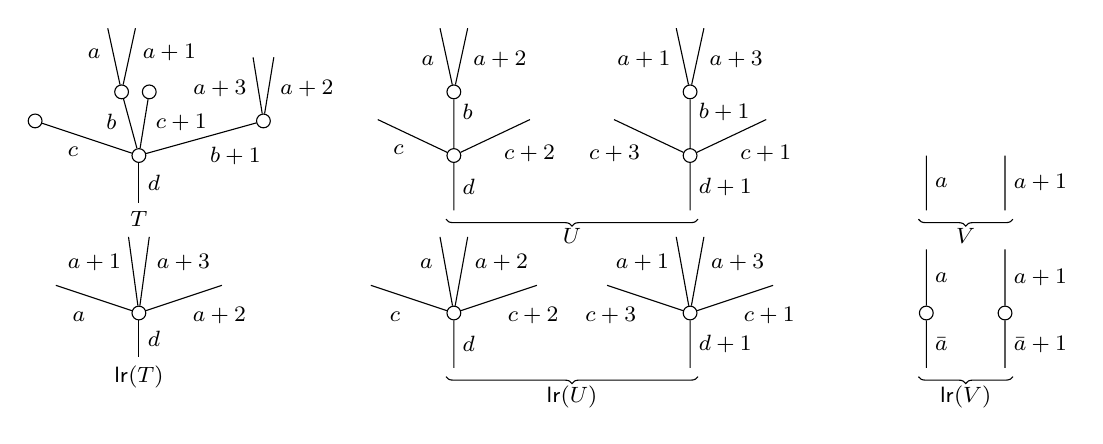
\begin{tikzpicture}[grow=up,auto,level distance=2.3em,
	every node/.style = {font=\footnotesize,inner sep=3pt},
	dummy/.style={circle,draw,inner sep=0pt,minimum size=1.75mm}]
		\node at (0,0) {$T$}
			child{node [dummy] {}
				child[level distance=1.25em,sibling distance = 3em]{node [dummy] {}
					child[level distance=2.3em,sibling distance =0.75em]{
					edge from parent node [swap,near end] {$a+2$}}
					child[level distance=2.3em,sibling distance =0.75em]{
					edge from parent node [near end] {$a+3$}}
				edge from parent node [swap] {$b+1$}}
				child[sibling distance = 0.75em]{node [dummy] {}
				edge from parent node [swap, very near end] {$c+1$}}
				child[sibling distance = 1.25em]{node [dummy] {}
					child[sibling distance = 1em]{
					edge from parent node [swap,very near end] {$a+1$}}
					child[sibling distance = 1em]{
					edge from parent node [very near end] {$\phantom{1+}a$}}
				edge from parent node [very near end] {$b$}}
				child[level distance=1.25em,sibling distance = 2.5em]{node [dummy] {}
				edge from parent node {$c$}}
			edge from parent node [swap] {$d$}};
		\node at (0,-2) {$\mathsf{lr}(T)$}
			child{node [dummy] {}
				child[sibling distance=2em, level distance=1em]{
				edge from parent node [swap] {$a+2$}}
				child[sibling distance=0.75em,level distance=2.75em]{
				edge from parent node [very near end,swap] {$a+3$}}
				child[sibling distance=0.75em,level distance=2.75em]{
				edge from parent node [very near end] {$a+1$}}
				child[sibling distance=2em, level distance=1em]{
				edge from parent node {$\phantom{1+}a$}}
			edge from parent node [swap] {$d$}};
		\node at (4,0) {}
			child{node [dummy] {}
				child[level distance=1.3em,sibling distance=2.75em]{
				edge from parent node [swap] {$c+2$}}
				child{node [dummy] {}
					child[sibling distance=1em]{
					edge from parent node [near end,swap] {$a+2$}}
					child[sibling distance=1em]{
					edge from parent node [near end] {$\phantom{1}a$}}
				edge from parent node [swap, near end] {$b$}}
				child[level distance=1.3em,sibling distance=2.75em]{
				edge from parent node {$c$}}
			edge from parent node [swap] {$d$}};
		\node at (7,0) {}
			child{node [dummy] {}
				child[level distance=1.3em,sibling distance=2.75em]{
				edge from parent node [swap] {$c+1$}}
				child{node [dummy] {}
					child[sibling distance=1em]{
					edge from parent node [near end,swap] {$a+3$}}
					child[sibling distance=1em]{
					edge from parent node [near end] {$a+1$}}
				edge from parent node [swap, near end] {$b+1$}}
				child[level distance=1.3em,sibling distance=2.75em]{
				edge from parent node {$c+3$}}
			edge from parent node [swap] {$d+1$}};
			\draw[decorate,decoration={brace,amplitude=2.5pt}] (7.1,0) -- (3.9,0) node[midway]{$U$};
		\node at (4,-2) {}
			child{node [dummy] {}
				child[sibling distance=2em, level distance=1em]{
				edge from parent node [swap] {$c+2$}}
				child[sibling distance=1em,level distance=2.75em]{
				edge from parent node [very near end,swap] {$a+2$}}
				child[sibling distance=1em,level distance=2.75em]{
				edge from parent node [very near end] {$\phantom{1+}a$}}
				child[sibling distance=2em, level distance=1em]{
				edge from parent node {$\phantom{1+}c$}}
			edge from parent node [swap] {$d$}};
		\node at (7,-2) {}
			child{node [dummy] {}
				child[sibling distance=2em, level distance=1em]{
				edge from parent node [swap] {$c+1$}}
				child[sibling distance=1em,level distance=2.75em]{
				edge from parent node [very near end,swap] {$a+3$}}
				child[sibling distance=1em,level distance=2.75em]{
				edge from parent node [very near end] {$a+1$}}
				child[sibling distance=2em, level distance=1em]{
				edge from parent node {$\phantom{1+}c+3$}}
			edge from parent node [swap] {$d+1$}};
			\draw[decorate,decoration={brace,amplitude=2.5pt}] (7.1,-2) -- (3.9,-2) node[midway]{$\mathsf{lr}(U)$};
			\node at (10,0) {}
				child{
				edge from parent node [swap] {$a$}};
			\node at (11,0) {}
				child{
				edge from parent node [swap] {$a+1$}};
			\draw[decorate,decoration={brace,amplitude=2.5pt}] (11.1,0) -- (9.9,0) node[midway]{$V$};
			\node at (10,-2) {}
				child{node[dummy]{}
					child{
					edge from parent node [swap] {$a$}}
				edge from parent node [swap] {$\bar{a}$}};
			\node at (11,-2) {}
				child{node[dummy]{}
					child{
					edge from parent node [swap] {$a+1$}}
				edge from parent node [swap] {$\bar{a}+1$}};
			\draw[decorate,decoration={brace,amplitude=2.5pt}] (11.1,-2) -- (9.9,-2) node[midway]{$\mathsf{lr}(V)$};
	\end{tikzpicture}
\]	
\end{remark}


\begin{remark}
	One consequence of the fact that planarizations can not be pushed forward along tree maps (cf. Remark \ref{PULLPLANAR REM})
is that $\mathsf{lr} \colon \Omega_G^q \to \Sigma_G$ is not a categorical fibration.
{\color{red} maybe add to this}.
\end{remark}


\begin{definition}\label{VG DEF}
	Given $T \in \Omega_G$ we define the set $V_G(T)$ of 
	\textit{$G$-vertices} of $T$ to be the orbit set $V(T)/G$, i.e. the quotient of the vertex set $V(T)$ by its $G$-action.
	
Furthermore, we will regard $V_G(T)$ as an object in $\Fin$ by equipping it with its lexicographic order: i.e. vertex equivalence classes $[e^{\uparrow} \leq e]$ are ordered according to the planar order $\leq_p$ of the smallest representative $ge$, $g \in G$.
\end{definition}



\begin{remark}\label{VERTEXDECOMPG REM}
	Following Remark \ref{VERTEXDECOMP REM},
	a planar tall map $f \colon T \to U$ of $G$-trees
	induces a $G$-equivariant map
	$f^{\**} \colon V(U) \to V(T)$
	and thus also a map of orbits
	$f^{\**} \colon V_G(U) \to V_G(T)$.
We note, however, that $f^{\**}$ is not in general compatible with the order on $V_G$, as is indeed the case even in the non-equivariant case.

A minimal example follows.
		\[
		\begin{tikzpicture}[grow=up,auto,level distance=2.4em,
		every node/.style = {font=\footnotesize},
		dummy/.style={circle,draw,inner sep=0pt,minimum size=1.75mm}]
		\node at (0,0) {$T$}
			child{node [dummy] {}
				child[sibling distance = 3.5em]{node [dummy] {}
					child
				edge from parent node[swap] {$c$}}
				child[level distance=2.9em]{
				edge from parent node [swap] {$b$}}
				child[sibling distance = 3.5em]{node [dummy] {}
					child
				edge from parent node {$a$}}		
			edge from parent node [swap] {$d$}};
		\node at (6,0) {$U$}
			child{node [dummy] {}
				child[sibling distance = 5em]{node [dummy] {}
					child
				edge from parent node [swap] {$c$}}
				child[sibling distance = 5em]{node [dummy] {}
					child[sibling distance = 3.5em]{
					edge from parent node [swap,near end] {$b$}}
					child[sibling distance = 3.5em]{node [dummy] {}
						child
					edge from parent node [near end]{$a$}}
				edge from parent node {$e$}}
			edge from parent node [swap] {$d$}};
		\draw[->] (2.6,1) -- node [above] {$f$} (3.6,1) ;
		\end{tikzpicture}
		\]
In $V(T)$ the vertices are ordered as $a<c<d$ while in $V(U)$ they are ordered as $a<e<c<d$ but the map 
$f^{\**} \colon V(U) \to V(T)$ is given by 
$a \mapsto a, c \mapsto c, d \mapsto d, e \mapsto d$.
\end{remark}


Note that each element of $V_G(T)$ corresponds to an unique edge orbit $Ge$ for $e$ not a leaf. As such, we will represent the corresponding $G$-vertex by $v_{Ge}=(Ge)^{\uparrow} \leq Ge$ (which we interpret as the concatenation of the relations $f^{\uparrow} \leq f$ for $f \in G e$) and write
\[T_{v_{Ge}}=T_{(Ge)^{\uparrow} \leq Ge} = \coprod_{f\in Ge} T_{f^{\uparrow}\leq f}.\]
We note that $T_{v_{Ge}}$ is always a $G$-corolla. Indeed, noting that a quotient map $\varphi \colon T \to S$ induces quotient maps 
$T_{v_{ge}} \to S_{v_{G\varphi(e)}}$ one obtains a functor
	\begin{equation}\label{VFUNCTOR EQ}
		\begin{tikzcd}[row sep=tiny]
		\Omega_G^q \ar{r}{V_G} & \Fin \wr \Sigma_G \\
		T \ar[mapsto]{r} & (T_{v_{Ge}})_{v_{Ge} \in V_G(T)}.
		\end{tikzcd}	
	\end{equation}

\begin{remark}
	The need to introduce the $\Fin \wr \C$ categories comes from the fact that general quotient maps do not preserve the number of $G$-vertices. For a simple example, let $G=\mathbb{Z}_{/4}$ and consider the quotient map
		\[
		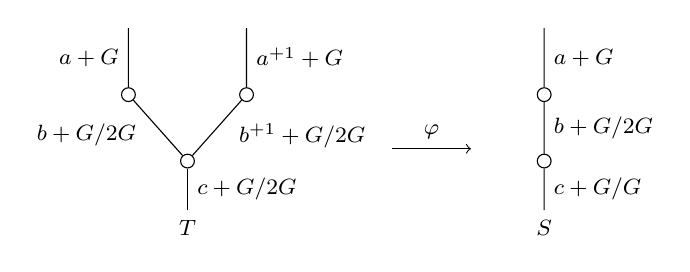
\begin{tikzpicture}[grow=up,auto,level distance=2.4em,every node/.style = {font=\footnotesize},dummy/.style={circle,draw,inner sep=0pt,minimum size=1.75mm}]
		\node at (0,0) {$T$}
			child{node [dummy] {}
				child{node [dummy] {}
					child{
					edge from parent node [swap] {$a^{+1} + G$}}
				edge from parent node[near end,swap] {$b^{+1} + G/2G$}}
				child{node [dummy] {}
					child{
					edge from parent node {$a + G$}}
				edge from parent node [near end] {$b + G/2G$}}		
			edge from parent node[swap] {$c + G/2G$}};
		\node at (4.53,0) {$S$}
			child{node [dummy] {}
				child{node [dummy] {}
					child{
					edge from parent node [swap] {$a + G$}}
				edge from parent node [swap] {$b + G/2G$}}
			edge from parent node [swap] {$c + G/G$}};
		\draw[->] (2.6,1) -- node [above] {$\varphi$} (3.6,1) ;
		\end{tikzpicture}
		\]
sending edges labeled $a,b,c$ to the edges with the same name and the edges $a^{+1}$, $b^{+1}$ to the edges $a+1$, $b+1$. We note that $T$ has three $G$-vertices $v_{Gc}$, $v_{Gb}$, $v_{Gb^{+1}}$ while $S$ has only two $G$-vertices $v_{Gc}$ and $v_{Gb}$. $V(\phi)$ then maps the two corollas 
$T_{v_{Gb}}$ and $T_{v_{G b^{+1}}}$
isomorphically onto $T_{S_{Gb}}$
and the corolla $T_{v_{Gc}}$ non-isomorphically onto $S_{v_{Gc}}$.
\end{remark}


Definition \ref{SUBSTITUTIONDATUM} now immediately generalizes. Here a map is called \textit{rooted} if it induces an ordered isomorphism on the root orbit.


\begin{definition}\label{SUBSTITUTIONDATUMG DEF}
	Let $T \in \Omega_G$ be a $G$-tree.
	
	A \textit{rooted (resp. planar) $T$-substitution datum} is a tuple 
	$\{U_{v_{G e}}\}_{v_{G e} \in V_G(T)}$ together with rooted (resp. planar) tall maps 
	$T_{v_{Ge}} \to U_{v_{G e}} = T_{v_{G e}}$.
	
	Further, a map of rooted (resp. planar) $T$-substitution data 
	$\{U_{v_{G e}}\} \to \{V_{v_{G e}}\}$ is a tuple of rooted (resp. planar) tall maps $\{U_{v_{G e}} \to V_{v_{G e}}\}$.
\end{definition}

\begin{remark}\label{SUBSDATUMCONV REM}
	To establish the equivariant analogue of Proposition \ref{SUBDATAUNDERPLAN PROP} we will prefer to repackage equivariant substitution data in terms of non-equivariant terms.

Noting that there are decompositions 
$U_{v_{G e}}= \coprod_{g e \in Ge} U_{ge^{\uparrow} \leq ge}$
and letting $G \ltimes V(T)$ denote the Grothendieck construction for the action of $G$ on the non-equivariant vertices $V(T)$ (often called the action groupoid), it is immediate that an equivariant $T$-substitution datum is the same as a functor $G \ltimes V(T) \to \Omega$ whose restriction to $V(T) \subset G \ltimes V(T)$ is a (non-equivariant) substitution datum.
\end{remark}


\begin{proposition}\label{SUBDATAUNDERPLANG PROP}
Let $T \in \Omega_G$ be a $G$-tree. There are isomorphisms of categories
\begin{equation}\label{SUBDATAUNDERPLANG EQ}
\begin{tikzcd}[row sep =0pt]
	\mathsf{Sub}_{\mathsf{p}}(T) \ar[r,shift left=2pt] &
	\Omega_{G,T/}^{\mathsf{pt}} \ar[l,shift left=2pt] &
	\mathsf{Sub}_{\mathsf{r}}(T) \ar[r,shift left=2pt] &
	\Omega_{G,T/}^{\mathsf{rt}} \ar[l,shift left=2pt]
\\
	\{U_{v_{G e}}\} \ar[r,mapsto] & 
	\left(T \to \colim_{\mathsf{Sc}(T)} U_{(\minus)}\right) &
	\{U_{v_{G e}}\} \ar[r,mapsto] & 
	\left(T \to \colim_{\mathsf{Sc}(T)} U_{(\minus)}\right)
\end{tikzcd}
\end{equation}
\end{proposition}


\begin{proof}
	This is a minor adaptation of the non-equivariant analogues Proposition \ref{SUBDATAUNDERPLANG PROP} and Corollary \ref{SUBDATAUNDERPLAN COR}.
	Since $\mathsf{Sc}(T)$ inherits a $G$ action, one can form the Grothendieck construction $G \ltimes \mathsf{Sc}(T)$ and by Remark \ref{SUBSDATUMCONV REM} equivariant substitution data $\{U_{v_{Ge}}\}$ therefore induce functors 
	$U_{(\minus)} \colon G \ltimes \mathsf{Sc}(T) \to \Omega$.
	It is then immediate that $\colim_{\mathsf{Sc}(T)} U_{(\minus)}$ inherits a $G$-action, provided it exists. 
	The key observation is then that, since $\mathsf{Sc}(T)$ is now a disconnected poset, this colimit is to be interpreted as taken in the category $\Phi$ of forests rather than in $\Omega$.
	
	Additionally, we note that the need to use rooted data comes from the fact that rooted isomorphisms $T \to T'$ are in bijection with rooted substitution data that are given by isomorphisms, a statement that fails in the absence of the rooted condition.
\end{proof}

\begin{remark} We will need to know that in the planar case each of the maps 
\[U_{v_{Ge}} \to U = \colim_{\mathsf{Sc}(T)}U_{(\minus)}\]
induced by the previous proof is a planar map of $G$-trees.
This requires two observations:
\begin{inparaenum}
	\item[(i)] the restrictions to each of the constituent non-equivariant trees $U_{ge^{\uparrow}\leq ge}$ is planar by Proposition \ref{SUBDATAUNDERPLANG PROP};
	\item[(ii)] the restriction to the roots of $U_{v_{Ge}}$ is injective and order preserving since it matches the inclusion of the roots of $T_{v_{Ge}}$, and the map $T \to U$ is a planar map of $G$-trees.
\end{inparaenum}
\end{remark}

\begin{remark}\label{PULLCOMP REM}
	The isomorphisms in Proposition \ref{SUBDATAUNDERPLANG PROP}
	are compatible with root pullback of trees. More concretely, any pullback $\pi \colon S=\varphi^{\**} T \to T$ induces pullbacks 
	$\pi_{Ge}\colon S_{v_{Ge}} \to T_{v_{Ge}}$ for $v_{Ge} \in V_G(S)$ and one has commutative diagrams
\begin{equation}\label{SUBDATAUNDERPLANG EQ}
\begin{tikzcd}[row sep =10pt]
	\mathsf{Sub}_{\mathsf{p}}(S) \ar[r,shift left=2pt] &
	\Omega_{G,S/}^{\mathsf{pt}} \ar[l,shift left=2pt] &
	\mathsf{Sub}_{\mathsf{r}}(S) \ar[r,shift left=2pt] &
	\Omega_{G,S/}^{\mathsf{rt}} \ar[l,shift left=2pt]
\\
	\mathsf{Sub}_{\mathsf{p}}(T) \ar[r,shift left=2pt] \ar{u}{(\pi_{Ge})} &
	\Omega_{G,T/}^{\mathsf{pt}} \ar[l,shift left=2pt] \ar{u}[swap]{\pi^{\**}} &
	\mathsf{Sub}_{\mathsf{r}}(T) \ar[r,shift left=2pt] \ar{u}{(\pi_{Ge})} &
	\Omega_{G,T/}^{\mathsf{rt}} \ar[l,shift left=2pt] \ar{u}[swap]{\pi^{\**}}
\end{tikzcd}
\end{equation}
\end{remark}



\subsection{Planar strings}\label{PLANARSTRING SEC}

The leaf-root and vertex functors will allow us to reinterpret our results concerning substitution.

\begin{definition}
	The category $\Omega_{G,n}$ of 
	\textit{substitution $n$-strings} is the category whose objects are strings
	\[
	\begin{tikzcd}
	T_0 \ar{r}{f_1} & T_1 \ar{r}{f_2} & \cdots \ar{r}{f_n} & T_n
	\end{tikzcd}	
	\]
	where $T_i \in \Omega_G$ and the $f_i$ are tall planar maps, and arrows are commutative diagrams 
	\begin{equation} \label{PTNARROW EQ}
	\begin{tikzcd}
	T_0 \ar{r}{f_1} \ar{d}[swap]{q_0} & T_1 \ar{r}{f_2} \ar{d}[swap]{q_1} & \cdots \ar{r}{f_n} & T_n \ar{d}[swap]{q_n}
\\
	T'_0 \ar{r}[swap]{f'_1} & T'_1 \ar{r}[swap]{f'_2} & \cdots \ar{r}[swap]{f'_n} & T'_n
	\end{tikzcd}	
	\end{equation}
where each $q_i$ is a quotient map.
\end{definition}


\begin{notation}\label{SIMPOPERATORS NOT}
	Since compositions of planar tall arrows are planar tall
	and identity arrows are planar tall	
	it follows that 
	$\Omega_{G,\bullet}$
	forms a simplicial object in $\mathsf{Cat}$, 
	with faces given by composing and degeneracies by inserting identities. 

	Noting that $\Omega_{G,0} = \Omega_G^q$ and setting 
	$\Omega_{G,-1} = \Sigma_G$, the leaf-root functor $\Omega_G^q \xrightarrow{\mathsf{lr}} \Sigma_G$ makes 
	$\Omega_{G,\bullet}^q$ into an augmented simplicial object and, furthermore, the maps 
	$s_{-1} \colon \Omega_{G,n}^q \to \Omega_{G,n+1}^q$
sending $T_0 \to T_1 \to \cdots \to T_n$ to 
$\mathsf{lr}(T_0) \to T_0 \to T_1 \to \cdots \to T_n$ equip it with extra degeneracies.
\end{notation}


\begin{notation}
We extend the vertex functor to a functor 
$V_G \colon \Omega_{G,n+1} \to \Fin \wr \Omega_{G,n}$
by
\begin{equation}\label{VGDEF EQ}
	V_G(T_0 \to T_1 \to \cdots \to T_n) = 
	(T_{1,v_{Ge}} \to \cdots \to
	T_{n,v_{Ge}})_{v_{Ge} \in V_G(T_0)}	
\end{equation}
where we abuse notation by writing $T_{i,v_{Ge}}$
for $T_{i, (f_i\circ \cdots \circ f_1)(v_{Ge})}$.
\end{notation}


The following is a reinterpretation of Proposition \ref{SUBDATAUNDERPLANG PROP}.

\begin{proposition} \label{SUBSASPULL PROP}
The diagram
	\begin{equation}\label{PTPULL EQ}
	\begin{tikzcd}
		\Omega_{G,n+1} \ar{r}{V_G} 
		\ar{d}[swap]{d_{1,\cdots,n+1}} & \Fin \wr \Omega_{G,n} 
		\ar{d}{\Fin \wr d_{0,\cdots,n}}
	\\
		\Omega_{G,0} \ar{r}[swap]{V_G} & \Fin \wr \Sigma_G
	\end{tikzcd}
	\end{equation}
is a pullback diagram in $\mathsf{Cat}$.
\end{proposition}


\begin{proof}
	An object in the pullback (\ref{PTPULL EQ}) over 
	$T\in \Omega_{G,0} = \Omega_G^q$ is precisely the same as a $n$-string in $\mathsf{Sub}(T)$, and thus by Proposition \ref{SUBDATAUNDERPLANG PROP} equivalent to a $n+1$ planar tall string starting at $T$.
	
	The case of arrows is slightly more subtle. A quotient map $\pi \colon T \to T'$ induces a $G$-equivariant poset map 
	$\pi_{\**} \colon \mathsf{Sc}(T) \to \mathsf{Sc}(T')$ 
	(or equivalently, a map of Grothendieck constructions 
	$G \ltimes \mathsf{Sc}(T) \to G \ltimes \mathsf{Sc}(T')$)
	and diagrams as on the left below (where $v_{Ge}$ ranges over $V_G(T)$ and $e'=\varphi(e)$) induce diagrams (of functors $\mathsf{Sc}(T) \to \Omega$) as on the right below.
	\begin{equation} \label{PTNARROWLOC EQ}
	\begin{tikzcd}[column sep=1.2em]
	T_{v_{G e}} \ar{r}{} \ar{d}[swap]{} & 
	T_{1,v_{G e}} \ar{r}{} \ar{d}[swap]{} &
	\cdots \ar{r}{} &
	T_{n,v_{G e}} \ar{d}{} &
	T_{(\minus)} \ar{r}{} \ar{d}[swap]{} & 
	T_{1,(\minus)} \ar{r}{} \ar{d}[swap]{} &
	\cdots \ar{r}{} &
	T_{n,(\minus)} \ar{d}{} &
\\
	T'_{v_{G e'}} \ar{r}{} &
	T'_{1,v_{G e'}} \ar{r}{} &
	\cdots \ar{r}{} &
	T'_{n,v_{G e'}} &
	T'_{(\minus)}\circ \pi_{\**} \ar{r}{} &
	T'_{1,(\minus)}\circ \pi_{\**} \ar{r}{} &
	\cdots \ar{r}{} &
	T'_{n,(\minus)}\circ \pi_{\**} &
	\end{tikzcd}	
	\end{equation}
Passing to colimits then gives the desired commutative diagram (\ref{PTNARROW EQ}). Moreover, diagrams of the form (\ref{PTNARROW EQ}) clearly induce diagrams as in  (\ref{PTNARROWLOC EQ}) and it is straightforward to check that these are inverse processes. 
\end{proof}


\begin{remark}\label{DSCOM REM}
The diagrams (with back and lower slanted faces instances of (\ref{PTPULL EQ}))
	\[
	\begin{tikzcd}[column sep = 0.1em]
		\Omega_{G,{n+2}} \ar{rr} \ar{rd}{d_{i+1}} \ar{dd}
		 & & \Fin \wr \Omega_{G,{n+1}} \ar{rd}{\Fin \wr d_i} \ar{dd} & &
		\Omega_{G,{n+1}} \ar{rr} \ar{rd}{s_{i}} \ar{dd} 
		& & \Fin \wr \Omega_{G,{n}} \ar{rd}{\Fin \wr s_{i-1}} \ar{dd} &
	\\
		& \Omega_{G,{n+1}} \ar{ld} \ar[crossing over]{rr} 
		& & \Fin \wr \Omega_{G,{n}} \ar{ld} &
		& \Omega_{G,{n+2}} \ar{ld} \ar[crossing over]{rr} 
		& & \Fin \wr \Omega_{G,{n+1}} \ar{ld}
	\\
		 \Omega_{G,0} \ar{rr} & & \Fin \wr \Sigma_G & &
		 \Omega_{G,0} \ar{rr} & & \Fin \wr \Sigma_G &
	\end{tikzcd}
	\]
commute whenever defined (i.e. $0 \leq i \leq n+1$).
\end{remark}


\begin{notation}\label{INDVNG NOT}
	We will let 
\[
	V_{G,n} \colon \Omega_{G,n} \to \Fin \wr \Sigma_G
\]
be inductively defined by 
$V_{G,n} = \sigma_0 \circ V_{G,n-1} \circ V_G$.
\end{notation}

\begin{remark}
When $n = 2$, $V_{G,2}$ is thus the composite
\[
\begin{tikzcd}[column sep =1.7em]
	\Omega_{G,2} \ar{r}{V_G} &
	\Fin \wr \Omega_{G,1} \ar{r}{V_G} &
	\Fin \wr \Fin \wr \Omega_{G,0} \ar{r}{V_G} &
	\Fin \wr \Fin \wr \Fin \wr \Sigma_{G} \ar{r}{\sigma^0} &
	\Fin \wr \Fin \wr \Sigma_{G} \ar{r}{\sigma^0} &
	\Fin \wr \Sigma_{G}
\end{tikzcd}
\]
In light of Remarks \ref{VERTEXDECOMP REM} and \ref{VERTEXDECOMPG REM}, 
$V_{G,n}(T_0 \to \cdots \to T_n)$ is identified with the tuple 
\begin{equation}\label{VGNISO EQ}
	(T_{n,v_{G e}})_{v_{G e} \in V_G(T_n)},
\end{equation}
though this requires changing the total order in $V_G(T_n)$. Rather than using the order induced by $T_n$, one instead equips 
$V_G(T_n)$ with the order induced lexicographically
from the maps 
$V_G(T_n) \to V_G(T_{n-1}) \to \cdots \to V_G(T_0)$, i.e., for 
$v,w \in V_G(T_n)$ the condition $v<w$ is determined by the lowest $i$ such that the images of $v,w \in V_G(T_i)$ are distinct.
\end{remark}




\subsection{A monad on spans}

\begin{definition}\label{WSPAN DEF}
We will write 
$\mathsf{WSpan}^l(\C,\D)$
(resp.
$\mathsf{WSpan}^r(\C,\D)$),
which we call the category of  \textit{left weak spans} (resp. \textit{right weak spans}),
to denote the category with objects the spans
\[
\begin{tikzcd}
\C & A \ar{l}[swap]{k} \ar{r}{F} & \D,
\end{tikzcd}
\]
arrows the diagrams as on the left (resp. right) below \begin{equation}\label{TWISTEDARROWRIGHT EQ}
	\begin{tikzcd}[row sep=small]
	&
	A_1 \ar{dl}[swap,name=k1]{k_1} \ar{dr}[name=F11]{F_1} \ar{dd}[swap]{i} & &
	&
	A_1 \ar{dl}[swap,name=k1]{k_1} \ar{dr}[name=F1]{F_1} \ar{dd}[swap]{i} 
\\
	\C & & \D &
	\C & & \D 
\\
		& |[alias=G21]| A_2  \ar{ul}{k_2} \ar{ur}[swap]{F_2} & &
		& |[alias=G2]| A_2  \ar{ul}{k_2} \ar{ur}[swap]{F_2} &
		\arrow[Leftarrow, from=F1, to=G2,shorten >=0.25cm,shorten <=0.25cm,"\varphi"]
		\arrow[Rightarrow, from=F11, to=G21,shorten >=0.25cm,shorten <=0.25cm,"\varphi"]
	\end{tikzcd}
\end{equation}
which we write as $(i,\varphi) \colon (k_1,F_1) \to (k_2,F_2)$, and composition given in the obvious way.
\end{definition}


\begin{remark}
There are natural isomorphisms
\begin{equation}\label{LRSPANISO EQ}
\mathsf{WSpan}^r(\C,\D) \simeq \mathsf{WSpan}^l(\C^{op},\D^{op}).
\end{equation}
\end{remark}


\begin{remark}\label{RANLANADJ REM}
The terms \textit{left/right} are motivated by the existence of adjunctions (which are seen to be equivalent by using (\ref{LRSPANISO EQ}))
\[
	\mathsf{Lan} \colon
	\mathsf{WSpan}^l(\C, \D)
		\rightleftarrows
	\mathsf{Fun}(\C, \D)
	\colon \iota
\]
\[
	\iota \colon 
	\mathsf{Fun}(\C, \D)
		\rightleftarrows
	\mathsf{WSpan}^r(\C, \D)^{op}
	\colon \mathsf{Ran}
\]
where the functors $\iota$ denote the obvious inclusions 
(note the need for the $(\minus)^{op}$ in the second adjunction) 
and $\mathsf{Lan}$/$\mathsf{Ran}$ denote the left/right Kan extension functors.
\end{remark}


We will mainly be interested in the span categories 
$\mathsf{WSpan}^l(\Sigma_G^{op},\mathcal{V})\simeq 
\mathsf{WSpan}^r(\Sigma_G,\mathcal{V}^{op})$.


\begin{notation}\label{OMEGAGNA NOT}
	Given a functor $\pi \colon A \to \Sigma_G$, we let $\Omega^{(A)}_{G,n}$ denote the pullback (in $\mathsf{Cat}$)
\[
	\begin{tikzcd}
	\Omega_{G,n}^{(A)} \ar{r}{V_{G,n}^{(A)}} \ar{d}& 
	\Fin \wr A \ar{d}
\\
	\Omega_{G,n} \ar{r}[swap]{V_{G,n}} &
	\Fin \wr \Sigma_G
	\end{tikzcd}
\]
Explicitly, the objects of $\Omega_{G,n}^{(A)}$ are pairs 
\begin{equation}\label{OMEGAGNA EQ}
(T_0 \to \cdots \to T_n,
(a_{e^{\uparrow} \leq e})_{(e^{\uparrow} \leq e)\in V_G(T_n)})
\end{equation}
such that $\pi(a_{e^{\uparrow} \leq e}) = T_{n,e^{\uparrow} \leq e}$.
\end{notation}

\begin{remark}
Our primary interest here will be in the 
$\Omega_{G,0}^{(A)}$ construction.
Importantly, the composite maps 
$\Omega_{G,0}^{(A)} \to \Omega_{G,0} \to \Sigma_G$
allow us to iterate the $\Omega_{G,0}^{(\minus)}$ construction. In practice, the role of higher strings $\Omega_{G,n}^{(A)}$ will then be to provide more convenient models for iterated 
$\Omega_{G,0}^{(\minus)}$ constructions.


Indeed, the content of Proposition \ref{SUBSASPULL PROP} is then that there are compatible identifications
$\Omega_{G,0}^{(\Omega_{G,n})} \simeq \Omega_{G,n+1}$
which identify $V_G^{(\Omega_{G,n})}$ with $V_G$.

Moreover, since all squares in the diagram
\begin{equation}\label{ALLSQUARES EQ}
\begin{tikzcd}
	\Omega^{(A)}_{G,n+1} \ar{r}{V_G^{(A)}} \ar{d}& 
	\Fin \wr \Omega^{(A)}_{G,n} \ar{r}{\Fin \wr V_{G,n}^{(A)}} \ar{d}&
	\Fin \wr \Fin \wr A  \ar{d} \ar{r}{\sigma^0} &
	\Fin \wr A \ar{d}
\\
	\Omega_{G,n+1} \ar{r}{V_G} \ar{d} &
	\Fin \wr \Omega_{G,n} \ar{r}{\Fin \wr V_{G,n}} \ar{d} &
	\Fin \wr \Fin \wr \Sigma_G \ar{r}{\sigma^0} &
	\Fin \wr \Sigma_G
\\
	\Omega_{G,0} \ar{r} &
	\Fin \wr \Sigma_G
\end{tikzcd}
\end{equation}
are pullback squares (the top center square is so by induction, the top right square by direct verification, the total top square by definition of $\Omega_{G,n+1}^{(A)}$ and the bottom left square by Proposition \ref{SUBSASPULL PROP}),
we likewise obtain identifications 
$\Omega_G^{\left(\Omega_{G,n}^{(A)}\right)} \simeq \Omega_{G,n+1}^{(A)}$.
\end{remark}


\begin{proposition}
For any $A \to \Sigma_G$ there are functors 
$d_0^{(A)}\colon \Omega_{G,1}^{(A)} \to \Omega_{G}^{(A)}$ and natural isomorphisms
\begin{equation}\label{SHUFFLEPERMA EQ}
	\begin{tikzcd}
	\Omega_{G,1}^{(A)} \ar{r}{V_G} \ar{d}[swap]{d_{0}^{(A)}}&
	\Fin \wr \Omega_{G}^{(A)} \ar{r}{\Fin \wr V_G} &
	|[alias=FFOmega]|\Fin \wr \Fin \wr A \ar{d}{\sigma^0}
\\
	|[alias=Omega]|\Omega_{G}^{(A)} \ar{rr}[swap]{V_G} &&
	\Fin \wr A,
	\arrow[Leftrightarrow, from=FFOmega, to=Omega,shorten <=0.15cm,,shorten >=0.15cm,"\pi^{(A)}"]
	\end{tikzcd}
\end{equation}
both natural in $A \to \Sigma$.
Here naturality of $\pi^{(\minus)}$ means that for a functor $H \colon A \to B$ with corresponding diagram
\begin{equation}\label{PICUBOIDAB EQ}
\begin{tikzcd}[column sep = small, row sep = small]
	\Omega_{G,1}^{(A)} \ar{rr}{V_G^{(A)}} \ar{rd}[swap,near end]{d^{(A)}_0} \ar{dd}[swap]{\Omega_{G,1}^{(H)}}
	&&
	\Fin \wr \Omega_{G,0}^{(A)} \ar{rr}{\Fin \wr V_G^{(A)}} \ar[dd,dashed]&&
	|[alias=FFOmegan]|\Fin \wr \Fin \wr A  \ar[dd,dashed] \ar{rd}{\sigma^0}
\\
	&
	|[alias=Omeganp1]|\Omega_{G,0}^{(A)} \ar[crossing over]{rrrr}[swap]{V_G^{(A)}} \ar[crossing over]{dd} &&&&
	\Fin \wr A \ar{dd}{\Fin \wr H}&
\\
	\Omega_{G,1}^{(B)} \ar[dashed]{rr} \ar{rd}[swap,near end]{d^{(B)}_0}&&
	\Fin \wr \Omega^{(B)}_{G,0} \ar[rr,dashed] &&
	|[alias=FFOmeganm1]|\Fin \wr \Fin \wr B \ar[rd,dashed] 
\\
	&
	|[alias=Omegan]|\Omega^{(B)}_{G,0} \ar{rrrr}[swap]{V_G^{(B)}} &&&&
	\Fin \wr B &
	\arrow[Leftrightarrow, from=Omeganp1, to=FFOmegan,shorten <=0.15cm,shorten >=0.15cm,swap,"\pi^{(A)}"]
	\arrow[Leftrightarrow, from=FFOmeganm1, to=Omegan,shorten <=0.15cm,shorten >=0.15cm,dashed]
\end{tikzcd}
\end{equation}
one has an equality 
\[(\Fin \wr H)\pi^{(A)} = \pi^{(B)}\Omega_{G,1}^{(H)}\]
 (i.e. the two natural isomorphisms between the two distinct functors $\Omega_{G,1}^{(A)} \rightrightarrows \Fin \wr B$ coincide).
\end{proposition}

\begin{proof}
Informally, using the object description in (\ref{OMEGAGNA EQ}),
$d_0^{(A)}$ is simply given by the formula
\begin{equation}\label{GEND0 EQ}
d_0^{(A)} \left(
T_0 \to T_1,
(a_{e^{\uparrow} \leq e})_{(e^{\uparrow} \leq e)\in V_G(T_1)}
\right)
=
\left(
T_1,
(a_{e^{\uparrow} \leq e})_{(e^{\uparrow} \leq e)\in V_G(T_1)}
\right),
\end{equation}
though one must note that since in (\ref{OMEGAGNA EQ}) the
order in $V_G(T_1)$ is induced lexicographically from the string, the two orders for $V_G(T_1)$ in each side of (\ref{GEND0 EQ})
do not coincide.

It now follows that the composites 
$\sigma^0 \circ (\Fin \wr V_G^{(A)}) \circ V_G^{(A)}$
and 
$V_G^{(A)} \circ d_0^{(A)}$
differ by the natural automorphism $\pi^{(A)}$
given by the tuple permutations interchanging the two orders in
$V_G(T_1)$ for each $T_0 \to T_1$.

The commutativity of (\ref{PICUBOIDAB EQ}) is clear.
\end{proof}


\begin{definition}
	Suppose $\mathcal{V}$ has finite products.
	
	We define an endofunctor $N$ of 
	$\mathsf{Wspan}^r(\Sigma_G,\mathcal{V}^{op})$
	by letting $N(\Sigma_G \leftarrow A \to \mathcal{V}^{op})$
	be the span $\Sigma_G \leftarrow \Omega^{(A)}_G \to \mathcal{V}^{op}$ given composition along the diagram
\[
	\begin{tikzcd}
	\Omega^{(A)}_{G,0} \ar{r} \ar{d}&
	\Fin \wr A \ar{r} \ar{d}&
	\Fin \wr \mathcal{V}^{op} \ar{r}{\Pi^{op}} &
	\mathcal{V}^{op}
\\
	\Omega_{G,0} \ar{r} \ar{d} &
	\Fin \wr \Sigma_G
\\
	\Sigma_G
	\end{tikzcd}
\]
and defined on maps of spans in the obvious way.

One has a multiplication $\mu \colon N \circ N \Rightarrow N$ given by the natural isomorphisms
\begin{equation}\label{MULTDEFSPAN EQ}
	\begin{tikzcd}
	\Sigma \ar[equal]{d}&
	\Omega_{G,1}^{(A)} \ar{r}{V_G} \ar{d}[swap]{d_{0}^{(A)}} \ar{l}&
	\Fin \wr \Omega_{G}^{(A)} \ar{r}{\Fin \wr V_G} &
	|[alias=FFOmega]|\Fin \wr \Fin \wr A \ar{d}{\sigma^0} \ar{r} &
	\Fin \wr \Fin \wr \mathcal{V}^{op} \ar{d}{\sigma^0} \ar{r} &
	\Fin \wr \mathcal{V}^{op} \ar{r} &
	|[alias=dog]|
	\mathcal{V}^{op} \ar[equal]{d}
\\
	\Sigma &
	|[alias=Omega]|\Omega_{G}^{(A)} \ar{rr}[swap]{V_G} \ar{l}&&
	\Fin \wr A \ar{r} &
	|[alias=cat]|
	\Fin \wr \mathcal{V}^{op} \ar{rr} &&
	\mathcal{V}^{op}
	\arrow[Leftrightarrow, from=FFOmega, to=Omega,shorten <=0.15cm,,shorten >=0.15cm,"\pi^{(A)}"]
	\arrow[Leftrightarrow, from=dog, to=cat,shorten <=0.15cm,,shorten >=0.15cm,"\alpha"]
	\end{tikzcd}
\end{equation}
where $\alpha$ is an associativity isomorphism for the product $\Pi$. We we note that naturality of $\mu$ 
follows from the commutativity of (\ref{PICUBOIDAB EQ}).

Lastly, there is a unit $\eta \colon id \Rightarrow N$ given by the strictly commutative diagrams
\begin{equation}\label{UNITSPAN EQ}
	\begin{tikzcd}
	\Sigma \ar[equal]{d} &
	A \ar{l} \ar{d}[swap]{s_{-1}^{(A)}} \ar[equal]{r} &
	A \ar{d} \ar{r} &
	\mathcal{V}^{op} \ar{d} \ar[equal]{r}&
	\mathcal{V}^{op} \ar[equal]{d}
\\
	\Sigma &
	\Omega_G^{(A)} \ar{l} \ar{r}[swap]{V_G}&
	\Fin \wr A \ar{r} &
	\Fin \wr \mathcal{V}^{op} \ar{r} &
	\mathcal{V}^{op}.
	\end{tikzcd}
\end{equation}	
\end{definition}

\begin{proposition}\label{MONSPAN PROP}
$(N,\mu,\eta)$ form a monad on $\mathsf{Wspan}^r(\Sigma_G,\mathcal{V}^{op})$.
\end{proposition}

\begin{proof}
The natural transformation component of $\mu \circ (N \mu)$ is given by the composite diagram
\begin{equation}\label{ASSOCSPAN1 EQ}
	\begin{tikzcd}[column sep=1.05em]
	\Omega_{G,2}^{(A)}\ar{d}[swap]{d_1^{(A)}} \ar{r} &
	\Fin \wr \Omega_{G,1}^{(A)} \ar{d} \ar{r}&
	\Fin^{\wr 2} \wr \Omega_{G}^{(A)} \ar{r} &
	|[alias=dog2]|
	\Fin^{\wr 3} \wr A \ar{d}{\sigma^1} \ar{r} &
	\Fin^{\wr 3} \wr \mathcal{V}^{op} \ar{d}{\sigma^1} \ar{r} &
	\Fin^{\wr 2} \wr \mathcal{V}^{op} \ar{r}&
	|[alias=cat3]|
	\Fin \wr \mathcal{V}^{op} \ar[equal]{d} \ar{r} &
	\mathcal{V}^{op} \ar[equal]{d}
\\
	\Omega_{G,1}^{(A)} \ar{r} \ar{d}[swap]{d_{0}^{(A)}}&
	|[alias=cat2]|
	\Fin \wr \Omega_{G}^{(A)} \ar{rr} &&
	|[alias=FFOmega]|\Fin^{\wr 2} \wr A \ar{d}{\sigma^0} \ar{r} &
	|[alias=dog3]|
	\Fin^{\wr 2} \wr \mathcal{V}^{op} \ar{d}{\sigma^0} \ar{rr} &&
	\Fin \wr \mathcal{V}^{op} \ar{r} &
	|[alias=dog]|
	\mathcal{V}^{op} \ar[equal]{d}
\\
	|[alias=Omega]|\Omega_{G}^{(A)} \ar{rrr} &&&
	\Fin \wr A \ar{r} &
	|[alias=cat]|
	\Fin \wr \mathcal{V}^{op} \ar{rrr} &&&
	\mathcal{V}^{op}
	\arrow[Leftrightarrow, from=FFOmega, to=Omega,shorten <=0.15cm,shorten >=0.15cm,"\pi^{(A)}"]
	\arrow[Leftrightarrow, from=dog, to=cat,shorten <=0.15cm,shorten >=0.15cm,"\alpha"]
	\arrow[Leftrightarrow, from=dog2, to=cat2,shorten <=0.15cm,shorten >=0.15cm,"\Fin \wr \pi^{(A)}"]
	\arrow[Leftrightarrow, from=cat3, to=dog3,shorten <=0.15cm,shorten >=0.15cm,"\Fin \wr \alpha"]
	\end{tikzcd}
\end{equation}
whereas the natural transformation component of $\mu \circ (\mu N)$ is given by
\begin{equation}\label{ASSOCSPAN2 EQ}
	\begin{tikzcd}[column sep=1.05em]
	\Omega_{G,2}^{(A)} \ar{d}[swap]{d_0^{(A)}} \ar{r} &
	\Fin \wr \Omega_{G,1}^{(A)} \ar{r} &
	|[alias=dog2]|
	\Fin^{\wr 2} \wr \Omega_{G}^{(A)} \ar{r} \ar{d}&
	\Fin^{\wr 3} \wr A \ar{r} \ar{d}{\sigma^0} &
	\Fin^{\wr 3} \wr \mathcal{V}^{op} \ar{r} \ar{d}{\sigma^0} &
	\Fin^{\wr 2} \wr \mathcal{V}^{op} \ar{r} \ar{d}&
	\Fin^ \wr \mathcal{V}^{op} \ar{r} &
	|[alias=dog3]|
	\mathcal{V}^{op} \ar[equal]{d}
\\
	|[alias=cat2]|
	\Omega_{G,1}^{(A)} \ar{rr} \ar{d}[swap]{d_{0}^{(A)}} &&
	\Fin \wr \Omega_{G}^{(A)} \ar{r} &
	|[alias=FFOmega]|
	\Fin^{\wr 2} \wr A \ar{d}{\sigma^0} \ar{r} &
	\Fin^{\wr 2} \wr \mathcal{V}^{op} \ar{d}{\sigma^0} \ar{r} &
	|[alias=cat3]|
	\Fin \wr \mathcal{V}^{op} \ar{rr} &&
	|[alias=dog]|
	\mathcal{V}^{op} \ar[equal]{d}
\\
	|[alias=Omega]|\Omega_{G}^{(A)} \ar{rrr} &&&
	\Fin \wr A \ar{r} &
	|[alias=cat]|
	\Fin \wr \mathcal{V}^{op} \ar{rrr} &&&
	\mathcal{V}^{op}
	\arrow[Leftrightarrow, from=FFOmega, to=Omega,shorten <=0.15cm,,shorten >=0.15cm,"\pi^{(A)}"]
	\arrow[Leftrightarrow, from=dog, to=cat,shorten <=0.15cm,,shorten >=0.15cm,"\alpha"]
	\arrow[Leftrightarrow, from=dog2, to=cat2,shorten <=0.15cm,,shorten >=0.15cm,"\pi^{\left(\Omega_G^{(A)}\right)}"]
	\arrow[Leftrightarrow, from=dog3, to=cat3,shorten <=0.15cm,,shorten >=0.15cm,"\alpha"]
	\end{tikzcd}
\end{equation}

That the rightmost sections of (\ref{ASSOCSPAN1 EQ}) and (\ref{ASSOCSPAN2 EQ}) coincide follows from compatibility of the associativity isomorphisms for $\Pi^{op}$. 

For the leftmost sections, note first that, in either diagram,
the top right and bottom left paths $\Omega_{G,2}^{(A)} \to \Fin \wr A$ differ only by the induced order on $V_G(T_2)$ for each string $T_0 \to T_1 \to T_2$. More explicitly, the top right paths use the order induced lexicographically from the string $T_0 \to T_1 \to T_2$
while the bottom left paths use the order induced exclusively by $T_2$.
The two left sections then coincide since are both given by the permutation interchanging these orders, the only difference being that the intermediate stage of (\ref{ASSOCSPAN1 EQ}) uses the order induced lexicographically from $T_0 \to T_2$
while (\ref{ASSOCSPAN2 EQ}) uses the order induced lexicographically from $T_1 \to T_2$.

As for unit conditions, $\mu \circ (N \eta)$ is represented by
\begin{equation}\label{UNITSPAN1 EQ}
	\begin{tikzcd}[column sep=1.05em]
	\Omega_G^{(A)} \ar{d}[swap]{s_{0}^{(A)}} \ar{r} &
	\Fin \wr A \ar{d} \ar[equal]{r} &
	\Fin \wr A \ar{d}{\delta^1} \ar{r} &
	\Fin \wr \mathcal{V}^{op} \ar{d}{\delta^1} \ar[equal]{r} &
	\Fin \wr \mathcal{V}^{op} \ar[equal]{d} \ar{r} &
	\mathcal{V}^{op} \ar[equal]{d}
\\
	\Omega_{G,1}^{(A)} \ar{r} \ar{d}[swap]{d_{0}^{(A)}}&
	\Fin \wr \Omega_{G}^{(A)} \ar{r} &
	|[alias=FFOmega]|\Fin^{\wr 2} \wr A \ar{d}{\sigma^0} \ar{r} &
	\Fin^{\wr 2} \wr \mathcal{V}^{op} \ar{d}{\sigma^0} \ar{r} &
	\Fin \wr \mathcal{V}^{op} \ar{r} &
	|[alias=dog]|
	\mathcal{V}^{op} \ar[equal]{d}
\\
	|[alias=Omega]|\Omega_{G}^{(A)} \ar{rr}&&
	\Fin \wr A \ar{r} &
	|[alias=cat]|
	\Fin \wr \mathcal{V}^{op} \ar{rr} &&
	\mathcal{V}^{op}
	\arrow[Leftrightarrow, from=FFOmega, to=Omega,shorten <=0.15cm,,shorten >=0.15cm,"\pi^{(A)}"]
	\arrow[Leftrightarrow, from=dog, to=cat,shorten <=0.15cm,,shorten >=0.15cm,"\alpha"]
	\end{tikzcd}
\end{equation}
while $\mu \circ (\eta N)$ is represented by 
\begin{equation}\label{UNITSPAN2 EQ}
	\begin{tikzcd}[column sep=1.05em]
	\Omega^{(A)}_G \ar{d}[swap]{s_{-1}^{(A)}} \ar[equal]{r} &
	\Omega^{(A)}_G \ar{d} \ar{r} &
	\Fin \wr A \ar{d}{\delta^0} \ar{r} &
	\Fin \wr \mathcal{V}^{op} \ar{d}{\delta^0} \ar{r} &
	\mathcal{V}^{op} \ar{d} \ar[equal]{r} &
	\mathcal{V}^{op} \ar[equal]{d}
\\
	\Omega_{G,1}^{(A)} \ar{r} \ar{d}[swap]{d_{0}^{(A)}}&
	\Fin \wr \Omega_{G}^{(A)} \ar{r} &
	|[alias=FFOmega]|\Fin \wr \Fin \wr A \ar{d}{\sigma^0} \ar{r} &
	\Fin \wr \Fin \wr \mathcal{V}^{op} \ar{d}{\sigma^0} \ar{r} &
	\Fin \wr \mathcal{V}^{op} \ar{r} &
	|[alias=dog]|
	\mathcal{V}^{op} \ar[equal]{d}
\\
	|[alias=Omega]|\Omega_{G}^{(A)} \ar{rr} &&
	\Fin \wr A \ar{r} &
	|[alias=cat]|
	\Fin \wr \mathcal{V}^{op} \ar{rr} &&
	\mathcal{V}^{op}
	\arrow[Leftrightarrow, from=FFOmega, to=Omega,shorten <=0.15cm,,shorten >=0.15cm,"\pi^{(A)}"]
	\arrow[Leftrightarrow, from=dog, to=cat,shorten <=0.15cm,,shorten >=0.15cm,"\alpha"]
	\end{tikzcd}
\end{equation}
It is straightforward to check that the composites of the left and right sections of both (\ref{UNITSPAN1 EQ}) and (\ref{UNITSPAN2 EQ}) are strictly commutative diagrams, and thus that 
(\ref{UNITSPAN1 EQ}) and (\ref{UNITSPAN2 EQ}) coincide.
\end{proof}




\subsection{The free genuine operad monad}

Recalling that 
$\mathsf{Wspan}^r(\Sigma_G,\mathcal{V}^{op}) \simeq 
\mathsf{Wspan}^l(\Sigma_G^{op},\mathcal{V})$,
Proposition \ref{MONSPAN PROP} and Remark \ref{RANLANADJ REM} give an adjuntion
\begin{equation}\label{LANIOTAADJ EQ}
	\mathsf{Lan} \colon
	\mathsf{WSpan}^l(\Sigma^{op}_G, \mathcal{V})
		\rightleftarrows
	\mathsf{Fun}(\Sigma^{op}_G, \mathcal{V})
	\colon \iota
\end{equation}
together with a monad $N$ in the leftmost category $\mathsf{WSpan}^l(\Sigma^{op}_G, \mathcal{V})$. We now turn to showing that, under reasonable hypothesis on $\mathcal{V}$, the composite
$\mathsf{Lan} \circ N \circ \iota$ inherits a monad structure from $N$. The key will be to show that under such conditions the map
$
\mathsf{Lan} \circ N \Rightarrow \mathsf{Lan} \circ N \circ \iota \circ \mathsf{Lan}
$
is a natural isomorphism.


Recall that following Convention \ref{PLANARCONV CON} our model for  $\mathsf{O}_G$ consists of totally ordered sets.
One therefore has \textit{root functors} 
\[
\Omega_G^q \xrightarrow{\mathsf{r}} \mathsf{O}_G,
	\qquad
\Sigma_G \xrightarrow{\mathsf{r}} \mathsf{O}_G
\]
sending each planar $G$-tree to its ordered orbital $G$-set of roots.

Root functors are compatible with the leaf-root functor and the inclusion, i.e. the following commute.
\begin{equation}\label{ROOTLEAFTROOTCOM EQ}
\begin{tikzcd}
	\Omega_G^q \ar{r}{\mathsf{lr}} \ar{rd}[swap]{\mathsf{r}}&
	\Sigma_G \ar{d}{\mathsf{r}} &
	\Sigma_G \ar[hookrightarrow]{r} \ar{rd}[swap]{\mathsf{r}}&
	\Omega_G^q \ar{d}{\mathsf{r}}
\\
	& \mathsf{O}_G  &
	& \mathsf{O}_G
\end{tikzcd}
\end{equation}
Moreover, the diagrams (\ref{ROOTLEAFTROOTCOM EQ}) possess some extra structure we will need to make use of. 
Indeed, both functors are split Grothendieck fibrations: given a map 
$\varphi \colon A \to B$
in $\mathsf{O}_G$
and $G$-tree $T$ such that $\mathsf{r}(T)=B$
we can build a cartesian arrow 
$\varphi^{\**}(T) \to T$
by letting $\varphi^{\**}(T)$ to be the pullback $G$-tree
together with the planar structure on roots given by $A$ and on non-equivariant nodes given by their image via 
$\varphi^{\**}(T) \to T$.

It now follows that (\ref{ROOTLEAFTROOTCOM EQ}) are diagrams of split Grothendieck fibrations.

One advantage of split Grothendieck fibrations (in general) is the following initiality condition on overcategories.
\begin{definition}
  Suppose we have two split fibrations $r: \mathcal C \to \mathcal E$ and $r: \mathcal D \to \mathcal E$ and a map of fibrations $f$ as below.
  \[
  \begin{tikzcd}
    \mathcal C \arrow[dr, "r"'] \arrow[rr, "f"] & & \mathcal D \arrow[dl, "r"]\\
    &     \mathcal E
  \end{tikzcd}
  \]  
  For any $d\in \mathcal D$, let $d \downarrow_{\mathsf r}\mathcal C$ denote the subcategory of $d\downarrow \mathcal C$ of just those maps $d \to f(c)$ which map to the identity under $r$.
\end{definition}
\begin{lemma}
  In the above scenario, $d \downarrow_{\mathsf r}\mathcal C$ is inital in $d\downarrow \mathcal C$.
\end{lemma}
\begin{proof}
  We must show that the appropriate iterated overcategories are non-empty and connected. To that end, suppose we have a map $\phi: d\to f(c)$ in $\mathcal D$, and let $q := r(\phi): r(d) \to r(c)$. Since $\mathcal C$ is fibrant over $\mathcal E$, we have a Cartesian arrow $q': c' \to c$ lifting $q: r(d) = r(c') \to r(c)$. Thus we have diagrams in $\mathcal E$ and $\mathcal D$ of the form
\[
\begin{tikzcd}
  r(d) \arrow[dr, "r(\phi)"'] \arrow[r, equal, "id"] & r(c') \arrow[d, "q"] &\qquad \qquad & d \arrow[dr, "\phi"'] \arrow[r, dotted, "\exists!"] & f(c') \arrow[d, "f(q')"'] \\
  & r(c) & & & f(c)
\end{tikzcd}
\]
As $f$ preserves Cartesian arrows, $f(q')$ is Cartesian, and hence we have a unique lifting $p(\phi): d \to f(c')$ of $r(d) = r(c')$. Thus the iterated overcategory is inhabited.

To show it is connected, any other factorization $d \xrightarrow{\psi} f(c'') \to f(c)$ such that $r(\psi) = id$, we can again use the fact that $q'$ is Cartesian to produce a lift $f(c';) \to f(c')$ of $r(c'') = r(c')$; by uniqueness of the map $d \to f(c')$, we have that the diagram below commutes, finishing the proof.
\[
\begin{tikzcd}
  & d \arrow[dl, "\exists!"'] \arrow[dr, "\psi"] & \\
  f(c') \arrow[dr, "f(q')"']  && f(c'') \arrow[ll, dotted, "\exists!"'] \arrow[dl]\\
  & f(c)
\end{tikzcd}
\]
\end{proof}

\begin{remark}
  The above proof can be easily modified to show that $d \downarrow_{\mathsf r} \mathcal C$ is in fact a coreflective subcategory of $d \downarrow \mathcal C$, with $\phi \mapsto p(\phi)$ the reflection.
\todo[inline]{Luis: to actually show this would take just as long - functoriality and the fact that the inclusion is a left adjoint both require unique liftings/factorizations}
\end{remark}

\begin{definition}
A split Grothendieck fibration 
$A \xrightarrow{\mathsf{r}} \mathsf{O}_G$
is called a \textit{root fibration} and a split Grothendieck fibration diagram
\[
\begin{tikzcd}
	A \ar{r} \ar{rd}[swap]{\mathsf{r}}&
	B \ar{d}{\mathsf{r}} 
\\
	& \mathsf{O}_G 
\end{tikzcd}
\]
is called a \textit{root fibration functor}.
\end{definition}


The relevance of root fibrations is given by the following couple of lemmas.

\begin{lemma}\label{ROOTFIBPULL LEM}
If $A \to \Sigma_G$ is a root fibration functor then so is 
$\Omega_G^{(A)} \to \Omega_G$, naturally in $A$.
\end{lemma}


\begin{proof}
We consider the pullback diagram below.
\begin{equation}\label{ROOTIMPLIESROOT EQ}
\begin{tikzcd}
	\Omega_{G,0}^{(A)} \ar{r}{V_G^{(A)}} \ar{d} &
	\Fin \wr A \ar{d}
\\
	\Omega_{G,0} \ar{r}[swap]{V_G} &
	\Fin \wr \Sigma_G
\end{tikzcd}
\end{equation}
The hypothesis that $A \to \Sigma_G$ is root fibration 
implies that the rightmost map in (\ref{ROOTIMPLIESROOT EQ})
is a map of split Grothendieck fibrations over
$\Fin \wr \mathsf{O}_G$.

Since the map $V_G$ sends the chosen cartesian arrows in $\Omega_{G,0}$
(over $\mathsf{O}_G$) to chosen cartesian arrows of $\Fin \wr \Sigma_G$ (over $\Fin \wr \mathsf{O}_G$), the result follows.
\end{proof}



\begin{example}
Let $G=\mathbb{Z}_{/8}$. The following exemplifies a pull back along the twist map $\varphi\colon G/2G \to G/2G$ (i.e., accounting for order, $\varphi$ is the permutation $(12)$), 
with the topmost representation of $\varphi^{\**} T$ maintaining 
the chosen generators for each edge orbit from $T$ and the bottom representation choosing instead the generators to be minimal with regard to the planar structure.
\begin{equation}
	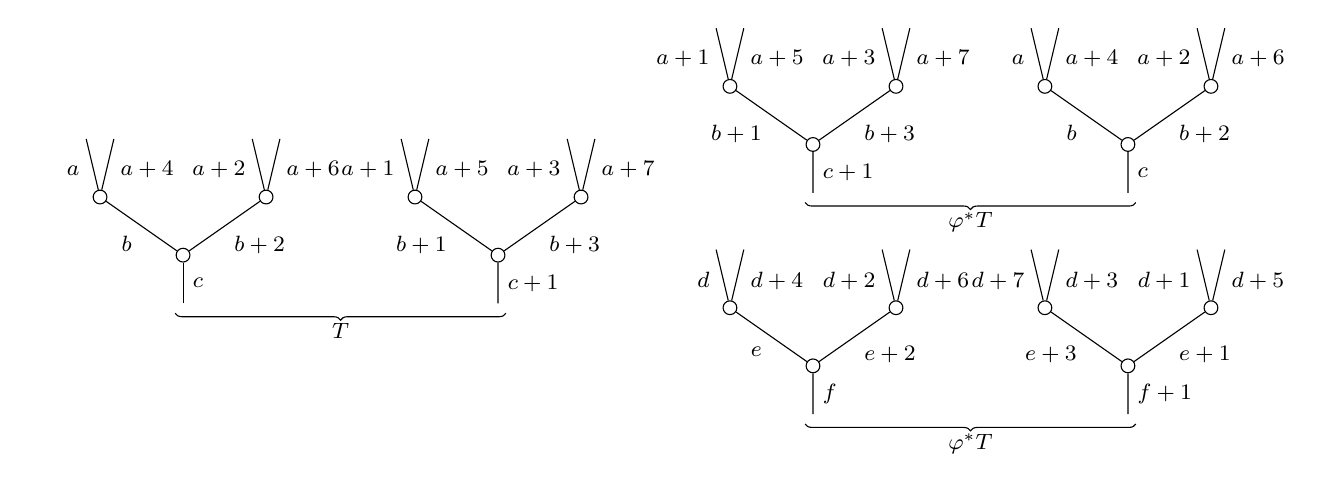
\begin{tikzpicture}[grow=up,auto,level distance=2.1em,every node/.style = {font=\footnotesize},dummy/.style={circle,draw,inner sep=0pt,minimum size=1.75mm}]
		\node at  (0,0) {}
			child{node [dummy] {}
				child[sibling distance = 6em]{node [dummy] {}
					child[sibling distance = 1em]{
					edge from parent node [swap,near end] {$a+6$}}
					child[sibling distance = 1em]{
					edge from parent node [near end] {$a+2$}}
				edge from parent node [swap] {$b+2$}}
				child[sibling distance = 6em]{node [dummy] {}
					child[sibling distance = 1em]{
					edge from parent node [swap,near end] {$a+4$}}
					child[sibling distance = 1em]{
					edge from parent node [near end] {$\phantom{+1}a$}}
				edge from parent node {$b$}}
			edge from parent node [swap] {$c$}};
		\node at  (4,0) {}
			child{node [dummy] {}
				child[sibling distance = 6em]{node [dummy] {}
					child[sibling distance = 1em]{
					edge from parent node [swap,near end] {$a+7$}}
					child[sibling distance = 1em]{
					edge from parent node [near end] {$a+3$}}
				edge from parent node [swap] {$b+3$}}
				child[sibling distance = 6em]{node [dummy] {}
					child[sibling distance = 1em]{
					edge from parent node [swap,near end] {$a+5$}}
					child[sibling distance = 1em]{
					edge from parent node [near end] {$a+1$}}
				edge from parent node {$b+1$}}
			edge from parent node [swap] {$c+1$}};
		\draw[decorate,decoration={brace,amplitude=2.5pt}] (4.1,0) -- (-0.1,0) node[midway]{$T$};
	\begin{scope}[yshift=4em]
		\node at  (12,0) {}
			child{node [dummy] {}
				child[sibling distance = 6em]{node [dummy] {}
					child[sibling distance = 1em]{
					edge from parent node [swap,near end] {$a+6$}}
					child[sibling distance = 1em]{
					edge from parent node [near end] {$a+2$}}
				edge from parent node [swap] {$b+2$}}
				child[sibling distance = 6em]{node [dummy] {}
					child[sibling distance = 1em]{
					edge from parent node [swap,near end] {$a+4$}}
					child[sibling distance = 1em]{
					edge from parent node [near end] {$\phantom{+1}a$}}
				edge from parent node {$b$}}
			edge from parent node [swap] {$c$}};
		\node at  (8,0) {}
			child{node [dummy] {}
				child[sibling distance = 6em]{node [dummy] {}
					child[sibling distance = 1em]{
					edge from parent node [swap,near end] {$a+7$}}
					child[sibling distance = 1em]{
					edge from parent node [near end] {$a+3$}}
				edge from parent node [swap] {$b+3$}}
				child[sibling distance = 6em]{node [dummy] {}
					child[sibling distance = 1em]{
					edge from parent node [swap,near end] {$a+5$}}
					child[sibling distance = 1em]{
					edge from parent node [near end] {$a+1$}}
				edge from parent node {$b+1$}}
			edge from parent node [swap] {$c+1$}};
		\draw[decorate,decoration={brace,amplitude=2.5pt}] (12.1,0) -- (7.9,0) node[midway]{$\varphi^{\**}T$};
	\end{scope}
	\begin{scope}[yshift=-4em]
		\node at  (8,0) {}
			child{node [dummy] {}
				child[sibling distance = 6em]{node [dummy] {}
					child[sibling distance = 1em]{
					edge from parent node [swap,near end] {$d+6$}}
					child[sibling distance = 1em]{
					edge from parent node [near end] {$d+2$}}
				edge from parent node [swap] {$e+2$}}
				child[sibling distance = 6em]{node [dummy] {}
					child[sibling distance = 1em]{
					edge from parent node [swap,near end] {$d+4$}}
					child[sibling distance = 1em]{
					edge from parent node [near end] {$\phantom{+1}d$}}
				edge from parent node {$e$}}
			edge from parent node [swap] {$f$}};
		\node at  (12,0) {}
			child{node [dummy] {}
				child[sibling distance = 6em]{node [dummy] {}
					child[sibling distance = 1em]{
					edge from parent node [swap,near end] {$d+5$}}
					child[sibling distance = 1em]{
					edge from parent node [near end] {$d+1$}}
				edge from parent node [swap] {$e+1$}}
				child[sibling distance = 6em]{node [dummy] {}
					child[sibling distance = 1em]{
					edge from parent node [swap,near end] {$d+3$}}
					child[sibling distance = 1em]{
					edge from parent node [near end] {$d+7$}}
				edge from parent node {$e+3$}}
			edge from parent node [swap] {$f+1$}};
		\draw[decorate,decoration={brace,amplitude=2.5pt}] (12.1,0) -- (7.9,0) node[midway]{$\varphi^{\**}T$};
	\end{scope}
	\end{tikzpicture}
\end{equation}
We note that $(\varphi^{\**}(T))_{v_{G e}} = \psi^{\**}(T_{v_{G b}})$
for $\psi$ the permutation $(13)(24)$ encoded by the composite identifications
$\{1,2,3,4\} \simeq \{e,e+2,e+3,e+1\} \simeq 
\{b+1,b+3,b,b+2\}\simeq \{3,4,1,2\}$.
\end{example}


\begin{lemma}\label{LANPULLCOMA LEM}
	Suppose that $\mathcal{V}$ is complete and that $A \to \Sigma_G$ is a root fibration. If the rightmost triangle in 
	\begin{equation}
	\begin{tikzcd}
		\Omega_{G,0}^{(A)} \ar{r}{V_G^{(A)}} 
		\ar{d} & 
		\Fin \wr A  
		\ar{d}  \ar{r}[swap,name=F]{}&
		\mathcal{V}		
	\\
		\Omega_{G,0} \ar{r}[swap]{V_G} & 
		|[alias=FEG]|\Fin \wr \Sigma_G \ar{ru}
	\arrow[Rightarrow, from=FEG, to=F,shorten <=0.15cm]
	\end{tikzcd}
	\end{equation}
is a right Kan extension diagram then so is the composite diagram.
\end{lemma}


\begin{proof}
	Unpacking definitions using the pointwise formula for right  Kan extensions (\cite[X.3.1]{McL}), 
	it suffices to check that for each $T \in \Omega_{G,0}$ the functor
	\begin{equation}\label{LANPULLCOMA EQ}
	T \downarrow \Omega_{G,0}^{(A)}
	\to 
	V_G(T) \downarrow \Fin \wr A
	\end{equation}
is initial.
In the course of the proof of Lemma \ref{FINWREATPRODLIM LEM}
it was shown that the subcategory
\[
\prod_{v_{Ge} \in V_G(T)} 
T_{v_{Ge}} \downarrow A
\]
is initial in the $V_G(T) \downarrow \Fin \wr A$.

On the other hand, since $\Omega_G^{(A)} \to \Omega_G$ is a root fibration functor, 
$T \downarrow \Omega_{G}^{(A)}$
has an initial subcategory 
$T \downarrow_{\mathsf{r},\simeq} \Omega_{G}^{(A)}$
with objects
$(S \in \Omega_G^{(A)},T \to u(S))$
such that 
$T \to u(S)$
is a quotient map that induces an ordered isomorphism on roots. Note that this can be restated as saying that 
$T \to u(S)$ is an isomorphism preserving the order of the roots.


The result now follows from the natural isomorphism
\begin{equation}\label{TDOWNISOA EQ}
	T \downarrow_{\mathsf{r},\simeq} \Omega_{G}^{(A)} 
\simeq
	\prod_{v_{Ge} \in V_G(T)}
	{T_{v_{Ge}} \downarrow_{\mathsf{r},\simeq} A}.
\end{equation}
To see this, we focus first on the case $A = \Sigma_G$.
In that case, the left hand side of (\ref{TDOWNISOA EQ}) encodes replanarizations of $T$ that preserve the root order.
On the other hand, the right hand side encodes replanarizations of all the $G$-vertices that preserve the order of their roots, or, equivalently, replanarizations of the non-equivariant vertices of $T$.
That these are equivalent is the content of Proposition \ref{PLANARIZATIONCHAR PROP}.

Note that $(T \to S) \in (T \downarrow_{\mathsf{r},\simeq} \Omega_{G})$ is then encoded by a tuple
$\left(T_{v_{Ge}} \to \varphi^{\**}_{v_{Ge}} S_{v_{Ge}}\right)_
{v_{Ge} \in V_G(T)}$
where the pullbacks $\varphi^{\**}_{v_{Ge}}$ are needed to correct the root order.

The case of general $A$ follows likewise, 
using the corresponding pullbacks
$\varphi^{\**}_{v_{Ge}}$.

{\color{red} Note: an addendum is needed to show that (\ref{TDOWNISOA EQ}) suffices, since $T \downarrow_{\mathsf{r},\simeq} \Omega_{G}^{(A)}$ is not sent directly to
 $\prod_{v_{Ge} \in V_G(T)}
	{T_{v_{Ge}} \downarrow_{\mathsf{r},\simeq} A}$}
\end{proof}



Lemma \ref{ROOTFIBPULL LEM} can be interpreted as saying that, if one defines a category
$\mathsf{Wspan}^l_{\mathsf{r}}(\Sigma_G^{op},\mathcal{V})$
of \textit{rooted spans}
\[
\Sigma_G^{op} \leftarrow A^{op} \to \mathcal{V}
\]
where $A \to \Sigma_G$ is a root fibration functor, the monad $N$ built in Proposition \ref{MONSPAN PROP} lifts to a monad 
$N_{\mathsf{r}}$ in
$\mathsf{Wspan}^l_{\mathsf{r}}(\Sigma_G^{op},\mathcal{V})$,
and likewise for the adjunction (\ref{LANIOTAADJ EQ}).

\begin{corollary}
Suppose that finite products in $\mathcal{V}$ commute with colimits in each variable.
The functors
\[
	\mathsf{Lan} \circ N_{\mathsf{r}} \Rightarrow
	\mathsf{Lan} \circ N_{\mathsf{r}} \circ \iota \circ \mathsf{Lan},
\qquad
	\mathsf{Lan} \circ \iota \Rightarrow id
\]
are natural isomorphisms.
\end{corollary}

\begin{proof}
This follows by combining Lemma \ref{LANPULLCOMA LEM} with Lemma \ref{FINWREATPRODLIM LEM}.
\end{proof}


\begin{definition}\label{THEMONAD DEF}
The \textit{genuine equivariant operad monad} is the monad
$\F_G$ on $\mathsf{Fun}(\Sigma_G^{op}, \mathcal{V})$
given by
\[
	\F_G = \mathsf{Lan} \circ N_{\mathsf{r}} \circ \iota
\]
and with multiplication and unit given by the composites
\[
\mathsf{Lan} \circ N_{\mathsf{r}} \circ \iota \circ
\mathsf{Lan} \circ N_{\mathsf{r}} \circ \iota
\overset{\simeq}{\Leftarrow}
\mathsf{Lan} \circ N_{\mathsf{r}} \circ  N_{\mathsf{r}} \circ \iota
\Rightarrow
\mathsf{Lan} \circ N_{\mathsf{r}} \circ \iota
\]
\[
id \overset{\simeq}{\Leftarrow} \mathsf{Lan} \circ \iota
\Rightarrow
\mathsf{Lan} \circ N_{\mathsf{r}} \circ \iota.
\]
\end{definition}


\begin{remark}
	The functor $\mathsf{Lan} \circ N_{\mathsf{r}} \circ \iota$ is isomorphic to 
	$\mathsf{Lan} \circ N \circ \iota$, and this isomorphism is compatible with the multiplication and unit	in Definition \ref{THEMONAD DEF}, and we will henceforth simply write $N$ rather than $N_{\mathsf{r}}$.
	
	From this point of view, the role of root fibrations is to guarantee that $\mathsf{Lan} \circ N \circ \iota$ is indeed a monad, but unnecessary to describe the monad structure itself.
\end{remark}


\begin{remark}\label{REPACKAGERES REM}
Since a map 
\[\F_G X =\mathsf{Lan} \circ N_{\mathsf{r}} \circ \iota X \to X\]
is adjoint to a map
\[N_{\mathsf{r}} \circ \iota X \to \iota X\]
one easily verifies that 
$X$ is a genuine equivariant operad, i.e. 
a $\F_G$-algebra, iff 
$\iota X$ is a $N$-algebra.
Moreover, the bar resolution
\[
	\F_G^{\bullet +1} X 
\]
is isomorphic to
\[
	\mathsf{Lan} \left( N^{\bullet +1} \iota X \right).
\]
\end{remark}


\section{Free extensions}

Our overall goal in this section will be to produce a description of free genuine operad pushouts, i.e. pushouts of the form
\[
\begin{tikzcd}
	\mathbb{F}_G A \ar{r} \ar{d} & X \ar{d}
\\
	\mathbb{F}_G B \ar{r} & Y
\end{tikzcd}
\]
in the category $\mathsf{Op}_G$ of genuine equivariant operads.



\subsection{Extensions over general monads}\label{EXTGENMON SEC}

Any monad $T$ on $\C$ one obtains induced monads $T^{\times l}$ on $\C^{\times l}$, and we will make use of several standard relations between these.
In particular, any map $\alpha \colon \underline{l} \to \underline{m}$ induces a forgetful functor
such that for the forgetul functor 
$\alpha^{\**} \colon \C^{\times l} \to \C^{\times n}$
one has $T^{\times l} \alpha^{\**} \simeq  \alpha^{\**} T^{\times m}$.


Indeed, we will need to make use of a slightly more general setup. Letting $I$ denote the identity monad on $\C$, and $K \subset \underline{m}$ be a subset, there is a monad $T^{\times K} \times I^{\times(\underline{m}-K)}$ on $\mathcal{C}^{\times m}$, which we abusively denote simply as $T^{\times K}$. Identities then determine maps of monads 
$T^{J} \to T^{\times K}$ whenever $J \subset K$
and, moreover, there are identifications
$T^{\times \alpha^{-1}(K)} \alpha^{\**} \simeq \alpha^{\**} T^{\times K}$.
One then has the following.


\begin{proposition}\label{MONADICFUN PROP}
	The functor
\begin{equation}\label{MONADFUNCTORALPHA EQ}
	T^{\times \alpha^{-1} (K)} \Rightarrow \alpha^{\**} T^{\times K} \alpha_{!}
\end{equation}
adjoint to the identification 
$T^{\times \alpha^{-1} (K)} \alpha^{\**} \simeq \alpha^{\**} T^{\times K}$
is a map of monads on $\C^{\times n}$.
\end{proposition}


\begin{proof}
We first note that there are identifications of functors
$(FG)^{\times K} \simeq F^{\times K} G^{\times K}$ which are compatible with the identifications
$F^{\times \alpha^{-1} (K)} \alpha^{\**} \simeq \alpha^{\**} F^{\times K}$
in the sense that the identification
$(F G)^{\times \alpha^{-1} (K)} \circ \alpha^{\**} \simeq 
\alpha^{\**} (FG)^{\times K}$
matches the composite identification
$F^{\times \alpha^{-1} (K)} G^{\times \alpha^{-1} (K)} \alpha^{\**} \simeq
F^{\times \alpha^{-1} (K)}\alpha^{\**}G^{\times K} \simeq
\alpha^{\**} F^{\times K} G^{\times K}$.

Letting $\eta, \epsilon$ denote the unit and counit for the 
$(\alpha_{!},\alpha^{\**})$ adjunction, 
(\ref{MONADFUNCTORALPHA EQ})
is then the composite
\[
	T^{\times \alpha^{-1} (K)} \xrightarrow{\eta} 
	T^{\times \alpha^{-1} (K)} \alpha^{\**} \alpha_{!} \simeq
	\alpha^{\**} T^{\times K}\alpha_{!}.
\]
That this is a monad map is the condition that the following multiplication and unit diagrams commute.
\[
\begin{tikzcd}
	T^{\times \alpha^{-1} (K)} \circ T^{\times \alpha^{-1} (K)} \ar{d} \ar{r} &
	\alpha^{\**} T^{\times K} \alpha_{!} \circ 
	\alpha^{\**} T^{\times K} \alpha_{!} \ar{d} &
	I^{\times n} \ar{d} \ar{rd}& 	
\\
	T^{\times \alpha^{-1} (K)} \ar{r} &
	\alpha^{\**} T^{\times K} \alpha_{!} &
	T^{\times \alpha^{-1} (K)} \ar{r} &
	\alpha^{\**} T^{\times K} \alpha_{!}
\end{tikzcd}
\]
We argue only the case of the leftmost multiplication diagram, with commutativity of the unit diagram following by a similar but simpler argument. Since the precomposition
$(\minus) \circ \alpha^{\**}$
is the left adjoint to the precomposition
$(\minus) \circ \alpha_{!}$
this follows from the following diagram.
\[
\begin{tikzcd}
	T^{\times \alpha^{-1} (K)}  T^{\times \alpha^{-1} (K)}  \alpha^{*} \ar{r}{\simeq} \ar{dd}&
	T^{\times \alpha^{-1} (K)}  \alpha^{*}  T^{\times K} \ar{r}{\eta}
	\ar[equal]{rd} &
	T^{\times \alpha^{-1} (K)} \alpha^{\**} \alpha_{!} \alpha^{*} T^{\times K} \ar{d}{\epsilon} \ar{r}{\simeq}&
	\alpha^{\**} T^{\times K} \alpha_{!} \alpha^{\**}  T^{\times K} \ar{d}{\epsilon}
\\
	& &
	T^{\times \alpha^{-1} (K)}  \alpha^{*}  T^{\times K} \ar{r}{\simeq} &
	\alpha^{*}  T^{\times K}  T^{\times K} \ar{d}
\\
	T^{\times \alpha^{-1} (K)}  \alpha^{*} \ar{rrr}{\simeq} &&&
	\alpha^{*} T^{\times K}
\end{tikzcd}
\]
\end{proof}


\begin{remark}\label{TALPHAKMOD REM}
	Since $T^{\times K} \alpha_{!}$ is a right 
	$\alpha^{\**} T^{\times K}\alpha_{!}$-module,
	Proposition \ref{MONADICFUN PROP} implies that it is also a 
	right $T^{\times \alpha^{-1}(K)}$-module or, moreover, a 
	right $T^{\times J}$-module whenever $\alpha(J) \subset K$.
\end{remark}


\begin{remark}\label{PRECOMPPOSTCOMP REM}
Combining the precomposition and postcomposition adjunctions,
the identification 
$T^{\times \alpha^{-1} (K)} \alpha^{\**} \simeq \alpha^{\**} T^{\times K}$
is then adjoint to a functor
$	\alpha_{!} T^{\times \alpha^{-1} (K)} 
	\to
	T^{\times K} \alpha_{!}$
which is readily checked to be a map of right $T^{\times \alpha^{-1} (K)}$-modules.

More generally, for $\alpha(J) \subset K$, the composite 
$T^{\times J}\alpha^{\**} \to T^{\times \alpha^{-1} (K)} \alpha^{\**} \simeq \alpha^{\**} T^{\times K}$ is thus adjoint to a map of right $T^{\times J}$-modules
\begin{equation}\label{RIGHTMODULETMAP EQ}
	\alpha_{!} T^{\times J} \to T^{\times K} \alpha_{!}.
\end{equation}
We now unpack the content of (\ref{RIGHTMODULETMAP EQ}) when 
$\alpha \colon \underline{l} \to \**$ is the unique map to the simpleton $\** = \underline{1}$. In this case we can instead write $\alpha_{!} = \coprod$, $\alpha^{\**}=\Delta$,
and we thus have commutative diagrams
\begin{equation}\label{RIGHTMODULETMAPAUX EQ}
\begin{tikzcd}
	\coprod_{J} TT A_j \amalg \coprod_{\underline{n}-J} A_j
	\ar{r} \ar{d} &
	T\left( \coprod_{J} T A_j \amalg \coprod_{\underline{n}-J} A_j \right) \ar{d}
\\
	\coprod_{J} T A_j \amalg \coprod_{\underline{n}-J} A_j
	\ar{r} &
		T\left( \coprod_{J} A_j \amalg \coprod_{\underline{n}-J} A_j \right)
\end{tikzcd}
\end{equation}
where the vertical maps
come from the right $T^{\times J}$-module structure.
Writing $\amalg^a$ for the coproduct of $T$-algebras and recalling the canonical identifications 
$\coprod^a_K (T A_k) \simeq T\left( \coprod_K A_k \right)$, 
(\ref{RIGHTMODULETMAPAUX EQ}) in fact shows that the 
right $T^{\times J}$-module structure on $T \circ \coprod$
in fact codifies the multiplication maps
\[
\coprod^a_J TT A_j \amalg^a \coprod^a_{\underline{l}-J} T A_j
	\to
\coprod^a_J T A_j \amalg^a \coprod^a_{\underline{l}-J} T A_j.
\] 
\end{remark}


\subsection{Labeled planar strings}

We now translate the results in the previous section to the context of the monad $N$ on $\mathsf{WSpan}^l(\Sigma^{op},\mathcal{V})$. In analogy to the planar string models $\Omega_{G,n}^{(A)}$ for iterations $N^{\circ n+1}$ of the monad $N$,
we will find it convenient to build similar string models
$\Omega_{G,n}^{(\underline{A}_J)}$ for 
$N \circ \coprod \circ (N^{\times J})^{\circ n}$.


\begin{definition}
A \textit{$l$-node labeled $G$-tree} (or just \textit{$l$-labeled $G$-tree}) $G$-tree is a pair $(T,V_G(T) \to \{1,\cdots,l\})$ with $T \in \Omega_G$, which we think of as a $G$-tree together with $G$-vertices labels in $1,\cdots,l$.

Further, a tall map $\varphi \colon T \to S$ between $l$-labeled trees is called a \textit{label map} if for each $G$-vertex $v_{G e}$ of $T$ with label $j$, the vertices of the subtree $S_{v_{G e}}$ are all labeled by $j$.

Lastly, given a subset $J\subset \underline{l}$, a planar label map $\varphi \colon T \to S$ is said to be $J$-inert if for every $G$-vertex $v_{G e}$ of $T$ with label $j \in J$ it is $S_{v_{Ge}} = T_{v_{Ge}}$.
\end{definition}


\begin{example}\label{LABELEDTREES EX}
Consider the $2$-labeled trees below (for $G=\**$ the trivial group), with black nodes ($\bullet$) denoting labels by the number $1$ and white nodes ($\circ$) labels by the number $2$.
The planar map $\varphi$ (sending $a_i\mapsto a$, 
$b \mapsto b$, $c \mapsto c$, $d \mapsto d$, $e \mapsto e$) is a label map which is $\{1\}$-inert.
\begin{equation}\label{SUBSDATUMTREESLAB EQ}
	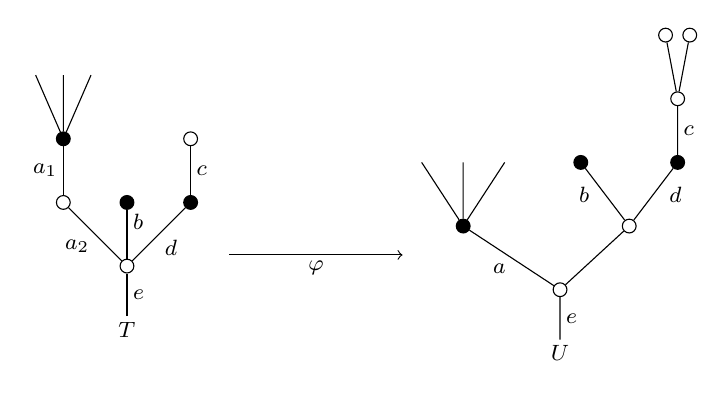
\begin{tikzpicture}[grow=up,auto,level distance=2.1em,
	every node/.style = {font=\footnotesize,inner sep=2pt},
	dummy/.style={circle,draw,inner sep=0pt,minimum size=1.75mm}]
	\begin{scope}[level distance=2.3em]
	\tikzstyle{level 2}=[sibling distance=3.5em]%
	\tikzstyle{level 3}=[sibling distance=2.25em]%
	\tikzstyle{level 4}=[sibling distance=1.25em]%
	\tikzstyle{level 5}=[sibling distance=0.875em]%
		\node at (5.5,0) {$U$}
			child{node [dummy] {}
				child[sibling distance =5em]{node [dummy] {}
					child[sibling distance =3.5em]{node [dummy,fill=black] {}
						child{node [dummy] {}
							child{node [dummy] {}}
							child{node [dummy] {}}
						edge from parent node [swap] {$c$}}
					edge from parent node [swap, near end] {$d$}}
					child[sibling distance =3.5em]{node [dummy,fill=black] {}
					edge from parent node [near end] {$b$}}
				}
				child[sibling distance =7em]{node [dummy,fill=black] {}
					child[sibling distance =1.5em]
					child[sibling distance =1.5em]
					child[sibling distance =1.5em]
				edge from parent node {$a$}}
			edge from parent node [swap] {$e$}};
	\end{scope}
	\begin{scope}[level distance=2.3em]
	\tikzstyle{level 2}=[sibling distance=2.3em]%
	\tikzstyle{level 4}=[sibling distance=1em]%
		\node at (0,0.3) {$T$}
			child{node [dummy] {}
				child{node [dummy,fill=black] {}
					child{node [dummy] {}
					edge from parent node [swap] {$c$}}	
				edge from parent node [swap] {$d$}}
				child{node [dummy,fill=black] {}
				edge from parent node [near end,swap] {$b$}}
				child{node [dummy] {}
					child{node [dummy,fill=black] {}
						child
						child
						child
					edge from parent node {$a_1$}}
				edge from parent node {$a_2$}}
			edge from parent node [swap] {$e$}};
	\end{scope}
	\draw [->] (1.3,1.25) -- node[swap] {$\varphi$} (3.5,1.25);
	\end{tikzpicture}
\end{equation}
\end{example}



\begin{definition}
Let $0 \leq s \leq n$ and $J \subset \underline{l}$ be a subset.

We define $\Omega_{G,n,s}^{J}$ to have as objects $n$-planar strings
\begin{equation}\label{NSTRINGLAB EQ}
	T_0 \xrightarrow{f_1}
	T_1 \xrightarrow{f_2}
	\cdots \xrightarrow{f_s}
	T_s \xrightarrow{f_{s+1}}
	T_{s+1} \xrightarrow{f_{s+2}}
	\cdots \xrightarrow{f_n}
	T_{n}
\end{equation}
together with
$l$-labelings of $T_s, T_{s+1},\cdots, T_{n}$ such that the $f_r,r>s$ are $(\underline{l}-J)$-inert label maps.

Arrows in $\Omega_{G,n,s}^{J}$ are quotients of strings 
$(q_r \colon T_r \to T'_r)$ such that 
$q_r,r\leq s$ are label maps.
\end{definition}

Informally, $\Omega_{G,n,s}^{\underline{l}}$ consists of $n$-strings such that trees and maps after $T_s$ are $l$-labeled.

\begin{remark} 
Our main case of interest will that of $s=0$, in which case we abbreviate 
$\Omega_{G,n}^{J} = \Omega_{G,n,0}^{J}$.
Indeed, such strings will suffice to build models for $N \circ \coprod \circ (N^{\times J})^{\circ n}$.

However, to unpack the right $N^{\times J}$-module structure as in Remark \ref{TALPHAKMOD REM} one further needs to encode composites $NN \circ \coprod \circ (N^{\times J})^{\circ n-1}$, 
a role played by strings $\Omega_{G,n,1}^{J}$.
\end{remark}

\begin{notation}
	We will further write 
\begin{equation}\label{OMEGANMINUSONE EQ}
	\Omega_{G,n,-1}^{J} = \coprod_J \Omega_{G,n} \amalg \coprod_{\underline{l}-J} \Sigma_G,
	\qquad
	\Omega_{G,n,n+1}^{J} = \Omega_{G,n}
\end{equation}
To justify this convention, we note that a string as in (\ref{NSTRINGLAB EQ}) can be extended by prepending to it the map $\mathsf{lr}(T_0) = T_{-1} \xrightarrow{f_0} T_0$. If one then attempts to define $\Omega_{G,n,-1}^{J}$ by insisting that  $T_{-1}$ also be labeled, it follows that all node labels in each string must coincide, resulting in the coproduct decomposition in (\ref{OMEGANMINUSONE EQ}).
\end{notation}


There are a number of obvious functors relating the $\Omega_{G,n,s}^{J}$ categories, which we now make explicit.
Given $s\leq s'$ or $J \subset J'$ there are forgetful functors
\begin{equation}\label{NKNFGT EQ}
	\Omega_{G,n,s}^{J} \to \Omega_{G,n,s'}^{J}
\qquad
	\Omega_{G,n,s}^{J} \to \Omega_{G,n,s}^{J'}
\end{equation}
The simplicial operators in Notation \ref{SIMPOPERATORS NOT}
generalize to operators (where $0 \leq i \leq n$, $-1\leq j \leq n$)
\[
\begin{tikzcd}[row sep =0,column sep =1em]
	d_i \colon 
	\Omega_{G,n,s}^{J} \ar{r} &
	\Omega_{G,n-1,s-1}^{J} &
	i < s & & & &
	s_j \colon 
	\Omega_{G,n,s}^{J} \ar{r} &
	\Omega_{G,n+1,s+1}^{J} &
	j < s
\\
	d_i \colon 
	\Omega_{G,n,s}^{J} \ar{r} &
	\Omega_{G,n-1,s}^{J} &
	s \leq i & & & &
	s_j \colon 
	\Omega_{G,n,s}^{J} \ar{r} &
	\Omega_{G,n+1,s}^{J} &
	s \leq j
\end{tikzcd}
\]
which are compatible with the forgetful functors in the obvious way.


\begin{remark}
	For $J \subset J'$ the forgetful functor in (\ref{NKNFGT EQ}) is a fully faithful inclusion. 
	However, and somewhat subtly, this is not the case the for the $ s \leq s'$ forgetful functors. Indeed, regarding
	$T \to U$ in Examples \ref{LABELEDTREES EX} as an object in 
	$\Omega_{\**,n,0}^{\underline{2}}$, changing the label of the $a_1 \leq a_2$ vertex of $T$ from a $\circ$-label to a $\bullet$-label yields an alternate object $\bar{T} \to U$
	of $\Omega_{\**,n,0}^{\underline{2}}$ forgetting to the same object of $\Omega_{\**,n,1}^{\underline{2}}$, yet $T \to U$ and $\bar{T} \to U$ are not isomorphic.
	
	We note that this is a consequence of the fact that substitution data can replace unary nodes by stumps, which have no nodes.
\end{remark}

Generalizing Notation \ref{INDVNG NOT} there is a commutative diagram 
\[
\begin{tikzcd}
	\Omega_{G,n,s}^{J} \ar{r}{V_{G,n}} \ar{d}& 
	\Fin \wr \Sigma_G^{\amalg l} \ar{d}
\\
	\Omega_{G,n} \ar{r}[swap]{V_{G,n}} &
	\Fin \wr \Sigma_G
\end{tikzcd}
\]
where for a labeled string it is 
$V_G(T_0 \to \cdots \to T_n) =
(T_{n,v_{Ge}})_{V_G(T_n)}$, where we regard 
$T_{n,v_{Ge}} \in \Sigma_G^{\amalg l} \simeq \Omega_{G,-1,-1}^{\underline{l}}$ by using the label in $1,\cdots, l$.

We now expand Notation \ref{OMEGAGNA NOT}.

\begin{notation}
	Let $\underline{A}$ denote a $\underline{l}$-tuple 
	$(\pi_j \colon A_j \to \Sigma_G)_{\underline{l}}$ of categories over $\Sigma_G$. We define $\Omega_{G,n,s}^{(\underline{A}),J}$ by the pullback diagram
\begin{equation}\label{LTUPLEAPULL EQ}
\begin{tikzcd}
	\Omega_{G,n,s}^{(\underline{A}),J} \ar{r}{V_{G,n}^{(\underline{A})}} \ar{d}& 
	\Fin \wr \coprod A_j \ar{d}
\\
	\Omega_{G,n,s}^{J} \ar{r}[swap]{V_{G,n}} & 
	\Fin \wr \Sigma_G^{\amalg l} 
\end{tikzcd}
\end{equation}
Explicitly, an object of $\Omega_{G,n,s}^{(\underline{A}),J}$ consists of a labeled string $T_0 \to \cdots T_n$ as in (\ref{NSTRINGLAB EQ})
together with 
a tuple $(a_{v_{Ge}})_{V_G(T_n)}$ such that
$a_{v_{Ge}} \in A_j$ if $v_{Ge}$ has label $j$ and 
$\pi_j (a_{v_{Ge}}) = T_{n,v_{Ge}}$.
\end{notation}


The reader may have noticed a certain asymmetry between our definition of the $V_{G,n}$ functors here versus their analogues in \S \ref{PLANARSTRING SEC}, where they were defined iteratively in terms of simpler functors $V_G$. This is because of the possibility that $s=-1$, in which case (\ref{OMEGANMINUSONE EQ}) applies and some caution is needed in that the following result fails.


\begin{proposition}\label{ALLSQUARESJ PROP}
Suppose $0\leq s \leq n$. One has a diagram of pullback squares
(generalizing (\ref{ALLSQUARES EQ}))
\begin{equation}\label{ALLSQUARESJ EQ}
\begin{tikzcd}[column sep = 3em]
	\Omega^{(\underline{A}),J}_{G,n,s} \ar{r}{V_G^{(A)}} \ar{d}& 
	\Fin \wr \Omega^{(\underline{A}),J}_{G,n-1,s-1} \ar{r}{\Fin \wr V_{G,n}^{(A)}} \ar{d}&
	\Fin \wr \Fin \wr \coprod A_j  \ar{d} \ar{r}{\sigma^0} &
	\Fin \wr \coprod A_j \ar{d}
\\
	\Omega_{G,n,s}^J \ar{r}{V_G} \ar{d} &
	\Fin \wr \Omega_{G,n-1,s-1}^J \ar{r}{\Fin \wr V_{G,n}} \ar{d} &
	\Fin \wr \Fin \wr \Sigma_G^{\amalg l} \ar{r}{\sigma^0} &
	\Fin \wr \Sigma_G^{\amalg l}
\\
	\Omega_{G,0} \ar{r}{V_G} &
	\Fin \wr \Sigma_G
\end{tikzcd}
\end{equation}
such that the composite of the top squares is (\ref{LTUPLEAPULL EQ}).
\end{proposition}


\begin{proof}
	The $V_G$ functors are defined just as in (\ref{VGDEF EQ}) via the formula
	\[
	V_G(T_0 \to T_1 \to \cdots \to T_n) = 
	(T_{1,v_{Ge}} \to \cdots \to
	T_{n,v_{Ge}})_{v_{Ge} \in V_G(T_0)}\]
with the strings 
$T_{1,v_{Ge}} \to \cdots \to T_{n,v_{Ge}}$
inheriting the extra structure in the obvious way.

Since the top composite square, top center square and top right square are all pullback squares, it remains only to show that the bottom left square is a pullback.
This last claim is simply a variation of Proposition \ref{SUBSASPULL PROP}, and follows from the same proof, since both labels and inertness conditions are inherited when assembling substitution data into trees via Proposition \ref{SUBDATAUNDERPLAN PROP}.
\end{proof}


\subsection{Bar constructions on spans}

We use the results in the previous sections to obtain a string description of the bar constructions
\[
\coprod_J^a N^{\bullet +1} A_j \amalg^a
\coprod_{\underline{l}-J}^a N A_j.
\]

For simplicity, we discuss first the particular case 
$\coprod^a N^{\bullet +1} A$. Writing the span as 
$\Sigma_G \leftarrow A \xrightarrow{F} \mathcal{V}$
the identifications 
$\Omega_{G,0}^{\left( \Omega_{G,n}^{(A)} \right)} \simeq \Omega_{G,n+1}^{(A)}$
iteratively identify the operator in the bar construction
$N^{\bullet+1} A$ as follows.

The top boundaries $d_n$ have natural transformation given by
\begin{equation}
	\begin{tikzcd}[column sep=3.7em]
	\Omega_{G,n}^{(A)} \ar{d} \ar{r}{V_G^{\circ n}} &
	\Fin^{\wr n} \wr \Omega_{G,0}^{(A)} \ar{r}{\Fin^{\wr n}\wr F_1} \ar{d}&
	|[alias=dog2]|
	\Fin^{\wr n} \wr \mathcal{V}^{op} \ar{r}{\Pi^{\circ n}}  \ar[equal]{d} &
	\mathcal{V}^{op} \ar[equal]{d}
\\
	\Omega_{G,n-1}^{(A)} \ar{r}[swap]{V_G^{\circ n}} &
	|[alias=cat3]|
	\Fin^{\wr n} \wr A \ar{r}[swap]{\Fin^{\wr n} \wr F} &
	\Fin^{\wr n} \wr \mathcal{V}^{op} \ar{r}[swap]{\Pi^{\circ n}} &
	|[alias=dog]|
	\mathcal{V}^{op}
	\arrow[Rightarrow, from=dog2, to=cat3,shorten <=0.15cm,,shorten >=0.15cm,"\Fin^{\wr n} \wr m"]
	\end{tikzcd}
\end{equation}
where $m$ is the natural transformation component of the multiplication $NA \to A$, and the remaining differentials
$d_i$ for $0 \leq i < n$ are given by
\begin{equation}\label{REMAINDIFF EQ}
	\begin{tikzcd}[column sep=3.7em]
	\Omega_{G,n}^{(A)} \ar{d}[swap]{d_i^{(A)}} \ar{r}{V_G^{\circ n + 1}} &
	|[alias=dog2]|
	\Fin^{\wr n+1} \wr A \ar{r}{F} \ar{d}{\sigma^i}&
	\Fin^{\wr n+1} \wr \mathcal{V}^{op} \ar{r}{\Pi^{\circ n+1}}  \ar{d}{\sigma^i} &
	|[alias=dog3]|
	\mathcal{V}^{op} \ar[equal]{d}
\\
	|[alias=cat2]|
	\Omega_{G,n-1}^{(A)} \ar{r}[swap]{V_G^{\circ n}} &
	\Fin^{\wr n} \wr A \ar{r}[swap]{F} &
	|[alias=cat3]|
	\Fin^{\wr n} \wr \mathcal{V}^{op} \ar{r}[swap]{\Pi^{\circ n}} &
	|[alias=dog]|
	\mathcal{V}^{op}
	\arrow[Leftrightarrow, from=dog2, to=cat2,shorten <=0.15cm,,shorten >=0.15cm,"\pi_i^{(A)}"]
	\arrow[Leftrightarrow, from=dog3, to=cat3,shorten <=0.15cm,,shorten >=0.15cm,"\alpha_i"]
	\end{tikzcd}
\end{equation}
where $\pi_i^{(A)}$ interchanges lexicographic orders on the $i$-th $\Fin$ coordinate of $F^{\wr n}$ and $\alpha_i$ is the natural associativity isomorphism.

{\color{blue} Maybe add degeneracies}

Similarly, Proposition \ref{ALLSQUARESJ PROP} shows that
$\Omega_{G,n}^{(A)} \simeq
\Omega_{G,0}^{\left( \coprod \Omega_{G,n-1}^{(A_j)} \right)}$
so that the top boundaries $d_n$ in the bar construction
$N \circ \amalg \circ (N^{\times l})^{\circ n} \underline{A}$
are given by
\begin{equation}
	\begin{tikzcd}[column sep=2em]
	\Omega_{G,n}^{(\underline{A})} \ar{d} \ar{r}{V_G} &
	\Fin \wr \coprod \Omega_{G,n-1}^{(A_j)} \ar{r}{V_G^{\circ n-1}}&
	\Fin \wr \coprod \Fin^{\wr n-1} \wr \Omega_{G,0}^{(A_j)} \ar{r}{F_1} \ar{d}&
	|[alias=dog2]|
	\Fin \wr \coprod \Fin^{\wr n-1} \wr \mathcal{V}^{op} \ar{r}{\Pi^{\circ n-1}}  \ar[equal]{d} &
	\Fin \wr \mathcal{V}^{op} \ar{r}{\Pi} &
	\mathcal{V}^{op} \ar[equal]{d}
\\
	\Omega_{G,n-1}^{(\underline{A})} \ar{r}[swap]{V_G} &
	\Fin \wr \coprod \Omega_{G,n-2}^{(A_j)} \ar{r}[swap]{V_G^{\circ n-1}}&
	|[alias=cat3]|
	\Fin \wr \coprod \Fin^{\wr n-1} \wr A_j \ar{r}[swap]{F} &
	\Fin \wr \coprod \Fin^{\wr n-1} \wr \mathcal{V}^{op} \ar{r}[swap]{\Pi^{\circ n-1}} &
	\Fin \wr \mathcal{V}^{op} \ar{r}[swap]{\Pi} &
	|[alias=dog]|
	\mathcal{V}^{op}
	\arrow[Rightarrow, from=dog2, to=cat3,shorten <=0.15cm,,shorten >=0.15cm,"\underline{m}"]
	\end{tikzcd}
\end{equation}
where $\underline{m}$ stands for the functor induced by the tuple of multiplication maps $m_j \colon N A_j \to A_j$, 
and the other boundaries $d_i$ for $0 \leq i < n$ are given by
\begin{equation}\label{DISJBARDN EQ}
	\begin{tikzcd}[column sep=2em,row sep=3em]
	\Omega_{G,n}^{(\underline{A})} 
	\ar{d}[swap]{d_i^{(\underline{A})}} \ar{r}{V_G} &
	\Fin \wr \coprod \Omega_{G,n-1}^{(A_j)} \ar{r}{V_G^{\circ n}} &
	|[alias=dog2]|
	\Fin \wr \coprod \Fin^{\wr n} \wr A \ar{r}{F} \ar{d}{\sigma^i}&
	\Fin \wr \coprod \Fin^{\wr n} \wr \mathcal{V}^{op} \ar{r}{\Pi^{\circ n}}  \ar{d}{\sigma^i} &
	\Fin \wr \mathcal{V}^{op} \ar{r}{\Pi} &
	|[alias=dog3]|
	\mathcal{V}^{op} \ar[equal]{d}
\\
	|[alias=cat3]|
	\Omega_{G,n-1}^{(\underline{A})} \ar{r}[swap]{V_G} &
	\Fin \wr \coprod \Omega_{G,n-2}^{(A_j)} \ar{r}[swap]{V_G^{\circ n-1}}&
	\Fin \wr \coprod \Fin^{\wr n-1} \wr A \ar{r}[swap]{F} &
	|[alias=cat2]|
	\Fin \wr \coprod \Fin^{\wr n-1} \wr \mathcal{V}^{op} \ar{r}[swap]{\Pi^{\circ n-1}} &
	\Fin \wr \mathcal{V}^{op} \ar{r}[swap]{\Pi} &
	\mathcal{V}^{op}
	\arrow[Leftrightarrow, from=dog2, to=cat3,shorten <=0.15cm,,shorten >=0.15cm,"\pi_i^{(\underline{A})}"]
	\arrow[Leftrightarrow, from=dog3, to=cat2,shorten <=0.15cm,,shorten >=0.15cm,"\alpha_i"]
	\end{tikzcd}
\end{equation}
where again $\pi_i^{(\underline{A})}$ interchanges lexicographic orders on the $i$-th $\Fin$ coordinate and $\alpha_i$ is again an associativity isomorphism.
We note that (\ref{DISJBARDN EQ}) follows directly from 
(\ref{REMAINDIFF EQ}) for $0<i<n$, but that the case $i=0$, which uses the $N^{\times l}$ right action on $N \circ \amalg$ (cf. Remark \ref{TALPHAKMOD REM}), which after unpacked leads to the composite diagram below.
\begin{equation}\label{ASSOCSPANJ1 EQ}
	\begin{tikzcd}[column sep=0.5em]
	\Omega_{G,n}^{(\underline{A})}  \ar{d} \ar{r} &
	\Fin \wr \coprod \Omega_{G,n-1}^{(A_j)} \ar{d} \ar{rr} &&
	\Fin \wr \coprod \Fin^{\wr n-1} A_j \ar{d} \ar{r}&
	\Fin \wr \coprod \Fin^{\wr n-1} \mathcal{V}^{op} \ar{d}\ar{rr} & &
	|[alias=cat3]|
	\Fin \wr \mathcal{V}^{op} \ar[equal]{d} \ar{r} &
	\mathcal{V}^{op} \ar[equal]{d}
\\
	\Omega_{G,n,1}^{(\underline{A})} \ar{r} \ar{d}[swap]{d_0^{(\underline{A}}} &
	|[alias=cat2]|
	\Fin \wr \Omega_{G,n-1}^{(\underline{A})} \ar{r} &
	|[alias=FFOmega]| \Fin^{\wr 2} \wr \coprod \Omega_{G,n-2}^{(A_j)} \ar{d}{\sigma^0} \ar{r} &
	\Fin^{\wr 2} \wr \coprod \Fin^{\wr n-2} A_j \ar{d}{\sigma^0} \ar{r} &
	\Fin^{\wr 2} \wr \coprod \Fin^{\wr n-2} \mathcal{V}^{op} \ar{d}{\sigma^0} \ar{r}&
	|[alias=dog3]|
	\Fin^{\wr 2} \wr \mathcal{V}^{op} \ar{d}{\sigma^0} \ar{r} &
	\Fin \wr \mathcal{V}^{op} \ar{r} &
	|[alias=dog]|
	\mathcal{V}^{op} \ar[equal]{d}
\\
	|[alias=Omega]|\Omega_{G,n-1}^{(\underline{A})} \ar{rr} &&
	\Fin \wr \coprod \Omega_{G,n-2}^{(A_j)} \ar{r} &
	\Fin \wr \coprod \Fin^{\wr n-2} A_j \ar{r} &
	\Fin \wr \coprod \Fin^{\wr n-2} \mathcal{V}^{op} \ar{r}&
	|[alias=cat]|
	\Fin \wr \mathcal{V}^{op} \ar{rr} &&
	\mathcal{V}^{op}
	\arrow[Leftrightarrow, from=FFOmega, to=Omega,shorten <=0.15cm,shorten >=0.15cm,"\pi_0"]
	\arrow[Leftrightarrow, from=dog, to=cat,shorten <=0.15cm,shorten >=0.15cm,"\alpha_0"]
	\end{tikzcd}
\end{equation}
%Note: the top section can be factored by
%\[
%\begin{tikzcd}
%	\coprod \Omega_{n+1}^{(A_j)} \ar{r} \ar{d}&
%	\coprod \Fin \wr \Omega_{n}^{(A_j)} \ar{d}
%\\
%	\coprod \Omega_{n+1}^{(\underline{A})} \ar{r} \ar{d} &
%	\coprod \Fin \wr \coprod \Omega_{n}^{(A_j)} \ar{d}
%\\
%	\Omega_{n+1}^{(\underline{A})} \ar{r} &
%	\Fin \wr \coprod \Omega_{n}^{(A_j)}
%\end{tikzcd}
%\]
Finally, using the inclusions $\Omega_{G,n}^{(\underline{A}),J} \hookrightarrow \Omega_{G,n}^{(\underline{A})}$,
one obtains analogous descriptions of the bar constructions 
$N \circ \amalg \circ (N^{\times J})^{\circ n} \underline{A}$, 
depicted below.
\begin{equation}
	\begin{tikzcd}[column sep=2em]
	\Omega_{G,n}^{(\underline{A}),J} \ar{d} \ar{r} &
	\Fin \wr \left( \coprod_J \Fin^{\wr n-1} \wr \Omega_{G,0}^{(A_j)} 
	\amalg \coprod_{\underline{l}-J} A_j \right)
	\ar{r}{F_1} \ar{d}&
	|[alias=dog2]|
	\Fin \wr \coprod \Fin^{\wr n-1} \wr \mathcal{V}^{op} \ar{r}  \ar[equal]{d} &
	\mathcal{V}^{op} \ar[equal]{d}
\\
	\Omega_{G,n-1}^{(\underline{A}),J} \ar{r} &
	|[alias=cat3]|
	\Fin \wr \left( \coprod_J \Fin^{\wr n-1} \wr A_j
	\amalg \coprod_{\underline{l}-J} A_j \right)
	\ar{r}[swap]{F} &
	\Fin \wr \coprod \Fin^{\wr n-1} \wr \mathcal{V}^{op} \ar{r} &
	\mathcal{V}^{op}
	\arrow[Rightarrow, from=dog2, to=cat3,shorten <=0.15cm,,shorten >=0.15cm,"\underline{m}"]
	\end{tikzcd}
\end{equation}

\begin{equation}\label{DISJBARDNJ EQ}
	\begin{tikzcd}[column sep=2em,row sep=3em]
	\Omega_{G,n}^{(\underline{A}),J} 
	\ar{d}[swap]{d_i^{\underline{A}}} \ar{r} &
	|[alias=dog2]|
	\Fin \wr \left( \coprod_J \Fin^{\wr n} \wr A_j 
	\amalg \coprod_{\underline{l}-J} A_j \right)
	\ar{r}{F} \ar{d}{\sigma^i}&
	\Fin \wr \coprod \Fin^{\wr n} \wr \mathcal{V}^{op} \ar{r}  \ar{d}{\sigma^i} &
	|[alias=dog3]|
	\mathcal{V}^{op} \ar[equal]{d}
\\
	|[alias=cat3]|
	\Omega_{G,n-1}^{(\underline{A}),J} \ar{r} &
	\Fin \wr \left( \coprod_J \Fin^{\wr n-1} \wr A_j
	\amalg \coprod_{\underline{l}-J} A_j \right) \ar{r}[swap]{F} &
	|[alias=cat2]|
	\Fin \wr \coprod \Fin^{\wr n-1} \wr \mathcal{V}^{op} \ar{r} &
	\mathcal{V}^{op}
	\arrow[Leftrightarrow, from=dog2, to=cat3,shorten <=0.15cm,,shorten >=0.15cm,"\pi_i^{(\underline{A})}"]
	\arrow[Leftrightarrow, from=dog3, to=cat2,shorten <=0.15cm,,shorten >=0.15cm,"\alpha_i"]
	\end{tikzcd}
\end{equation}


\subsection{Transferring simplicial colimits of left Kan extensions} \label{TRANSFSIMP SEC}


Given genuine equivariant operads 
$X,Y \in \mathsf{Op}_G$
one has an isomorphism
\[
	X \amalg^a Y 
\simeq
	\colim_{\Delta^{op}} 
	\left(
	\mathbb{F}_G^{\bullet+1} X \amalg^a \mathbb{F}_G^{\bullet+1} Y
	\right)
\]
so that combining Remarks \ref{REPACKAGERES REM}
and
Remark \ref{PRECOMPPOSTCOMP REM}
with the results in the previous section one obtains isomorphisms
\begin{align}
	X \amalg^a Y  
\simeq &
	\colim_{\Delta^{op}} 
	\left(
	\mathsf{Lan} \left(
	N^{\bullet+1} \iota X \amalg^a N^{\bullet+1} \iota Y
	\right) \right)
\\
\simeq &
	\colim_{\Delta^{op}} 
	\left(
	\mathsf{Lan} \left(
	N \circ \amalg \circ (N^{\times 2})^{\bullet} (\iota X,\iota Y)
	\right) \right)
\\ \label{COLIMLAN EQ}
\simeq &
	\colim_{\Delta^{op}} 
	\left(
	\mathsf{Lan}_{\Omega_{G,\bullet}^{\underline{2},op} \to \Sigma_G^{op}}
	N_{\bullet}^{(X,Y)}
	\right)
\end{align}
where we write 
$N_{\bullet}^{(X,Y)} \colon \Omega_{G,\bullet}^{\underline{2},op} \to \mathcal{V}$
for the induced functor.

The purpose of this section will be show that one can repackage 
formulas such as (\ref{COLIMLAN EQ})
with a single left Kan extension over a category
$\Omega_G^{\underline{2}} = |\Omega_{G,\bullet}^{\underline{2}}|$
obtained from 
$\Omega_{G,\bullet}^{\underline{2}}$
via realization in $\mathsf{Cat}$.

We note that $\Omega_{G,\bullet}^{\underline{2}}$ together with the corresponding functors to $\Sigma_G$, $\mathcal{V}^{op}$
can be viewed as a simplicial object 
$\Delta^{op} \to \mathsf{WSpan}^l(\Sigma,G^{op},\mathcal{V})$,
and our first task will be to repackage such functors in terms of Grothendieck constructions.


\begin{lemma}\label{SIMPSPANREIN LEMMA}
Functors $F \colon \mathcal{D} \ltimes \mathcal{I}_{\bullet} \to \C$ are in bijection with lifts
\[
\begin{tikzcd}
    & \mathsf{WSpan}^l(\**,\C) \ar{d}{\mathsf{fgt}} \\
\mathcal{D} \ar{r}[swap]{\mathcal{I}_{\bullet}} \ar[dashed]{ru}{\mathcal{I}_{\bullet}^F} & \mathsf{Cat}.
\end{tikzcd}
\]
where $\mathsf{fgt}$ is the functor forgetting the maps to $\**$ and $\C$.
\end{lemma}


\begin{proof}
	This is a matter of unpacking notation. The restrictions 
	$F|_{\mathcal{I}_d}$ to the fibers 
	$\mathcal{I}_d \subset D \ltimes \mathcal{I}_{\bullet}$
	are precisely the functors 
	$\mathcal{I}^F_d \colon \mathcal{I}_d \to \C$ describing $\mathcal{I}_{\bullet}^F(d)$.
	
	Furthermore, the images
	$F \left( (d,i) \to (d',f_{\**}(i)) \right)$	
	of the pushout arrows over a fixed arrow $f \colon d \to d'$ of $\mathcal{D}$
assemble to a natural transformation 
\begin{equation}
	\begin{tikzcd}[row sep=0.4em]
		\mathcal{I}_d 
		\ar{dr}[name=F1]{I_d^F} \ar{dd}[swap]{f_{\**}} &
	\\
 & \C 
	\\
|[alias=G2]| \mathcal{I}_{d'}  \ar{ur}[swap]{I_{d'}^F} & 
		\arrow[Rightarrow, from=F1, to=G2,shorten >=0.25cm,shorten <=0.25cm]
	\end{tikzcd}
\end{equation}
which describes $\mathcal{I}_{\bullet}^F(f)$. It is straightforward to check that the associativity and unitality conditions coincide.
\end{proof}


In the cases of interest we will have $\mathcal{D}=\Delta^{op}$,
so that $\mathcal{I}_{\bullet}$ can be interpreted as an object $\mathcal{I}_{\bullet} \in \mathsf{Cat}^{\Delta^{op}}$.
By recalling the standard cosimplicial object
$[\bullet] \in \mathsf{Cat}^{\Delta}$ given by 
$[n]=(0 \to 1 \to \cdots \to n)$
one obtains the following definition.


\begin{definition}
	The left adjoint
	\[
	|\minus|\colon
	\mathsf{Cat}^{\Delta^{op}} 
		\rightleftarrows
	\mathsf{Cat} 
	\colon (\minus)^{[\bullet]}
	\]
	will be called the \textit{realization} functor.
\end{definition}


\begin{remark}
More explicitly, one has
\begin{equation}\label{REALDEF EQ}
	 |\mathcal{I}_{\bullet}| =
	 coeq \left(\coprod_{[n] \to [m]}
	 [n] \times \mathcal{I}_m
	 	\rightrightarrows
	 \coprod_{[n]} [n] \times \mathcal{I}_n
	 \right).
\end{equation}
\end{remark}

\begin{example}
Any $\mathcal{I} \in \mathsf{Cat}$ induces objects 
$\mathcal{I},\mathcal{I}_{\bullet},\mathcal{I}^{[\bullet]} \in \mathsf{Cat}^{\Delta^{op}}$ 
where $\mathcal{I}$ is the constant simplicial object and $\mathcal{I}_{\bullet}$ is the nerve $N \mathcal{I}$ with each level regarded as a discrete category.
It is straightforward to check that 
$|\mathcal{I}|=|\mathcal{I}_{\bullet}| =
|\mathcal{I}^{[\bullet]}| = \mathcal{I}$.
\end{example}


\begin{lemma}\label{OBJGENREL LEMMA}
	Given $\mathcal{I}_{\bullet} \in \mathsf{Cat}^{\Delta^{op}}$ one has an identification
	$ob(|\mathcal{I}_{\bullet}|) \simeq ob(\mathcal{I}_0)$.
	Furthermore, the arrows of $|\mathcal{I}_{\bullet}|$ are generated by the image of the arrows in $\mathcal{I}_0 \simeq \mathcal{I}_0 \times [0]$ and the image of the arrows in 
	$[1] \times ob(\mathcal{I}_1)$.
\end{lemma}

For each $i_1 \in \mathcal{I}_1$, we will denote the arrow of 
$|\mathcal{I}_{\bullet}|$ induced by the arrow in $[1] \times \{i_1\}$ by
\[d_1(i_1) \xrightarrow{i_1} d_0(i_1).\]


\begin{proof}
	We write $d_{\hat{k}}$, $d_{\hat{k},\hat{l}}$ for the simplicial operators induced by the maps 
	$[0]\xrightarrow{0 \mapsto k} [n]$,
	$[1]\xrightarrow{0 \mapsto k,1 \mapsto l} [n]$
	which can informally be thought of as the ``composite of all faces other than $d_k$, $d_l$''.
Using (\ref{REALDEF EQ}) one has equivalence relations of objects  
\[ [n] \times \mathcal{I}_n \ni (k,i_n) \sim (0,d_{\hat{k}}(i_n))
\in [0] \times \mathcal{I}_0 \]
and since for any generating relation $(k,i_n)\sim (l,i'_m)$
it is $d_{\hat{k}}(i_n) = d_{\hat{l}}(i'_m)$ the identification 
$ob(|\mathcal{I}_{\bullet}|) \simeq ob(\mathcal{I}_0)$
follows.


To verify the claim about generating arrows, note that any arrow of $[n]\times \mathcal{I}_n$ factors as 
\begin{equation}\label{FACTORIZATIONREAL EQ}
(k,i_n) \to (l,i_n)  \xrightarrow{I_n} (l,i'_n)
\end{equation}
for $I_n \colon i_n \to i'_n$
an arrow of $\mathcal{I}_n$. 
The $d_{\hat{l}}$ relation identifies the right arrow in 
(\ref{FACTORIZATIONREAL EQ})
with
$(0,d_{\hat{l}}(i_n))
	\xrightarrow{d_{\hat{l}}(I_n)}
(0,d_{\hat{l}}(i'_n))
$
in $[0]\times \mathcal{I}_0$
while (if $k<l$) the $d_{\hat{k},\hat{l}}$ relation identifies the left arrow with 
$(0,d_{\hat{k},\hat{l}}(i_n)) \to (1,d_{\hat{k},\hat{l}}(i_n))$
in $[1]\times \mathcal{I}_1$. The result follows.
\end{proof}


\begin{remark}
	Given $\mathcal{I}_{\bullet} \in \mathsf{Cat}^{\Delta^{op}}$, $\mathcal{C} \in \mathsf{Cat}$, the isomorphisms
	\[
	Hom_{\mathsf{Cat}}(|\mathcal{I}_{\bullet}|,\mathcal{C})
		\simeq
	Hom_{\mathsf{Cat}^{\Delta^{op}}}(\mathcal{I}_{\bullet},\mathcal{C}^{[\bullet]})
	\]
	together with the fact that $\mathcal{C}^{[\bullet]}$ is always $2$-coskeletal show that $|\mathcal{I}_{\bullet}|$
	is determined by the categories 
	$\mathcal{I}_0,\mathcal{I}_1,\mathcal{I}_2$
	and maps between them, i.e. by the truncated version of
	formula $(\ref{REALDEF EQ})$ with $n,m \leq 2$.

Indeed, it can be shown that a sufficient set of generating relations in $|\mathcal{I}_{\bullet}|$ is given by
\begin{inparaenum}
\item[(i)]
 the relations in $\mathcal{I}_0$
(including relations stating that identities of  
$\mathcal{I}_0$ are identities of $|\mathcal{I}_{\bullet}|$);
\item[(ii)] relations stating that for each $i_0 \in \mathcal{I}_0$ the arrow 
$i_0 = d_1(s_0(i_0)) \xrightarrow{s_0(i_0)} d_1(s_0(i_0)) = i_0$
is an identity;
\item[(iii)] for each arrow $I_1\colon i_1 \to i'_1$ in $\mathcal{I}_1$ the relation that the square below commutes
\[
\begin{tikzcd}
	d_1(i_1) \ar{r}{i_1} \ar{d}[swap]{d_1(I_1)} & 
	d_0(i_1) \ar{d}{d_0(I_1)}
\\
	d_1(i'_1) \ar{r}{i'_1} &
	d_0(i'_1)
\end{tikzcd}
\]
and
\item[(iv)] for each object $i_2 \in \mathcal{I}_2$ the relation that the following triangle commutes.
\[
\begin{tikzcd}[row sep = 0.5em]
	d_{1,2}(i_2) \ar{rr}{d_1(i_2)} \ar{rd}[swap]{d_2(i_2)} & & d_{0,1}(i_2) \\
	& d_{0,2}(i_2) \ar{ru}[swap]{d_0(i_2)}
\end{tikzcd}
\]
\end{inparaenum}
\end{remark}


\begin{example}\label{PLANARSTRING EX}
For $\Omega_{G,\bullet}$ the simplicial object of planar strings one has $|\Omega_{G,\bullet}| = \Omega_G^t$, the category of $G$-trees and tall maps. Indeed, arrows of $\Omega_{G,0}$ and objects of $\Omega_{G,1}$ are naturally identified with the quotient arrows and planar tall arrows of $\Omega_G^t$, which are a generating set of arrows.
And likewise, relations in $\Omega_{G,0}$, 
arrows in $\Omega_{G,1}$ and 
objects in $\Omega_{G,2}$ are identified with the relations of $\Omega_G^t$.

Analogously, for $\Omega_{G,\bullet}^J$ the simplicial object of planar $\underline{l}$-labeled strings that are 
$(\{l\}-J)$-inert, one has $|\Omega_{G,\bullet}^J| = \Omega_G^{J,t}$,
the category of $\underline{l}$-labeled $G$-trees and $(\{l\}-J)$-inert tall maps.
\end{example}

The following is the key result in this section.

\begin{proposition}\label{SOURCEFINAL PROP}
	Let $\mcI_{\bullet} \in \mathsf{Cat}^{\Delta^{op}}$.
	Then there is a natural functor
\begin{equation}
\begin{tikzcd}
	\Delta^{op} \ltimes \mcI_{\bullet}
	\ar{r}{s} &
	\left| \mcI_{\bullet} \right|.
\end{tikzcd}
\end{equation}
Further, $s$ is final.
\end{proposition}

\begin{remark}
	The $s$ in the result above stands for \textit{source}. 
	This is because, for any $\mcI \in \mathsf{Cat}$, the map
	$\Delta^{op} \ltimes \mcI^{[\bullet]}
	\to \left| \mcI^{[\bullet]} \right|
	\simeq \mcI$ is given by $s(i_0\to \cdots \to i_n) = i_0$.
\end{remark}


\begin{proof}
Recall that $|\mcI_{\bullet}|$ is the coequalizer (\ref{REALDEF EQ}). Given $(k,g_m) \in [n] \times \mcI_m$, we will write 
$[k,g_m]$ for the corresponding object in $|\mcI_{\bullet}|$.
To simplify notation, we will write objects of $\mcI_n$ as $i_n$
and implicitly assume that $[k,i_n]$ refers to the class of the object $(k,i_n) \in [n] \times \mcI_n$.


We define $s$ on objects by 
$s([n],i_n)=[0,i_n]$ and on an arrow 
$(\phi,I_m)\colon (n,i_n) \to (m,i'_m)$ as the composite
(note that $\phi\colon [m] \to [n]$ and $I_m\colon \phi^{\**}(i_n)\to i_m$)
\begin{equation}\label{TARGETDEFINITON EQ}
	[0,i_n] \to [\phi(0),i_n] =
	[0,\phi^{\**}(i_n)]	
	 \xrightarrow{I_m} 
	[0,i'_m].
\end{equation}
To check associativity, the cases of of a pair of either two fiber arrows (i.e. arrows where $\phi$ is the identity) or two pushforward arrows (i.e. arrows where $I_m$ is the identity) are immediate from (\ref{TARGETDEFINITON EQ}), 
hence we are left with the case 
$([n],i_n) \xrightarrow{I_n} ([n],i'_n) \to 
([m],\phi^{\**}(i'_n))$
 of a fiber arrow followed by a pushforward arrow. 
 Noting that in $\Delta^{op} \ltimes \mcI_{\bullet}$
this composite can be rewritten as
$([n],i_n) \to ([m],\phi^{\**}(i_n))
\xrightarrow{\phi^{\**}(I_n)} 
([m],\phi^{\**}(i'_n))$
 this amounts to checking that
\begin{equation}
\begin{tikzcd}
\left[0,i_n\right] \ar{r} \ar{d}[swap]{I_n} &
\left[\phi(0),i_n) \right] \ar[equal]{r} \ar{d}[swap]{I_n} &
\left[0,\phi^{\**}(i_n) \right] \ar{d}{\phi^{\**}(I_n)}
	\\
\left[0,i'_n\right] \ar{r} &
\left[\phi(0),i'_n\right] \ar[equal]{r} &
\left[0,\phi^{\**}(i_n)\right]
\end{tikzcd}
\end{equation}
commutes in $|\mcI_{\bullet}|$,
which is the case since the left square is encoded by a square in $[n]\times \mcI_n$
and the right square is encoded by an arrow in $[m]\times \mathcal{I}_n$.

We now turn to showing that $s$ is final.

Fix $j \in \mcI_0$. We will show that 
$[0,j] \downarrow \Delta^{op} \ltimes \mcI_{\bullet}$ is indeed connected.
By Lemma \ref{OBJGENREL LEMMA} any object 
 in this undercategory has a description (not necessarily unique) as a pair
\[\left(\left([n],i_n\right), [0,j] \xrightarrow{f_1} \cdots \xrightarrow{f_r} s([n],i_n) \right)\]
where each $f_i$ is a generating arrow of $|\mcI_{\bullet}|$
induced by either an arrow $I_0$ of $\mcI_0$ or object $i_1\in \mcI_1$.

 We will connect this object to the canonical object 
 $\left(([0],h),[0,h]=[0,h]\right)$, arguing by induction on $r$. 
If $n \neq 0$, the map 
$d_{\hat{0}} \colon ([n],i_n) \to ([0],d_{\hat{0}}^{\**}(i_n))$
 and the fact that 
$s \left(d_{\hat{0}}^{\**}\right) = id_{[0, d_{\hat{0}}^{\**}(i_n)]}$ provides an arrow to an object with $n=0$ without changing $r$.
If $n=0$, one can apply the induction hypothesis by lifting $f_r$ to $\Delta^{op} \ltimes \mcI_{\bullet}$ according to one of two cases:
\begin{inparaenum}
	\item[(i)] if $f_r$ is induced by an arrow $I_0$ of $\mcI_0$, the lift of $f_r$ is simply  
	$([0],i'_0) \xrightarrow {I_0} ([0],i_0)$;
	\item[(ii)] if $f_r$ is induced by $i_1\in \mcI_1$ the lift is provided by the map
	$([1],i_1) \to ([0],d_0(i_1))$.
\end{inparaenum}
\end{proof}


In practice, we will need to know that $s$ satisfies the following stronger finality condition with respect to left Kan extensions.

%In the following statement note that when 
%$\mathcal{J}=\mathcal{J}_{\bullet} \in \mathsf{Cat}^{\Delta^{op}}$
%is a constant simplicial object one has a canonical identification between
%$\Delta^{op}\ltimes \mathcal{J}_{\bullet}
%\xrightarrow{s}
%|\mathcal{J}_{\bullet}|$
%and the projection
%$ \Delta^{op}\times \mathcal{J} \to \mathcal{J}$.

\begin{corollary}\label{SOURCELANFINAL COR}
	Consider a map
	$\mcI_{\bullet} \to \mathcal{J}$
	between $\mcI_{\bullet} \in \mathsf{Cat}^{\Delta^{op}}$
	and a constant object
	$\mathcal{J} = \mathcal{J}_{\bullet} \in \mathsf{Cat}^{\Delta^{op}}$. Then the source map $s$
\[
	\begin{tikzcd}
	\Delta^{op} \ltimes \mcI_{\bullet} \ar{rr}{s}  \ar{rd}&& \left|\mcI_{\bullet} \right|\ar{dl} \\
	& \mathcal{J}
	\end{tikzcd}	
\]
is $\Lan$-final over $\mathcal{J}$, i.e. the functors 
$s \downarrow j\colon (\Delta^{op} \ltimes \mcI_{\bullet})\downarrow j \to |\mcI_{\bullet}|\downarrow j$ are final for all $j\in \mathcal{J}$.
\end{corollary}

\begin{proof}
It is clear that $(\Delta^{op} \ltimes \mcI_{\bullet})\downarrow j \simeq \Delta^{op} \ltimes ( \mcI_{\bullet}\downarrow j)$
while Lemma \ref{UNDERLEFTADJ LEM}
guarantees that, since $(\minus) \downarrow j$ is a left adjoint, $|\mcI_{\bullet}|\downarrow j \simeq |\mcI_{\bullet}\downarrow j |$. One thus reduces to Proposition \ref{SOURCEFINAL PROP}.
\end{proof}


We end this section with two basic lemmas that will allows us to apply Corollary \ref{SOURCELANFINAL COR}
to the tree categories we will be interested in.

\begin{lemma}\label{TWISTING LEMMA}
	Let $\mcI_{\bullet}^F \in \mathsf{Span}(\**,\C)^{\Delta^{op}}$ be such that the diagrams
	\begin{equation}\label{IDENTSIMPRELSISO EQ}
	\begin{tikzcd}[row sep=0.4em,column sep = 3.5em]
		\mathcal{I}_n
		\ar{dr}[name=F1]{F_n} \ar{dd}[swap]{d_i} & &
		\mathcal{I}_n
		\ar{dr}[name=F2]{F_n} \ar{dd}[swap]{s_j} & &
	\\
 & \C & & \C &
	\\
|[alias=G2]| \mathcal{I}_{n-1}  \ar{ur}[swap]{F_{n-1}} & & 
|[alias=G3]| \mathcal{I}_{n+1}  \ar{ur}[swap]{F_{n+1}} & &
		\arrow[Leftrightarrow, from=F1, to=G2,shorten >=0.25cm,shorten <=0.25cm,"\delta_{i}"]
		\arrow[Leftrightarrow, from=F2, to=G3,shorten >=0.25cm,shorten <=0.25cm,"\sigma_{j}"]
	\end{tikzcd}
\end{equation}
commute up to isomorphism for $0 < i \leq n$, $0 \leq j \leq n$.

Then the functors $\tilde{F}_n \colon \mcI_n \to \C$ given by the composites
\[
\mcI_n \xrightarrow{d_{1,\cdots,n}} 
\mcI_0 \xrightarrow{F_0}
\C
\]
assemble to an object 
$\mcI_{\bullet}^{\tilde{F}} \in \mathsf{Span}(\**,\C)^{\Delta^{op}}$ which is isomorphic to $\mcI_{\bullet}^F$ and such that the corresponding diagrams (\ref{IDENTSIMPRELSISO EQ}) for $0 < i \leq n$, $0 \leq j \leq n$ are strictly commutative.
\end{lemma}


\begin{proof}
This follows by a straightforward verification.
\end{proof}


\begin{lemma}\label{SOURCEFACT LEM}
	A (necessarily unique) factorization
\begin{equation}\label{SOURCEFACT EQ}
	\begin{tikzcd}[row sep = 0.5em]
	\Delta^{op} \ltimes \mcI_{\bullet} \ar{rr} \ar{rd}[swap]{s}& & \C \\
	& \left|\mcI_{\bullet}\right| \ar[dashed]{ru}
	\end{tikzcd}
\end{equation}
	exists iff for the associated object 
	$\mcI_{\bullet} \in \mathsf{Span}(\**,\C)^{\Delta^{op}}$
	(cf. Lemma \ref{SIMPSPANREIN LEMMA})
	all faces $d_i$ for $0<i\leq n$ and degeneracies $s_j$ for $0\leq j \leq n$ are strictly commutative, i.e. they are given by diagrams
\begin{equation}\label{IDENTSIMPRELS EQ}
	\begin{tikzcd}[row sep=0.4em,column sep = 3.5em]
		\mathcal{I}_n
		\ar{dr}[name=F1]{F_n} \ar{dd}[swap]{d_0} & &
		\mathcal{I}_n
		\ar{dr}{F_n} \ar{dd}[swap]{d_i} & &
		\mathcal{I}_n
		\ar{dr}{F_n} \ar{dd}[swap]{s_j} &
	\\
 & \C & & \C & & \C
	\\
|[alias=G2]| \mathcal{I}_{n-1}  \ar{ur}[swap]{F_{n-1}} & & 
 \mathcal{I}_{n-1}  \ar{ur}[swap]{F_{n-1}} & &
 \mathcal{I}_{n+1}  \ar{ur}[swap]{F_{n+1}} &
		\arrow[Rightarrow, from=F1, to=G2,shorten >=0.25cm,shorten <=0.25cm,"\varphi_n"]
	\end{tikzcd}
\end{equation}
\end{lemma}


\begin{proof}
For the ``if'' direction, it suffices to note that $s$ sends all pushout arrows of $\Delta^{op} \ltimes \mcI_{\bullet}$ for faces $d_i$, $0<i\leq n$ and degeneracies
$s_j$, $0\leq j \leq n$ to identities
and this yields the commutative diagrams (\ref{IDENTSIMPRELS EQ}).

For the ``only if''  direction, this will follow by building a 
functor
$\mcI_{\bullet} \xrightarrow{\bar{F}} \C^{[\bullet]}$ together with the naturality of the source map $s$ (recall that $|\C^{[\bullet]}|\simeq \C)$. We define
$\bar{F}_n|_{k \to k+1}$ as the map
\begin{equation}\label{EQUIVALENCEDEF EQ}
F_{n-k} d_{0,\cdots,k-1}
	\xrightarrow{\varphi_{n-k} d_{0,\cdots,k-1}}
F_{n-k-1} d_{0,\cdots,k}.
\end{equation}
The claim that $s \circ (\Delta^{op} \ltimes \bar{F})$ recovers the horizontal map in (\ref{SOURCEFACT EQ}) is straightforward, hence the real task is to prove that (\ref{EQUIVALENCEDEF EQ}) indeed defines a map of simplicial objects.
\begin{equation}
	\varphi_{n-1}d_i = \varphi_n,\phantom{1}1<i
		\qquad
	\varphi_{n-1}d_1 = (\varphi_{n-1}d_0) \circ \varphi_n,
		\qquad
	\varphi_{n+1} s_i = \varphi_{n},\phantom{1}0<i,
		\qquad
	\varphi_{n+1} s_{0} =id_{F_{n}}
\end{equation}
Next, note that there is no ambiguity in writing simply 
$\varphi_{n-k} d_{0,\cdots,k-1}$
to denote the map (\ref{EQUIVALENCEDEF EQ}).
We now check that $\bar{F}_{n-1} d_i = d_i \bar{F}_n$, $0 \leq i \leq n$, which must be verified after restricting to each $k \to k+1$, $0\leq k \leq n-2$. There are three cases, depending on $i$ and $k$:
\begin{itemize}
	\item[($i <k+1$)] 
	$\varphi_{n-k-1} d_{0,\cdots,k-1} d_i =
	\varphi_{n-k-1} d_{0,\cdots,k}$;
	\item[($i=k+1$)] 
	$\varphi_{n-k-1} d_{0,\cdots,k-1} d_i =
	\varphi_{n-k-1} d_1 d_{0,\cdots,k-1}=
	(\varphi_{n-k-1} d_0 \circ \varphi_{n-k})d_{0,\cdots,k-1}=
	(\varphi_{n-k-1}d_{0,\cdots,k})\circ(\varphi_{n-k}d_{0,\cdots,k-1})
	$;
	\item[($i>k+1$)] 
	$\varphi_{n-k-1} d_{0,\cdots,k-1} d_i =
	\varphi_{n-k-1} d_{i-k} d_{0,\cdots,k-1} =
	\varphi_{n-k}d_{0,\cdots,k-1}$.
\end{itemize}
The case of degeneracies is similar.
%We similarly check that 
%$\bar{F}_{n+1}s_i = s_i\bar{F}_{n}$, $0\leq i \leq n$ after restricting to $k \to k+1$ for each $0\leq k \leq n$. One again has three cases depending on $k$:
%\begin{itemize}
%	\item[($i<k$)] 
%	$\varphi_{n+1-k} d_{0,\cdots,k-1} s_i =
%	\varphi_{n+1-k}d_{0,\cdots,k-2}$;
%	\item[($i=k$)] 
%	$\varphi_{n+1-k} d_{0,\cdots,k-1} s_i =
%	\varphi_{n+1-k} s_0 d_{0,\cdots,k-1} =
%	id_{F_{n-k} d_{0,\cdots,k-1}}
%	$;
%	\item[($i>k$)]
%	$\varphi_{n+1-k} d_{0,\cdots,k-1} s_i =
%	\varphi_{n+1-k} s_{i-k} d_{0,\cdots,k-1}=
%	\varphi_{n-k} d_{0,\cdots,k-1}
%	$.
%\end{itemize}
\end{proof}

\begin{remark}\label{DUALRESULTS REM}
	One can twist all results by the opposite functor
	\[\Delta \xrightarrow{(\minus)^{op}} \Delta\]
	which sends $[n]$ to itself and $d_i,s_i$ to $d_{n-i},s_{n-i}$.
	In doing so, one obtains vertical isomorphisms	
\[
\begin{tikzcd}
	\Delta^{op} \ltimes \left(\mathcal{J}_{\bullet} \circ (\minus)^{op} \right) \ar{r}{s} \ar{d}[swap]{\simeq} &
	\left|\mathcal{J}_{\bullet} \circ (\minus)^{op}\right|
	\ar{d}{\simeq}
\\
	\Delta^{op} \ltimes \mathcal{J}_{\bullet} \ar{r}[swap]{t} &
	\left| \mathcal{J}_{\bullet} \right|
\end{tikzcd}
\]
which reinterpret the ``source'' functor as what one might call the ``target'' functor, with $t([n],i_n)= [n,i_n]$ rather than 
$s([n],i_n)= [0,i_n]$.

	Corollary \ref{SOURCELANFINAL COR} now says that $t$ is Lan-final
	and Lemmas \ref{TWISTING LEMMA}, \ref{SOURCEFACT LEM} generalize in the obvious way by replacing $s$ with $t$ and $d_0$ with $d_n$.
\end{remark}



\subsection{The category of extension trees}

In this section we combine the previous sections to obtain a compact description of free extension pushouts
\begin{equation}\label{FREEEXT EQ}
\begin{tikzcd}
	\mathbb{F}_G A \ar{r} \ar{d} & X \ar{d}
\\
	\mathbb{F}_G B \ar{r} & Y
\end{tikzcd}
\end{equation}
as a left Kan extension over a convenient category of trees.

For simplicity, we first explain how to obtain a similar description for the simpler case of a coproduct $X \amalg^a Y$.
By (\ref{COLIMLAN EQ}), one has a description 
\begin{align*}
	X \amalg^a Y \simeq  &
	\colim_{\Delta^{op}}
	\left(
	\mathsf{Lan}_{\Omega_{G,\bullet}^{\underline{2},op} \to \Sigma_G^{op}}
	N_{\bullet}^{(X,Y)}
	\right)
\\
	\simeq &
	\mathsf{Lan}_{\Delta^{op} \ltimes \Omega_{G,\bullet}^{\underline{2},op} \to \Sigma_G^{op}}
	N_{\bullet}^{(X,Y)}
\end{align*}
where the second identification follows from formal properties of Grothendieck constructions.

Combining the fact that (\ref{DISJBARDNJ EQ}) consists of natural isomorphisms with (the Remark \ref{DUALRESULTS REM} dual of) Lemma \ref{TWISTING LEMMA}, yields an isomorphic twisted functor $\tilde{N}_{\bullet}^{(X,Y)}$ with strictly commutative $s_i$ and $d_i$ for $i \neq n$. The dual of Lemma \ref{SOURCEFACT LEM} now says that $\tilde{N}_{\bullet}^{(X,Y)}$ factors via the target map $t$ though 
$\Omega_G^{\underline{2},op} \simeq
 |\Omega_{G,\bullet}^{\underline{2},op}|$
(writing $\tilde{N}^{(X,Y)}$ for the factorization)
and thus the dual of 
Corollary \ref{SOURCELANFINAL COR}
finally yields
\begin{equation}
	X \amalg^a Y \simeq 
	\mathsf{Lan}_{\Omega_{G}^{\underline{2},op} \to \Sigma_G^{op}}
	\tilde{N}^{(X,Y)}.
\end{equation}
We recall that by Example \ref{PLANARSTRING EX}, $\Omega_{G}^{\underline{2}}$ is simply the category of $\underline{2}$-labeled trees and tall label maps.

More generally, one has 
\begin{equation}\label{LANCOPRODDESC}
	\coprod^a_{J} X_j \amalg^a \coprod^a_{\underline{l}-J}
	\mathbb{F}_G X_j \simeq 
	\mathsf{Lan}_{\Omega_{G}^{J,op} \to \Sigma_G^{op}}
	\tilde{N}^{(\underline{X})}.
\end{equation}
where $\Omega_{G}^{J}$ is the category of $\underline{l}$-labeled trees and tall $(\underline{l}-J)$-inert label maps.


\begin{remark}
We note that the twisting $\tilde{N}_{\bullet}^{(X,Y)}$ is fairly harmless. 
For explicitness, we focus on the simplest case of a ``unary coprodut'', in which case (\ref{LANCOPRODDESC})
is simply recovering the genuine equivariant operad $X$ from its bar resolution. 
In that case $N^X_2 \colon \Omega_{G,2}^{op} \to \mathcal{V}$
is given by the top map in 
(\ref{ASSOCSPAN1 EQ}) or, equivalently, by the top map in 
(\ref{ASSOCSPAN2 EQ}) (we note that, in the notation therein, it is $A=\Sigma_G$). On the other hand, the twisted map
$\tilde{N}^X_2 \colon \Omega_{G,2}^{op} \to \mathcal{V}$
is given by the left bottom composite in either of (\ref{ASSOCSPAN1 EQ}), (\ref{ASSOCSPAN2 EQ}).
Informally, the role of this twisting is therefore simply that of replacing the order on $V_G(T_n)$ induced lexicographically by planar strings 
$T_0 \to \cdots \to T_n$
with the simpler order induced directly from $T_n$.

In what follows we will largely be able to ignore this technicality. Indeed, the role of lexicographic orders
in building (\ref{LANCOPRODDESC}) is that of guaranteeing that 
$\tilde{N}_{\bullet}$ satisfies the necessary simplicial identities, which are ensured by appealing to the bar construction for the monad $N$.
\end{remark}


We now turn to the task of building (\ref{FREEEXT EQ})
as a left Kan extension. One has a colimit description
\begin{equation}\label{FREEEXTUSEFCOL EQ}
	\mathbb{F} B \coprod_{\mathbb{F} A} X
\simeq
	\colim_{\Delta^{op}} \left(
\begin{tikzcd}[column sep = 1em]
	\mathbb{F} B \amalg \mathbb{F} A \amalg X &
	\mathbb{F} B \amalg \mathbb{F} A \amalg \mathbb{F} A \amalg \mathbb{F} A  \amalg X
	\ar[l,shift left=2pt] \ar[l,shift left=-2pt] &	
	\mathbb{F} B \amalg \mathbb{F} A \amalg \mathbb{F} A \amalg \mathbb{F} A \amalg \mathbb{F} A \amalg \mathbb{F} A  \amalg X
	\ar[l,shift left=4pt] \ar[l,shift left=-4pt]  \ar[l] &
	\cdots
\end{tikzcd}
	\right)
\end{equation}
where all differentials are fold maps of $\mathbb{F} A$ except to the $n$-th differential $d_n$, which is induced by the two maps $\mathbb{F}A \to X$, $\mathbb{F}A \to \mathbb{F}B$.

By the previous discussion each individual object 
$X \amalg (\mathbb{F}A)^{\amalg 2n+1} \amalg \mathbb{F}B$ in
(\ref{FREEEXTUSEFCOL EQ})
can be described as a left Kan extension over the tree category 
$\Omega_{G}^{\{X\}}$ where 
$\{X\} \subset \{B,A,\cdots,A,X\}$ is a simpleton.
The maps in (\ref{FREEEXTUSEFCOL EQ}) can themselves be encoded as span maps between the $\Omega_{G}^{\{X\}}$.
To see this, we make (\ref{FREEEXTUSEFCOL EQ}) more precise.
Firstly, we write $\langle n \rangle$ for the poset
\[
	- \infty \leq -n \leq -n+1 \leq
\cdots
	\leq -1 \leq 0 \leq 1 \leq
\cdots
	\leq n-1 \leq n \leq + \infty.
\]
The posets $\langle n \rangle$ together with antisymmetric (i.e. such that $f(-x)=-f(x)$) poset maps preserving all three of $-\infty, 0, +\infty$
then form a simplicial object\footnote{Indeed, we recall that the opposite simplex category $\Delta^{op}$ can equivalently described as the category of \textit{intervals}, i.e. finite ordered posets with distinct top and bottom, along with order maps preserving both top and bottom.
$\langle n \rangle$ can then be regarded as obtained by gluing the interval $0\leq 1 \leq \cdots \leq n \leq + \infty$ with its opposite.}
$\langle \minus \rangle \colon \Delta^{op} \to \Fin$.


(\ref{FREEEXT EQ}) thus induces a simplicial object
$(B,A,X)_{\langle n \rangle} \in \Fin \wr \mathsf{Fun}(\Sigma_G^{op}, \mathcal{V})$.

Each level of $(\iota B,\iota A,\iota X)_{\langle n \rangle}$ is then a $N^{\times \{+\infty\}}$-algebra on 
$\left(
\mathsf{WSpan}^l(\Sigma_G^{op},\mathcal{V})
\right)^{\times \langle n \rangle}$, compatibly with the simplicial maps. One thus obtains a \textit{bisimplicial} object 
\[
	\Sigma_G^{op} \leftarrow 
	\Omega_{G,\bullet}^{\{+\infty\}_{\langle \bullet \rangle},op}
	\xrightarrow{N_{\bullet}^{(B,A,X)_{\langle \bullet \rangle}}}
	\mathcal{V}
\]
on $\mathsf{WSpan}^l(\Sigma_G^{op},\mathcal{V})$
whose realization along the string direction yields the
spans 
\begin{equation}\label{PARTREALSPAN EQ}
	\Sigma_G^{op} \leftarrow 
	\Omega_{G}^{\{+\infty\}_{\langle \bullet \rangle},op}
	\xrightarrow{N^{(B,A,X)_{\langle \bullet \rangle}}}
	\mathcal{V}
\end{equation}
discussed above, except now assembled into a simplicial object in $\mathsf{WSpan}^l(\Sigma_G^{op},\mathcal{V})$.



All degeneracies $s_i$ and differentials $d_i$ of 
(\ref{PARTREALSPAN EQ}) other than the top differential $d_n$ are induced by maps $\alpha^{\**}$ described in \S \ref{EXTGENMON SEC} and thus given by strictly commutative diagrams, so that Lemma \ref{SOURCEFACT LEM} and Corollary \ref{SOURCELANFINAL COR} can be applied (this time with no need to appeal to Lemma \ref{TWISTING LEMMA}) so as to allow 
(\ref{FREEEXTUSEFCOL EQ}) to be repackaged as 
\begin{equation}\label{FREEEXTUSEFCOLNEW EQ}
	\mathbb{F} B \coprod_{\mathbb{F} A} X
\simeq
	\mathsf{Lan}_{\Omega_G^{e,op} \to \Sigma_G^{op}} 
	N^{(B,A,X)}
\end{equation}
where we write $\Omega_G^e$ for 
$|\Omega_{G}^{\{+\infty\}_{\langle \bullet \rangle}}|$.
We now turn to the task of describing $\Omega_G^e$, starting with by defining it directly.

\begin{definition}\label{EXTTREECAT DEF}
	The \textit{extension tree category $\Omega_G^e$} is the category whose objects are $\{B,A,X\}$-labeled trees and whose maps $\varphi \colon T \to S$ are tall maps of trees such that
	\begin{itemize}
		\item[(i)] if $T_{v_{Ge}}$ has an $A$-label, then 
		$S_{v_{Ge}}=T_{v_{Ge}}$ and $S_{v_{Ge}}$ has an $A$-label;
		\item[(ii)] if $T_{v_{Ge}}$ has a $B$-label, then 
		$S_{v_{Ge}}=T_{v_{Ge}}$ and $S_{v_{Ge}}$ has either an $A$-label or a $B$-label;
		\item[(iii)] if $T_{v_{Ge}}$ has a $X$-label, then 
		$S_{v_{Ge}}$ has only $A$ and $X$-labels.
	\end{itemize}
\end{definition}


\begin{example}
The following  is an example of a planar map in $\Omega_G^e$, where black nodes represent $X$-labeled nodes, grey nodes represent $B$-labeled nodes and white nodes represent $A$-labeled nodes.
\begin{equation}\label{REGALTERNMAP EQ}
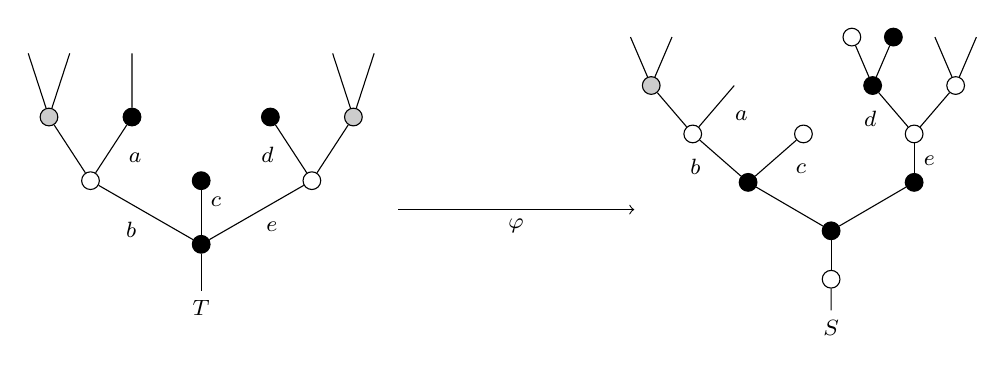
\begin{tikzpicture}[grow=up,auto,level distance=2.3em,
every node/.style = {font=\footnotesize},
dummy/.style={circle,draw,inner sep=0pt,minimum size=2.25mm}]
	\tikzstyle{level 2}=[sibling distance = 4em]
	\tikzstyle{level 3}=[sibling distance = 3em]
	\tikzstyle{level 4}=[sibling distance = 1.5em]
	\node at (0,0.25) {$T$}
		child{node [dummy,fill = black] {}
			child{node [dummy,fill=white] {}
				child{node [dummy,fill = black!20] {}
					child
					child
				}
				child{node [dummy,fill = black] {}
				edge from parent node [near end] {$d$}}
			edge from parent node [swap] {$e$}}
			child{node [dummy,fill=black] {}
			edge from parent node [swap, near end] {$c$}}
			child{node [dummy,fill=white] {}
				child{node [dummy,fill = black] {}
					child
				edge from parent node [swap, near end] {$a\phantom{d}$}}
				child{node [dummy,fill = black!20] {}
					child
					child
				}
			edge from parent node {$b$}}
		};
\begin{scope}[level distance=1.75em]
	\tikzstyle{level 3}=[sibling distance = 6em]
	\tikzstyle{level 4}=[sibling distance = 4em]
	\tikzstyle{level 5}=[sibling distance = 3em]
	\tikzstyle{level 6}=[sibling distance = 1.5em]
	\tikzstyle{level 7}=[sibling distance = 0.75em]
	\node at (8,0) {$S$}
		child{node [dummy,fill = white] {}
			child{node [dummy,fill = black] {}
				child{node [dummy,fill = black] {}
					child{node [dummy,fill=white] {}
						child{node [dummy,fill = white] {}
							child
							child
						}
						child{node [dummy,fill = black] {}
							child{node [dummy,fill=black] {}
						}
							child{node [dummy,fill=white] {}}
						edge from parent node [near end] {$d$}}
					edge from parent node [swap] {$e\phantom{1}$}}
				}
				child{node [dummy,fill = black] {}
					child{node [dummy,fill=white] {}
					edge from parent node [swap, near end] {$c\phantom{1}$}}
					child{node [dummy,fill=white] {}
						child{
						edge from parent node [swap,near end] {$a\phantom{d}$}}
						child{node [dummy,fill = black!20] {}
							child
							child
						}
					edge from parent node [near end] {$\phantom{1}b$}}
				}
			}
		};
\end{scope}
	\draw [->] (2.5,1.5) -- node [swap] {$\varphi$} (5.5,1.5);
\end{tikzpicture}
\end{equation}
\end{example}


\begin{proposition}
One has an identification
\[
\Omega_G^e \simeq 
|\Omega_{G}^{\{+\infty\}_{\langle \bullet \rangle}}|.
\]
\end{proposition}


\begin{proof}
We note first that $\Omega_{G}^e$ contains all label maps that are $\{A,B\}$-inert. In fact, any map of $\Omega_{G}^e$ clearly has a unique factorization as such a label map followed by an underlying planar isomorphism of trees that replaces some of the $X$ and $B$ labels with $A$ labels.
We will refer to the former as label maps and to the latter as relabel maps.

We recall that 
$\Omega_{G}^{\{+\infty\}_{\langle n \rangle}}$
consists of trees with $2n+3$ types of labels: 
$X$-labels, $B$-labels and $2n+1$ distinct types of $A$-labels.
One can equivalently encode such a tree as a string 
$T_0 \to \cdots \to T_n$
of relabel maps. Indeed, the $A$-label nodes of $T_n$ in such a string are partitioned into $2n+1$ types according to that node's labels one the $T_i$ (which are either all $A$'s, some $X$'s and then $A$'s or some $B$'s and then $A$'s).
Moreover, a diagram
\[
\begin{tikzcd}
	T_0 \ar{r} \ar{d}[swap]{f_0} & 
	T_1 \ar{r} \ar{d}[swap]{f_1} & 
	\cdots \ar{r} &
	T_n \ar{d}[swap]{f_n} &
\\
	T'_0 \ar{r} &
	T'_1 \ar{r} &
	\cdots \ar{r} &
	T'_n 
\end{tikzcd}
\]
with $f_i$ label maps of $\Omega^{e}_G$ is then equivalent to a label map $f_n \colon T_n \to T'_n$ respecting all $2n+3$ labels 
in $\Omega_{G}^{\{+\infty\}_{\langle n \rangle}}$.
Since the string description above is also compatible with the simplicial structure maps in the obvious way, 
the result is now clear. 
\end{proof}


Our next task will be that of identifying a convenient Lan-final subcategory $\bar{\Omega}_G^{e} \hookrightarrow \Omega_G^e$.
We first introduce the auxiliary notion of alternating trees.
We recall the notion of input path (Notation \ref{INPUTPATH NOT})
$I(e) = \{f \in T \colon e \leq_d f\}$ for an edge $e \in T$, which naturally extends to $T$ in any of $\in \Omega, \Phi, \Omega_G, \Phi_G$.

\begin{definition}\
A $G$-tree $T \in \Omega_G$ is called \textit{alternating} if, for all leafs $l \in T$ one has that the input path $I(l)$ has an even number of elements.

Further, a vertex $e^{\uparrow} \leq e$ is called \textit{active}
if $|I(e)|$ is odd and \textit{inert} otherwise.

Finally, a tall map $T \xrightarrow{\varphi} T'$ between alternating $G$-trees is called a 
\textit{tall alternating map}
if for any inert vertex $e^{\uparrow} \leq e$ of $T$ one has that 
$T'_{ e^{\uparrow} \leq e)}$ is an inert vertex of $T'$.

We will denote the category of alternating $G$-trees and tall alternating maps by $\Omega_G^a$.
\end{definition}


\begin{example}
Two alternating trees (for $G=\**$ the trivial group) and a planar tall alternating map between them follow, with active nodes in black ($\bullet$) and white nodes in white ($\circ$).
\begin{equation}\label{REGALTERNMAP EQ}
\begin{tikzpicture}[grow=up,auto,level distance=2.3em,every node/.style = {font=\footnotesize},dummy/.style={circle,draw,inner sep=0pt,minimum size=1.75mm}]
	\tikzstyle{level 2}=[sibling distance = 4em]
	\tikzstyle{level 3}=[sibling distance = 3em]
	\tikzstyle{level 4}=[sibling distance = 1.5em]
	\node at (0,0.85) {$T$}
		child{node [dummy,fill = black] {}
			child{node [dummy,fill=white] {}
				child{node [dummy,fill = black] {}
					child
					child
				}
				child{node [dummy,fill = black] {}
				edge from parent node [near end] {$d$}}
			edge from parent node [swap] {$e$}}
			child{node [dummy,fill=white] {}
			edge from parent node [swap, near end] {$c$}}
			child{node [dummy,fill=white] {}
				child{node [dummy,fill = black] {}
					child
				edge from parent node [swap, near end] {$a\phantom{d}$}}
				child{node [dummy,fill = black] {}
					child
					child
				}
			edge from parent node {$b$}}
		};
\begin{scope}[level distance=1.75em]
	\tikzstyle{level 3}=[sibling distance = 6em]
	\tikzstyle{level 4}=[sibling distance = 4em]
	\tikzstyle{level 5}=[sibling distance = 3em]
	\tikzstyle{level 6}=[sibling distance = 1.5em]
	\tikzstyle{level 7}=[sibling distance = 0.75em]
	\node at (9,0) {$S$}
		child{node [dummy,fill = black] {}
			child{node [dummy,fill = white] {}
				child{node [dummy,fill = black] {}
					child{node [dummy,fill=white] {}
						child{node [dummy,fill = black] {}
							child
							child
						}
						child{node [dummy,fill = black] {}
							child{node [dummy,fill=white] {}
								child{node [dummy,fill = black] {}}
								child{node [dummy,fill = black] {}}
						}
							child{node [dummy,fill=white] {}}
						edge from parent node [near end] {$d$}}
					edge from parent node [swap] {$e\phantom{1}$}}
				}
				child{node [dummy,fill = black] {}
					child{node [dummy,fill=white] {}
					edge from parent node [swap, near end] {$c\phantom{1}$}}
					child{node [dummy,fill=white] {}
						child{node [dummy,fill = black] {}
							child{node [dummy,fill=white] {}
								child{node [dummy,fill = black] {}
									child
								}
							}
						edge from parent node [swap,near end] {$a\phantom{d}$}}
						child{node [dummy,fill = black] {}
							child
							child
						}
					edge from parent node [near end] {$\phantom{1}b$}}
				}
			}
		};
\end{scope}
	\draw [->] (3,2) -- node [swap] {$\varphi$} (6,2);
\end{tikzpicture}
\end{equation}
The term ``alternating'' comes from the fact that no adjacent nodes have the same color. We note, however, that there is additional restriction: the ``outer'' vertices, i.e. those immediately below a leaf or the one immediately above the root, are necessarily black/active
(not, however, that this does \textit{not} apply to stumps).
%As for the map $\varphi$, we assume additionally that it is a planar map (so that by the tallness condition the root is sent to the root and leaves are sent to leaves while respecting the planar order) and that it sends the labelled edges of $T$ to the eponymous edges of $S$ (though this information is in fact redundant: only one such planar tall alternating map exists).
\end{example}

\begin{remark}
	One can extend Definition \ref{SUBSTITUTIONDATUM} to the alternating context by defining a substitution datum to be alternating if it is given by isomorphisms for inert nodes and by alternating maps for active nodes. It is then straightforward to check that Proposition \ref{SUBDATAUNDERPLAN PROP} and its equivariant analogue Proposition \ref{SUBDATAUNDERPLANG PROP} extend to give alternating analogues.
\end{remark}

\begin{definition}
	$\bar{\Omega}_G^e \hookrightarrow \Omega_G^e$ is the full subcategory of $(B,A,X)$-labeled trees whose underlying trees is alternating, active nodes are labeled by $X$, and passive nodes are labeled by $A$ or $B$. 
\end{definition}

We note that conditions (i) and (ii) in Definition \ref{EXTTREECAT DEF} imply that maps in 
$\bar{\Omega}_G^e$ are underlying alternating maps.

The following establishes the required finality of $\bar{\Omega}_G^e$ in $\Omega_G^e$.

\begin{proposition}\label{LXP PROP}
	For each $U \in \Omega_G^e$ there exists a unique 
	$\mathsf{lr}_X (U) \in \bar{\Omega}_G^e$ together with a unique planar label map of $\Omega_G^e$
	\[\mathsf{lr}_X (U) \to U.\]
	Furthermore, $\mathsf{lr}_X$ extends to a right retraction $\mathsf{lr}_X \colon \Omega_G^e \to \bar{\Omega}_G^e$.
\end{proposition}

\begin{proof}
	Given $U$, we form a collection of outer faces
	$\{U_i^A\} \amalg \{U_j^B\} \amalg \{U_k^X\}$
where the $U_i^A, U_j^b$ are simply the $A,B$-labeled nodes
and the $\{U_k^X\}$ are the maximal outer subtrees whose nodes have only $X$-labels (we note that these may possible be sticks). 
Lemma \ref{OUTERFACEUNION LEM} then guarantees that the $V_G(U_k^{X})$ are disjoint, so that one can apply (the equivariant version of Proposition \ref{BUILDABLE PROP})
to build 
\begin{equation}\label{LRXDEF EQ}
T = \mathsf{lr}(U) \to U
\end{equation}
such that $\{U_{v_{G e}}\} = \{U_i^A\} \amalg \{U_j^B\} \amalg \{U_k^X\}$. $T$ has an obvious $(B,A,X)$-labeling making 
(\ref{LRXDEF EQ}) into a label map, but we must still check $T \in \bar{\Omega}^{e}_G$, i.e. that $T$ is alternating with the $X$-labeled vertices being precisely the $X$-labeled vertices.
Let us now write any input path of $T$ as 
$I(e) = (e = e_n \leq e_{n-1} \leq \cdots \leq e_1 \leq e_0)$.
By Lemma \ref{OUTERFACEUNION LEM} and maximality of the $U_k^X$, no pair of consecutive vertices $v_{Ge_i}$ and $v_{Ge_{i+1}}$ can be both $X$-labeled.
On the other hand, again by Lemma \ref{OUTERFACEUNION LEM} any edge of $U$ belongs to some $U^X_k$ and therefore:
\begin{inparaenum}
	\item[(i)] at least one of in each pair of consecutive vertices $v_{Ge_i}$ and $v_{Ge_{i+1}}$ is $X$-labeled;
	\item[(ii)] if $r \in T$ is a root, $v_{G r}$ is $X$-labeled;
	\item[(iii)] if $l \in T$ is a leaf $v_{G l_{n-1}}$ is $X$-labeled.
\end{inparaenum}
This suffices to conclude $T \in \bar{\Omega}_{G}^e$, and
uniqueness of $T$ is immediate from the uniqueness in Lemma \ref{OUTERFACEUNION LEM}. 


It remains to check that $\mathsf{lr}_X$ in fact defines a functor. We consider the following diagram.
\[
\begin{tikzcd}
	\mathsf{lr}_X(U) \ar{r} \ar[dashed]{d}[swap]{\mathsf{lr}_X(f)} & U \ar{d}{f}
\\
	\mathsf{lr}_X(V) \ar{r} & V
\end{tikzcd}
\]
When $f$ is a root pullback map, we define $\mathsf{lr}_X(f)$ to likewise be a root pullback map. When $f$ is a rooted tall map, writing $T=\mathsf{lr}_X(U)$ one has a map of rooted $T$-substitution data
$\{\mathsf{lr}_X(V_{v_{G_e}})\} \to \{V_{v_{G_e}}\}$,
which after converted to a tree map yields the desired map 
$\mathsf{lr}_X(f)$.
To check that $\mathsf{lr}_X$ respects composition of maps, 
the only non immediate case is that of a root pullback followed by a rooted map, in which case this follows from Remark \ref{PULLCOMP REM}.
\end{proof}


\begin{example}
The following illustrates the $\mathsf{lr}_X$ construction when applied to the map $\varphi$ in (\ref{REGALTERNMAP EQ}).
\begin{equation}
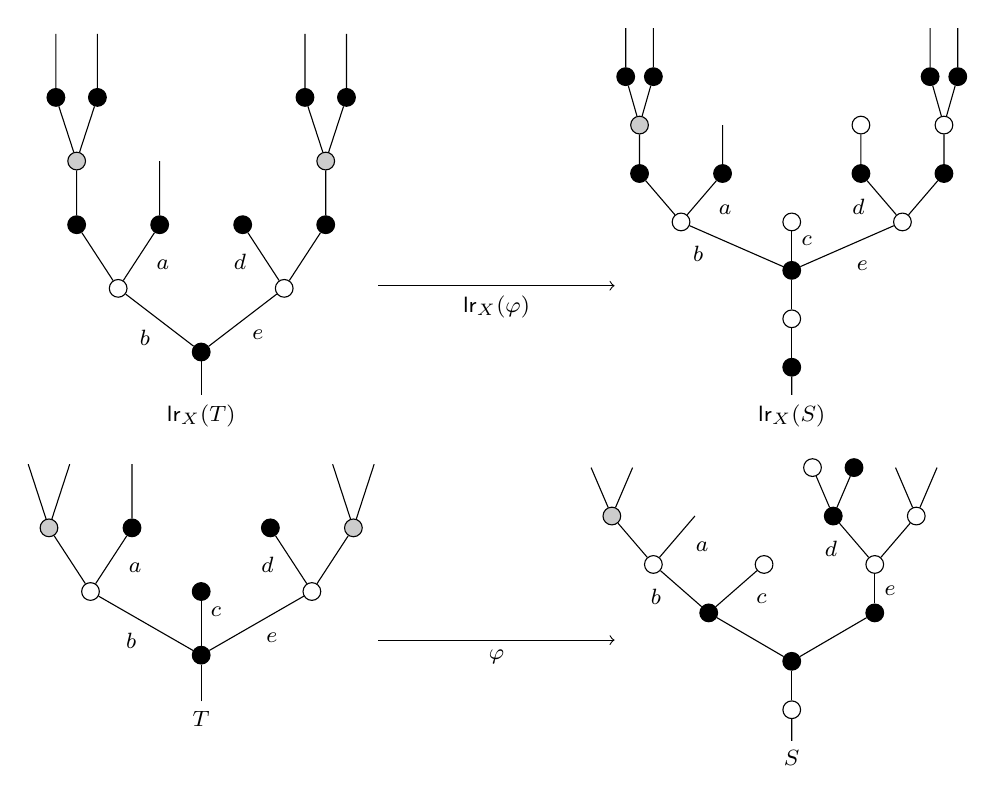
\begin{tikzpicture}[grow=up,auto,level distance=2.3em,
every node/.style = {font=\footnotesize},
dummy/.style={circle,draw,inner sep=0pt,minimum size=2.25mm}]
	\tikzstyle{level 2}=[sibling distance = 6em]
	\tikzstyle{level 3}=[sibling distance = 3em]
	\tikzstyle{level 4}=[sibling distance = 1.5em]
	\node at (0,0.85) {$\mathsf{lr}_X(T)$}
		child{node [dummy,fill = black] {}
			child{node [dummy,fill=white] {}
				child{node [dummy,fill = black] {}
					child{node [dummy,fill = black!20] {}
						child{node [dummy,fill = black] {}
							child}
						child{node [dummy,fill = black] {}
							child}
					}
				}
				child{node [dummy,fill = black] {}
				edge from parent node [near end] {$d$}}
			edge from parent node [swap] {$e$}}
			child{node [dummy,fill=white] {}
				child{node [dummy,fill = black] {}
					child
				edge from parent node [swap, near end] {$a\phantom{d}$}}
				child{node [dummy,fill = black] {}
					child{node [dummy,fill = black!20] {}
						child{node [dummy,fill = black] {}
							child}
						child{node [dummy,fill = black] {}
							child}
					}
				}
			edge from parent node {$b$}}
		};
\begin{scope}
	\tikzstyle{level 2}=[sibling distance = 4em]
	\tikzstyle{level 3}=[sibling distance = 3em]
	\tikzstyle{level 4}=[sibling distance = 1.5em]
	\node at (0,-3) {$T$}
		child{node [dummy,fill = black] {}
			child{node [dummy,fill=white] {}
				child{node [dummy,fill = black!20] {}
					child
					child
				}
				child{node [dummy,fill = black] {}
				edge from parent node [near end] {$d$}}
			edge from parent node [swap] {$e$}}
			child{node [dummy,fill=black] {}
			edge from parent node [swap, near end] {$c$}}
			child{node [dummy,fill=white] {}
				child{node [dummy,fill = black] {}
					child
				edge from parent node [swap, near end] {$a\phantom{d}$}}
				child{node [dummy,fill = black!20] {}
					child
					child
				}
			edge from parent node {$b$}}
		};
\end{scope}
\begin{scope}[level distance=1.75em]
	\tikzstyle{level 3}=[sibling distance = 6em]
	\tikzstyle{level 4}=[sibling distance = 4em]
	\tikzstyle{level 5}=[sibling distance = 3em]
	\tikzstyle{level 6}=[sibling distance = 1.5em]
	\tikzstyle{level 7}=[sibling distance = 1em]
	\node at (7.5,0.85) {$\mathsf{lr}_X(S)$}
		child{node [dummy,fill = black] {}
			child{node [dummy,fill = white] {}
				child{node [dummy,fill = black] {}
					child{node [dummy,fill=white] {}
						child{node [dummy,fill = black] {}
							child{node [dummy,fill = white] {}
								child{node [dummy,fill = black] {}
									child}
								child{node [dummy,fill = black] {}
									child}
							}
						}
						child{node [dummy,fill = black] {}
							child{node [dummy,fill=white] {}}
						edge from parent node [near end] {$d$}}
					edge from parent node [swap] {$e\phantom{1}$}}
					child{node [dummy,fill=white] {}
					edge from parent node [swap, near end] {$c\phantom{1}$}}
					child{node [dummy,fill=white] {}
						child{node [dummy,fill=black] {}
							child
						edge from parent node [swap,near end] {$a\phantom{d}$}}
						child{node [dummy,fill=black] {}
							child{node [dummy,fill = black!20] {}
								child{node [dummy,fill=black] {}
									child
								}
								child{node [dummy,fill=black] {}
									child
								}
							}
						}
					edge from parent node [near end] {$\phantom{1}b$}}
				}
			}
		};
\end{scope}
\begin{scope}[level distance=1.75em]
	\tikzstyle{level 3}=[sibling distance = 6em]
	\tikzstyle{level 4}=[sibling distance = 4em]
	\tikzstyle{level 5}=[sibling distance = 3em]
	\tikzstyle{level 6}=[sibling distance = 1.5em]
	\tikzstyle{level 7}=[sibling distance = 0.75em]
	\node at (7.5,-3.5) {$S$}
		child{node [dummy,fill = white] {}
			child{node [dummy,fill = black] {}
				child{node [dummy,fill = black] {}
					child{node [dummy,fill=white] {}
						child{node [dummy,fill = white] {}
							child
							child
						}
						child{node [dummy,fill = black] {}
							child{node [dummy,fill=black] {}
						}
							child{node [dummy,fill=white] {}}
						edge from parent node [near end] {$d$}}
					edge from parent node [swap] {$e\phantom{1}$}}
				}
				child{node [dummy,fill = black] {}
					child{node [dummy,fill=white] {}
					edge from parent node [swap, near end] {$c\phantom{1}$}}
					child{node [dummy,fill=white] {}
						child{
						edge from parent node [swap,near end] {$a\phantom{d}$}}
						child{node [dummy,fill = black!20] {}
							child
							child
						}
					edge from parent node [near end] {$\phantom{1}b$}}
				}
			}
		};
\end{scope}
	\draw [->] (2.25,2.5) -- node [swap] {$\mathsf{lr}_X(\varphi)$} (5.25,2.5);
	\draw [->] (2.25,-2) -- node [swap] {$\varphi$} (5.25,-2);
\end{tikzpicture}
\end{equation}
\end{example}




\newpage



\section{Filtration of cellular extensions}

Put together, the results in the previous section show that the free extension $\P[u]$ given by the pushout
\begin{equation}\label{CELLEXTPUSH EQ}
\begin{tikzcd}
  \mathbb F_G X \arrow[d, "u"'] \arrow[r] & \P \arrow[d]\\
  \mathbb F_G Y \arrow[r] & \P[u]
\end{tikzcd}
\end{equation}
is given by a left Kan extension along 
$(\bar{\Omega}_{G}^e)^{op} \xrightarrow{\mathsf{lr}} \Sigma_G^{op}$. So as to study the homotopical properties of the map $\P \to \P[u]$ we will identity a suitable filtration of this map, which will in turn be induced by a suitable filtration of the extension tree category $\bar{\Omega}_{G}^e$.


\subsection{Filtration pieces}

We now turn to the task of describing our filtration of $\bar{\Omega}_{G}^e$. 

Firstly, we write $V_X(T)$ (resp. $V_Y(T)$) to denote the set of (non-equivariant) vertices of $T$ with a $X$-label (resp. $Y$-label). 
We now define the \textit{degree} of $T \in \bar{\Omega}_{G}^e$,
denoted $|T|$, to be the sum $|T|_X + |T|_Y$, where $|T|_X$, $|T|_Y$ are defined by
\[
|T|_X = \dfrac{|V_X(T)|}{|G r|} = \sum\limits_{G v\in V_{G,X}(T)}\dfrac{|G v|}{|G r|},
\qquad
|T|_Y = \dfrac{|V_Y(T)|}{|G r|} = \sum\limits_{G v\in V_{G,Y}(T)}\dfrac{|G v|}{|G r|}
\]
for $G r$ the root orbit of $T$. 

Intuitively, $|T|_X$ counts the number of $X$-labeled vertices in each individual tree component of $T$.


\begin{remark}
	One of the key properties of the degrees just defined is that they are invariant under root pullback.
\end{remark}


\begin{definition}\label{TREE_FILTRATION_PIECES_DEFINITION}
We define subcategories of $\bar{\Omega}_{G}^e$:
  \begin{itemize}
  \item $\bar{\Omega}_G^e[\leq k]$ (resp. $\Omega_G^e[k]$) is the full subcategory of trees 
  $T \in \bar{\Omega}_G^e$ with $|T|\leq k$ (resp. $|T| = k$);
  \item $\bar{\Omega}_G^e[\leq k,-]$ (resp. $\bar{\Omega}_G^e[k,-]$) is the full subcategory of $\bar{\Omega}_G^e[\leq k]$ (resp. $\bar{\Omega}_G^e[k]$) of trees $T$ with $|T|_{Y}\neq k$;
  \item $\bar{\Omega}_G^e[k,0]$ is the full subcategory of 
  $\bar{\Omega}_G^e[k]$ of trees $T$ with $|T|_X = 0$ (or, equivalently, $|T|_{Y} = k$).
%  \item If $\Xi$ is any of the above categories, and $C\in \Sigma_G$, let $\Xi(C)$ denote the full subcategory of $\Xi$ spanned by those trees $T$ with $val(T) \simeq C$.
  \end{itemize}
The above definitions still hold if we replace $\bar\Omega_G^e$ with $\Omega_G^a$; in particular, we have vertical forgetful functors
\[
\begin{tikzcd}
  \bar\Omega_G^e[k,-] \arrow[dr, "\mathsf{fgt}"'] \arrow[rr, hookrightarrow] && \bar\Omega_G^e[k] \arrow[dl, "\mathsf{fgt}"]\\
  & \Omega_G^a[k]
\end{tikzcd}
\]
\end{definition}


\begin{remark}\label{LIMMOR REM}
  The categories $\bar{\Omega}_G^e[k]$ and $\bar{\Omega}_G^e[k,-]$ have only rather limited morphisms.
  In fact, all maps in these categories must be underlying quotients of trees. Indeed, it is clear from Definition \ref{EXTTREECAT DEF} that maps never lower degree and, moreover, degree is preserved iff $\mathcal{P}$-vertices are substituted by $\mathcal{P}$-vertices (rather than larger trees in $\bar{\Omega}_G^e$, which would necessarily possess $X$-vertices).
  
  Moreover, we have a clear isomorphism of categories $\bar\Omega_G^e[k,0] \simeq \Omega_G^a[k]$. 
\end{remark}


\begin{lemma}\label{MINUS_LAN_FINAL_LEMMA}
  $\bar{\Omega}_G^e[\leq k-1]$ is $\mathsf{Ran}$-initial in $\bar{\Omega}_G^{e}[\leq k,-]$ over $\Sigma_G$.
\end{lemma}

In the proof we will make use of the following construction on 
$\Omega_{G,e}$: given $T \in \Omega_{G,e}$ we will let $T_{\mathcal{P}}$ denote the result of replacing all $X$-labeled nodes of $T$ with $\mathcal{P}$-labeled nodes.

\begin{remark}\label{YINERT REM}
  Unlike the $\mathsf{lr}_{\mathcal{P}}$ construction of Proposition \ref{LXP PROP}, which defines a functor 
  $\mathsf{lr}_{\mathcal{P}} \colon
  \Omega_G^e \to \bar{\Omega}_G^e $,
  the construction 
  $(\minus)_{\mathcal{P}}$ does not define a full functor
  $\Omega_G^e \to \Omega_G^e$, instead being functorial, and the obvious maps $T_{\mathcal{P}} \to T$ natural, only with respect to the $Y$-inert maps of $\Omega_G^e$.
\end{remark}


\begin{example}
%  We observe that this construction is symmetric across all tree components, and hence, to give an example, it suffices to show want happens on a single component (i.e. when $G = \set{e}$).
Combining the $(\minus)_{\mathcal{P}}$ and $\mathsf{lr}_{\mathcal{P}}$ constructions one obtains a construction sending trees in $\bar{\Omega}^e_G$ to trees in $\bar{\Omega}^e_G$.
We illustrate this for the tree $T \in \bar{\Omega}^e_G$ below, where black nodes are $\P$-labeled, white nodes filled with $\times$ are $X$-labeled, and empty white nodes are $Y$-labeled.
\[
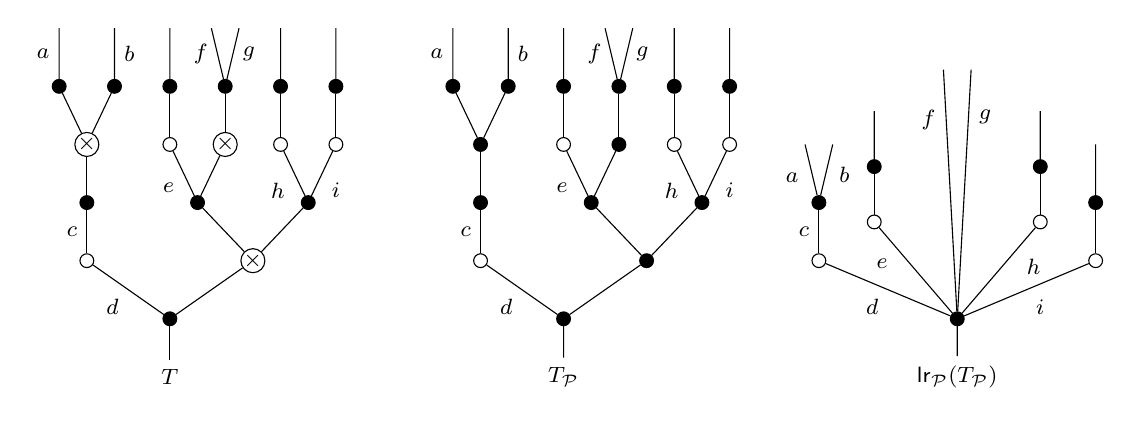
\begin{tikzpicture}
  [grow=up,auto,level distance=2.1em,every node/.style = {font=\footnotesize},dummy/.style={circle,draw,inner sep=0pt,minimum size=1.75mm}]
%  [grow=up, level distance = .8cm, auto, every node/.style={font=\small}, dummy/.style={circle,draw,inner sep=0.4mm, minimum size=2.25}]
    \tikzstyle{level 2}=[sibling distance=6em]
    \tikzstyle{level 3}=[sibling distance=4em]
    \tikzstyle{level 4}=[sibling distance=2em]
    \tikzstyle{level 5}=[sibling distance=2em]
    \tikzstyle{level 6}=[sibling distance=1em]
  \node{$T$}
  child{node [dummy, fill=black] {}%
    child{node [dummy] {$\times$}%
      child{node [dummy,fill=black] {}%
        child{node [dummy] {}%{\tiny y}%
          child{node [dummy, fill=black] {}%
            child{}
          }
          edge from parent node [swap] {$i$}
        }
        child{node [dummy] {}%{\tiny y}%
          child{node [dummy, fill=black] {}%
            child{}
          }
          edge from parent node {$h$}
        }
      }
      child{node [dummy, fill=black] {}%
        child{node [dummy] {$\times$}%
          child{node [dummy, fill=black] {}%
            child{edge from parent node [right]{$g$}} 
            child{edge from parent node [left]{$f$}} 
          }
        }
        child{node [dummy] {}%{\tiny y}%
          child{node [dummy, fill=black] {}%
            child{}
          }
          edge from parent node {$e$}
        }
      }
    }
    child{node [dummy] {}%{\tiny y}%
      child{node [dummy, fill=black] {}%
        child{node [dummy] {$\times$}%{\tiny $x$}%
          child{node [dummy, fill=black] {}%
            child{edge from parent node [swap] {$b$}}
          }
          child{node [dummy, fill=black] {}%
            child{edge from parent node {$a$}}
          }
        }
        edge from parent node {$c$}
      }
      edge from parent node {$d$}
    }
  };
  \node at (5,0){$T_{\mathcal{P}}$}
  child{node [dummy, fill=black] {}%
    child{node [dummy, fill=black] {}%
      child{node [dummy,fill=black] {}%
        child{node [dummy] {}%{\tiny y}%
          child{node [dummy, fill=black] {}%
            child{}
          }
          edge from parent node [swap] {$i$}
        }
        child{node [dummy] {}%{\tiny y}%
          child{node [dummy, fill=black] {}%
            child{}
          }
          edge from parent node {$h$}
        }
      }
      child{node [dummy, fill=black] {}%
        child{node [dummy, fill=black] {}%
          child{node [dummy, fill=black] {}%
            child{edge from parent node [right]{$g$}} 
            child{edge from parent node [left]{$f$}} 
          }
        }
        child{node [dummy] {}%{\tiny y}%
          child{node [dummy, fill=black] {}%
            child{}
          }
          edge from parent node {$e$}
        }
      }
    }
    child{node [dummy] {}%{\tiny y}%
      child{node [dummy, fill=black] {}%
        child{node [dummy, fill=black] {}%
          child{node [dummy, fill=black] {}%
            child{edge from parent node [swap] {$b$}}
          }
          child{node [dummy, fill=black] {}%
            child{edge from parent node {$a$}}
          }
        }
        edge from parent node {$c$}
      }
      edge from parent node {$d$}
    }
  };
  \tikzstyle{level 2}=[sibling distance=2em]
  \tikzstyle{level 4}=[sibling distance=1em]
  \node at (10,0){$\mathsf{lr}_{\mathcal{P}}(T_{\mathcal{P}})$}
  child{node [dummy,fill=black] {}%
    child{node [dummy] {}%{\tiny y}%
      child{node [dummy, fill=black] {}%
        child{}
      }
      edge from parent node [swap]{$i$}
    }
    child[level distance = 3.5em]{node [dummy] {}%{\tiny y}%
      child[level distance = 2em]{node [dummy, fill=black] {}%
        child{}
      }
      edge from parent node [swap,near end] {$h$}
    }
    child[sibling distance=1em, level distance = 9em]{edge from parent node [swap, very near end]{$g$}}
    child[sibling distance=1em, level distance = 9em]{edge from parent node [very near end]{$f$}}
    child[level distance = 3.5em]{node [dummy] {}%{\tiny y}%
      child[level distance = 2em]{node [dummy, fill=black] {}%
        child{}
      }
      edge from parent node [near end]{$e$}
    }
    child{node [dummy] {}%{\tiny y}%
      child{node [dummy, fill=black] {}%
        child{edge from parent node [swap,near end]{$b$}}
        child{edge from parent node [near end] {$\phantom{b}a$}}
        edge from parent node {$c$}
      }
      edge from parent node {$d$}
    }
  };    
\end{tikzpicture}
\]
\end{example} 


\begin{proof}[Proof of Lemma \ref{MINUS_LAN_FINAL_LEMMA}]
Just as in the proof of Lemma \ref{LANPULLCOMA LEM}, for each 
$C \in \Sigma_G$, 
the under categories
$C \downarrow \bar{\Omega}_G^e[\leq k-1]$,
$C \downarrow \bar{\Omega}_G^e[\leq k,-]$
have initial subcategories 
$C \downarrow_{\mathsf{r},\simeq} \bar{\Omega}_G^e[\leq k-1]$.
$C \downarrow_{\mathsf{r},\simeq} \bar{\Omega}_G^e[\leq k,-]$
of those objects
$(S,q \colon C \to \mathsf{lr}(S))$ such that 
$q$ is an ordered isomorphism on roots,
and thus an isomorphism in $\Sigma_G$.

It now suffices to show (cf. (\cite[X.3.1]{McL})) that for each
$(S,q \colon C \to \mathsf{lr}(S))$ in 
$C \downarrow_{\mathsf{r},\simeq} \bar{\Omega}_G^e[\leq k,-]$
the undercategory
\begin{equation}\label{UNDERCATPR EQ}
	(S,q) \downarrow  
	(C \downarrow_{\mathsf{r},\simeq} \bar{\Omega}_G^e[\leq k-1])
\end{equation}
is non-empty and connected. 
Moreover, we note that an object in 
(\ref{UNDERCATPR EQ})
is uniquely encoded by a map $T \to S$ inducing a rooted isomorphism on $\mathsf{lr}$.

The case $S\in \Omega_G^e[\leq k-1]$ is immediate. 
Otherwise, since $|S|_Y \neq k$ it is
$|\mathsf{lr}_{\mathcal{P}}(S_{\mathcal{P}})|<k$
and the map 
$\mathsf{lr}_{\mathcal{P}}(S_{\mathcal{P}}) \to S$,
which is a rooted isomorphism on $\mathsf{lr}$, shows that
(\ref{UNDERCATPR EQ}) is indeed non-empty.

  
Otherwise, given any rooted tall map $T \to S$ with 
$T \in \bar{\Omega}_G^e[k-1]$ (which gives a rooted isomorphism on $\mathsf{lr}$ and thus encodes a unique object of (\ref{UNDERCATPR EQ})). One can then form a diagram
\begin{equation}\label{K-1LANFINAL EQ}
\begin{tikzcd}
	      & S & \mathsf{lr}_{\mathcal{P}}(S_{\mathcal{P}}) \ar{l}
\\
	T \ar{ur} \ar{r} & T' \ar{u}[swap]{Y-\text{inert}} & \mathsf{lr}_{\mathcal{P}}(T'_{\mathcal{P}}) \ar{l} \ar{u}
\end{tikzcd}
\end{equation}
where $T \to T' \to S$ is the natural factorization such that the second map is $Y$-inert, i.e., $T'$ is obtained from $T$ by simply relabeling to $X$ those $Y$-labeled vertices of $T$ that become $X$-vertices in $S$. Note that the existence of the right square in (\ref{K-1LANFINAL EQ}) follows from the map $T' \to S$ being $Y$-inert together with Remark \ref{YINERT REM}.
Since (\ref{K-1LANFINAL EQ}) becomes a diagram of rooted  isomorphism on $\mathsf{lr}$, if produces the necessary zigzag connecting the objects $T \to S$ and 
$\mathsf{lr}_{\mathcal{P}}(S_{\mathcal{P}}) \to S$
in (\ref{UNDERCATPR EQ}), finishing the proof.
%
%
%Further, given any other element
%\begin{equation}
%    \label{K-1_LAN_FINAL_EQ2}
%    \begin{tikzcd}
%      val(S) && val(T) \arrow[ll, "f"']\\
%      & C \arrow{ur}[swap]{q_S} \arrow[ul, "q_T"]
%    \end{tikzcd}
%  \end{equation}
%  in the overcategory, consider the following zig-zag of maps connecting the objects (\ref{K-1_LAN_FINAL_EQ1}) and (\ref{K-1_LAN_FINAL_EQ2}):
%\begin{equation}\label{K-1_LAN_FINAL_DIAGRAM}
%\begin{tikzcd}
%	&& S &&
%\\[20pt]
%	&& \tilde q_T^*(S) \arrow[u, "\tilde q_T"'] &&
%\\
%	S^\wedge_\P \arrow[uurr, "\partial_\P"] &
%	\tilde q_T^*(S^\wedge_\P) \arrow[l, "\tilde q_T"'] \arrow[ur, "\partial_\P"] \arrow[rr, "\partial_\P"] &&
%	 T' \arrow[ul, "\partial_\P"'] & T \arrow[l, "\partial_Y"'] \arrow[uull, "f"']
%\\[20pt]
%	&& C \arrow[ull, "q_S"] \arrow[ul, "q_T"'] \arrow[ur, "q_T"] \arrow[urr, "q_T"'] 
%\end{tikzcd}
%\end{equation}
%  Here, we have omitted the notation ``$val$'' from the top three rows. To understand this diagram, we first record that we have a factorization:
%  \[
%  q_S = \tilde q_T q_T,
%  \]
%  Then, if we let $C_S = val(S) = val(S^\wedge_\P)$ and $C_T = val(T)$, we have
%  \[
%  C \xrightarrow{q_T} C_T \xrightarrow{\tilde q_T} C_S
%  \]
%  and hence, by the unique factorization of maps in $\Omega_{G,e}$, a factorization% via Remark \ref{OMEGA_E_REMARKS} (2), a factorization
%  \[
%  \begin{tikzcd}
%    C_T \arrow[d, "\tilde q_T"'] \arrow[r, dashed] & \tilde q_T^*(S^\wedge_\P) \arrow[d, dashed, "\tilde q_T"]\\
%    C_S \arrow[r] & S^\wedge_\P
%  \end{tikzcd}
%  \]
%  (where we are recording $C \to val(S)$ as a planar-tall map $C \to S$). 
%  A similar analysis shows that the top left trapezoid commutes. 
%
%  The other regions also commute by a straightforward analysis. Indeed, the top right trapezoid commutes by unique factorization, and finally the middle triangle of $\partial_\P$ maps commutes since $(\tilde q_T^*S)^\wedge_\P = \tilde q^*_T(S^\wedge_\P)$. 
%  
%  Lastly, we must check that the middle two maps are in fact elements of the appropriate overcategory. This follows from the fact that $S^\wedge_\P$ and $T$ have $|-|_Y < k$. Thus, the overcategory in question is connected, as desired.
\end{proof}


Similarly to the $(\minus)_{\mathcal{P}}$ construction,
there is also a construction $T_Y$ which replaces all $X$-labels of $T \in \Omega_G^e$ with $Y$-labels. Moreover, in this case the construction restricts directly to a construction on 
$\bar{\Omega}_G^e$,
which is easily seen to be functorial (and the $T_Y \to T$ maps natural) with regards to $\mathcal{P}$-inert maps. Remark \ref{LIMMOR REM} thus implies that 
$(\minus)_Y \colon \bar{\Omega}_G^e[k] \to 
\bar{\Omega}_G^e[k,0]$
is a left retraction, 
resulting in the following.
\begin{lemma}
  \label{ZERO_LAN_FINALITY_LEMMA}
  $\bar{\Omega}_G^{e}[k,0]$ is $\mathsf{Ran}$-initial in $\bar{\Omega}_G^e[k]$ over $\Sigma_G$.
\end{lemma}

%\begin{proof}[Proof of Lemma \ref{ZERO_LAN_FINALITY_LEMMA}]
%  This follows analogously to Lemma \ref{MINUS_LAN_FINAL_LEMMA}, by replacing Diagram \ref{K-1_LAN_FINAL_DIAGRAM} with the diagram below:
%  \[
%  \begin{tikzcd}
%    && S & \\[20pt]
%    &&\tilde q_T^*(S) \arrow[u, "\tilde q_T"]\\
%    S^\wedge_Y \arrow[uurr, "\partial_Y"] && \tilde q_T^*(S^\wedge_Y) \arrow[ll, "\tilde q_T"'] \arrow[u, "\partial_Y"] \arrow[rr, "\partial_Y"] && T \arrow[ull, "\partial_Y"'] \arrow[uull, "f"']\\
%    && C \arrow[ull, "q_S"] \arrow[u, "q_T"] \arrow[urr, "q_T"'] 
%  \end{tikzcd}
%  \]
%\end{proof}


In what follows we write $N^e \colon \Omega_G^{e,op} \to \mathcal{V}$ for the functor in (\ref{FREEEXTUSEFCOLNEW EQ}),
and abuse notation by likewise writing $N^e$ for any of its restrictions to the subcategories in 
Definition \ref{TREE_FILTRATION_PIECES_DEFINITION}.

We are now in a position to produce the desired filtration of the map $\mathcal{P} \to \mathcal{P}[u]$ in 
(\ref{CELLEXTPUSH EQ}).

\begin{definition}
  \label{PK_DEFN}
  Let $\P_k$ denote the left Kan extension
\[
\begin{tikzcd}
	|[alias=U]| \bar{\Omega}_G^e[\leq k]^{op} \arrow[r, "N^e"] \arrow[d, "\mathsf{lr}"'] & \V
\\
	\Sigma_G^{op} \arrow[ur, "\P_k"', ""{name=V}]
	\arrow[Rightarrow, from=U, to=V]
\end{tikzcd}
\]
\end{definition}
Noting that $\bar{\Omega}_G^e[\leq 0] \simeq \Sigma_G$ (since $|T|=0$ only if $T$ is a $G$-corolla with $\mathcal{P}$-labeled vertex) and that $\bar{\Omega}_G^e$
is the union of (the nerves of) the 
$\bar{\Omega}_G^e[\leq k]$, one has a filtration
\begin{equation}\label{FILT EQ}
	\mathcal{P} = 
	\mathcal{P}_0 \to 
	\mathcal{P}_1 \to
	\mathcal{P}_2 \to
	\cdots \to 
	\colim_k \mathcal{P}_k = \mathcal{P}[u].
\end{equation}


To analyze (\ref{FILT EQ}) homotopically we will further make use of a pushout description of each individual map 
$\mathcal{P}_{k-1} \to \mathcal{P}_k$. To do so, we note that the diagram of inclusions
\begin{equation}\label{INCDIAG EQ}
\begin{tikzcd}
	\bar{\Omega}_G^{e}[k,-] \arrow[d] \arrow[r] &
	\bar{\Omega}_G^{e}[\leq k,-] \arrow[d]
\\
	\bar{\Omega}_G^e[k] \arrow[r] &
	\bar{\Omega}_G^e[\leq k]
\end{tikzcd}
\end{equation}
is a pushout of at the level of nerves.
Indeed, this follows since
\[
\bar{\Omega}_G^e[k] \cap 
\bar{\Omega}_G^{e}[\leq k,-]
= \bar{\Omega}_G^{e}[k,-],
	\qquad
\bar{\Omega}_G^e[k] \cup 
\bar{\Omega}_G^{e}[\leq k,-]
= \bar{\Omega}_G^{e}[\leq k],
\]
and since a map $T \to S$ in 
$\bar{\Omega}_G^e[\leq k]$
will be in one of subcategories in (\ref{INCDIAG EQ}) iff $T$ is.

Since Lemma \ref{MINUS_LAN_FINAL_LEMMA} provides an identification 
$\Lan_{\bar{\Omega}_{G,e}[\leq k,-]^{op}}N^e \simeq
\Lan_{\bar{\Omega}_{G,e}[\leq k-1]^{op}}N^e = \mathcal{P}_{k-1}$,
applying left Kan extensions to (\ref{INCDIAG EQ}) yields the pushout diagram below.
\begin{equation}
  \label{FILTRATION_LAN_SQUARE_DIAGRAM}
  \begin{tikzcd}
    \Lan_{\bar{\Omega}_{G,e}[k,-]^{op}}N^e \arrow[d] \arrow[r] & \P_{k-1} \arrow[d]\\
    \Lan_{\bar{\Omega}_{G,e}[k]^{op}}N^e \arrow[r] & \P_k
  \end{tikzcd}
\end{equation}


{\color{red} HERE THERE}

%Finally, we show that each layer $\Omega_G^e[\leq k]$ can be built from $\Omega_{G}^e[\leq k-1]$ via a pushout which attaches trees with precise degree $k$. 
%While dealing with general pushouts of categories requires solving a ``word problem'' on morphisms, we will only work in cases where the problem collapses. We recall that, given a square of categories
%\[
%\begin{tikzcd}
%  \mathcal A \arrow[d] \arrow[r] & \mathcal C \arrow[d]\\
%  \mathcal C \arrow[r] & \mathcal D
%\end{tikzcd}
%\]
%if the nerve of this square is a pushout in $\sSet$, then this is a pushout of categories (since the nerve is the inclusion of a reflective subcategory).


%If we further assume that the span of functors is built out of fully-faithful inclusions, these pushouts behave as nicely as possible with left Kan extensions.
%\begin{lemma}
%  \label{LAN_PUSHOUT_LEMMA}
%  Given any diagram in categories of the form 
%\[
%\begin{tikzcd}
%  \mathcal A \arrow[d] \arrow[r, "f"] & \mathcal C \arrow[d, %"i"]\\
%  \mathcal B \arrow[r, "g"] & \mathcal D \arrow[r, "Y"] \arrow[d, "j"] & \V \\
%  & \mathcal D
%\end{tikzcd}
%\]
%such that the square is a nerve pushout of fully-faithful %functors, then $\Lan_j Y$ is the pushout of the induced span
%\[
%\begin{tikzcd}
%  \Lan_{j i f}(Y i f) \arrow[r] \arrow[d] & \Lan_{j i}(Y i)\\
%  \Lan_{j g}(Y g).
%\end{tikzcd}
%\]
%\end{lemma}
%\begin{proof}
%  By the universal property of left Kan extensions, it suffices to show that, for any functor $Z: \V \to \D$, the natural map
%  \[
%  \V^\D(Y, Z j) \longto \V^{\mathcal B} (Y g, Z j g) \prod\limits_{\V^{\mathcal A}(Y i f, Z j i f)} \V^{\mathcal C}(Y i, Z j i)
%  \]
%  is a bijection. These two sets give the same data: a collection of maps $\Phi_b: Y(b) \to Z(b)$ and $\Phi_c:Y(c) \to Z(c)$ for all $b\in \mathcal B$ and $c \in \mathcal C$, such that $\Phi_b = \Phi_c$ whenever $b = c \in \mathcal A$. In general, the compatibilites required on the right are less demanding. However, with the above assumptions, a map $d \to d'$ in $\mathcal D$ is \textit{uniquely} a map in $\mathcal A$, $\mathcal B \setminus \mathcal A$, or $\mathcal C \setminus \mathcal A$, and thus all the necessary compatibilities are covered by (at least) one of the $\set{\Phi_b}$ or $\set{\Phi_c}$. 
%\end{proof}




\subsection{Notation}
\todo[inline]{Luis: should this be stated earlier when defining the categorical wreath products?}

In order to state our filtration result, we will need to identify another categorical construction. This filtration will be built out of ``pushout products over trees of maps of sequences''. This subsection is dedicated to making that statement precise.

\begin{definition}
  Given a map $u: Y_0 \to Y_1$ of $G$-symmetric sequences $\V^{\Sigma_G^{op}}$, and $(A,D) \in \mathsf F \wr \Sigma_G$, we borrow notation from \cite{BM03} and define the functor
\[
[u]^D: (0 \to 1)^A \to \V
\]
as the composite
\[
(0 \to 1)^A \to \mathsf F \wr \V \xrightarrow{\times} \V
\]
where the first map is defined on $\xi: A \to \set{0,1}$ by
\[
(a \mapsto \xi(a)) \mapsto (A, (a \mapsto Y_{\xi(a)}(D(a))))
\]
\end{definition}

%We recall that, in a general category $\mathcal C$, a subcategory $\mathcal C' \subseteq \mathcal C$ is called \textit{convex} if whenever $c' \in \mathcal C'$ and $c \to c'$ is an arrow in $\mathcal C$< then both $c'$ and the map are in $\mathcal C'$. 

\begin{definition}
  \label{Q_DEFINITION}
  Given $u: Y_0 \to Y_1$ and $(A,D)\in \mathsf F \wr \Sigma_G$ as before, let $\mathsf{pc}(A)$ denote the 
%be a convex subcategory of $(0 \to 1)^A$. We define 
%\[
%Q_{\mathcal C}[u]^D := \colim_{\mathcal C}[u]^D.
%\]
%Moreover, given nested convex subcategories $\mathcal C' \subseteq \mathcal C$, we let
%\[
%[u]^D\square_{\mathcal C'}^{\mathcal C}: Q_{\mathcal C'}[u]^D \to Q_{\mathcal C}[u]^D
%\]
%denote the unique natural map.
%
%In particular, if $\mathcal C$ is the full 
``punctured cube'' subcategory 
\[
\mathsf{pc}(A) := (0 \to 1)^A \setminus \set{(1)_a} \subseteq (0 \to 1)^A,
\]
and define 
\[
Q[u]^D := \colim_{\mathsf{pc(A)}}[u]^D,
\]
and
\[
[u]^{\square D}: Q[u]^D \to \bigotimes\limits_{a \in A}Y_1(D(a))
\]
as the natural map.
\end{definition}

\subsection{Filtration Result}

We can now state our filtration of the cellular extension $\P \to \P[u]$. 

\begin{theorem}
  \label{FILTRATION_THEOREM}
  Let $\P$ be a genuine $G$-operad, and suppose we are given a map of $G$-symmetric sequences $u: Y_0 \to Y_1$. Then we have a filtration in $G$-sequences of the cellular extension
\[
\P = \P_0 \to \P_1 \to \ldots \to \colim(\P_i) = \P[u],
\]
where $\P_{k-1} \to \P_k$ is given by the pushout
\[
\begin{tikzcd}
  \Lan_{\bar\Omega_G^e[k,-]^{op}}N^e \arrow[d] \arrow[r] & \P_{k-1} \arrow[d]\\
  \Lan_{\bar\Omega_G^e[k]^{op}}N^e \arrow[r] & \P_k
\end{tikzcd}
\]
where each $\Lan$ is over the leaf-root functor associated to the given category.

Levelwise, for each $C\in \Sigma_G$, we have a filtration of $\P(C) \to \P[u](C)$ in $\V^{\mathrm{Aut}(C)}$, where $\P_{k-1}(C) \to \P_k(C)$ is given by the pushout
\[
\begin{tikzcd}
  \coprod\limits_{[T] \in \Omega_G^a[k](C)/\simeq} \left( \bigotimes\limits_{v \in V_{G,\P}(T)}\P(T_v) \otimes Q[u]^{\mathbb V_{G,in}(T)} \right) \otimes_{\mathrm{Aut}(T)} \mathrm{Aut}(C) \arrow[r] \arrow[d] & \P_{k-1}(C) \arrow[d] \\
   \coprod\limits_{[T] \in \Omega_G^a[k](C)/\simeq} \left( \bigotimes\limits_{v \in V_{G,\P}(T)}\P(T_v) \otimes \bigotimes\limits_{v \in V_{G,in}(T)} Y_1(T_v) \right) \otimes_{\mathrm{Aut}(T)} \mathrm{Aut}(C) \arrow[r] & \P_k(C)
\end{tikzcd}
\]
where the left vertical map is the iterated box product
\[
\coprod \mathop{\square}\limits_{V_{G,\P}(T)}\iota_{\P(T_v)}\mathop{\square} [u]^{\square \mathbb V_{G,in}(T)},
\]
$\iota_{\P(T_v)}$ is the canonical map $\varnothing \to \P(T_v)$ out of the initial object, and $\Omega_G^a[k](C)$ is as in Definnition \ref{TREE_FILTRATION_PIECES_DEFINITION}.
\end{theorem}

\begin{proof}
%  Combining Lemmas \ref{LAN_PUSHOUT_LEMMA} and \ref{TREE_CATS_DECOMP_LEMMA}, we have that $\P_k$ can be computed as the pushout
The first result is just a restatement of Diagram (\ref{FILTRATION_LAN_SQUARE_DIAGRAM}). Levelwise analysis follows from understanding the left-hand vertical map of Diagram (\ref{FILTRATION_LAN_SQUARE_DIAGRAM}), which we will denote 
\[
l[k]: L_1[k] \to L_2[k]. 
\]
By stacking left Kan extensions, we have
\[
%\Lan_{\bar\Omega_G^e[k]^{op}}N^e
L_i[k] \simeq \Lan_{\Omega_G^a[k]}(\Lan_{\bar\Omega_G^e[\epsilon_i] \to \Omega_G^a[k]}N^e),
\]
where $[\epsilon_1] = [k,-]$ and $[\epsilon_2] = [k]$. 
Evaluating at $C \in \Sigma_G$ using pointwise left Kan extensions yields
\[
L_i[k](C) \simeq \mathop{\colim}\limits_{\substack{\Omega_G^{a,op} \downarrow_{\mathsf r} C\\ T \xleftarrow{\simeq} C}}
\left( \mathop{\colim}\limits_{\substack{\bar\Omega_G^e[\epsilon_i]^{op} \downarrow_{\mathsf r} T \\ T^e \leftarrow T}}N^e(T^e)) \right).
\]
Further, we observe that $\bar\Omega_G^e[k]^{op} \downarrow_{\mathsf r} T$ is equivalent to the cube category $(0 \to 1)^{V_{G,in}(T)}$ (with only $\mathrm{Aut}(T)$-induced isomorphisms), while $\bar\Omega_G^e[k,-]^{op} \downarrow_{\mathsf  r} T$ is similarly equivalent to the punctured cube category $\mathsf{pc}(V_{G,in}(T))$.
Unpacked, these statements, in particular that cube categories have terminal objects, Lemma \ref{ZERO_LAN_FINALITY_LEMMA}, 
and the fact that $\Omega_G^{a,op}\downarrow_{\mathsf r}C$ is a groupoid, combine to imply that $l[k]$ is equivalent to the map
\[
\coprod\limits_{[T] \in \Omega_G^{a,op}[k](C)/\simeq} \left( \bigotimes\limits_{V_{G,\P}(T)} \P(T_{Gv}) \otimes Q[u]^{V_{G,in}(T)} \to N^e(T_Y) \right) \otimes_{\mathrm{Aut}(T)}\mathrm{Aut}(C),
\]
as desired.

% Repeating the above analysis for $L_1[k](C)$, we find
% \[
% L_1[k](C) \simeq \coprod\limits_{[T] \in \Omega_G^{a,op}[k](C)/\simeq} \left( \colim_{\mathsf{pc}(V(T))}Q[\bar u]^{N^e} \right) \otimes_{\mathrm{Aut}(T)}\mathrm{Aut}(C),
% \]
% where

% COME BACK HERE 

% By Lemma \ref{ZERO_LAN_FINALITY_LEMMA}, we may replace the bottom left corner with $\Lan_{\Omega_{G,e}[k,0]^{op}} N^e$.
% %$\colim_{\mathbb T_e^0[k]^{op}\downarrow n} N^e$. 
% Now, given $T\in \Omega_{G,e}[k,0]$, let $[T]$ denote the isomorphism class of $T$ in $\Omega_{G,e}[k,0]$. With this notation, the bottom left corner can further be identified with
% \[
% \displaystyle\coprod_{[T]\in \Omega_{G,e}[k,0](C)/\simeq}N^e(T)\otimes_{\mathrm{Aut}(T)}\Aut(C) 
% = \displaystyle\coprod_{[T]}
% \left(\bigotimes_{v\in V_{G,\P}(T)}\P(T_v) \otimes \bigotimes_{v\in V_{G,Y}(T)}Y_1(T_v) \right)
% \otimes_{\mathrm{Aut}(T)}\Aut(C).
% \]

% Next, we observe that the non-invertible morphisms of $\Omega_{G,e}[k,-]^{op}\downarrow C$ are just those which change the labeling of some nodes from $X$ to $Y$. Given $S$ and $T$ in $\Omega_{G,e}[k,-]$, write $S \sim T$ if they are in the same path component, and again note that this implies $|S| = |T|$, and moreover that $S$ and $T$ forget to the same $(\P;Z)$-alternating tree. Denote the path component of $T$ by $(T)$.

% We note that 
% %each connected component $(T)$ of $\mathbb T_e^-[k]$ is a generalized direct category (see \cite{nLabDirect}), and moreover 
% the set of path components of those trees with $val(T) = C$ is equal to the set of isomorphism classes in $\Omega_{G,e}[k,0](C)$, as both are just determined preicsely by their underlying $(\P;Z)$-alternating tree.

% To account for the $\Aut(C)$-action on the indexing category, we note that each connected component of $\Omega_{G,e}[k,-]^{op}\downarrow C$ has an action of $\mathrm{Aut}([T])$. Thus, the top left corner of Diagram (\ref{FILTRATION_LAN_SQUARE_DIAGRAM}) can be identified with the image of the colimit map below:
% \[
% \begin{tikzcd}
% \displaystyle\coprod_{[T]\in \Omega_{G,e}[k](C)/\sim}\left(\displaystyle\coprod_{S\in (T)\setminus{\set{T}}}N^e(S)\right) \otimes_{\mathrm{Aut}(T)}\Aut(C) \arrow[d, "\colim"]\\
% \displaystyle\coprod_{[T]}\left( \bigotimes_{v\in V_{G,\P}(T)} \P(T_v) \otimes Q[u]^{\mathbb V_{G,in}(T)}\right) \otimes_{\mathrm{Aut}(T)}\Aut(C)
% \end{tikzcd}
% \]
% where $Q[u]^{\mathbb V_{G,in}(T)}$ is the source of the pushout product map defined in Definition \ref{Q_DEFINITION}.

% Lastly, this left-side map is induced, via the naturality of Kan extesnions, by an inclusion of categories, in particular the product of multiple inclusions of categories, each corresponding the inclusion of a punctured cube into the full cube. Thus, after taking colimits, we have that the left-side map in Diagram (\ref{FILTRATION_LAN_SQUARE_DIAGRAM}) is in fact (multiple copies of) the pushout-product maps 
% \[
% [u]^{\Box \mathbb V_{G,in}(T)}: Q[u]^{\mathbb V_{G,in}(T)} \to \bigotimes_{v\in V_{G,in}(T)}Y_1(T_v)),
% \]
% as desired.
\end{proof}





\newpage

\section{Model Structures on Genuine Operads}
\todo[inline]{come back: this is all disorganized, internally, externally, everything}
\todo[inline]{replaced $\backslash$ F with $\mathcal F$ (as opposed to $\mathbb F$)}
\renewcommand{\F}{\ensuremath{\mathcal F}}


In order to encode the homotopical information inspired by $N_\infty$-operads dicussed in the introduction, we will introduce (semi) model structures on the categories $\V\Op_G$ and $\V\Op^G$ for a wide range of $\V$, which are true model categories in the cases we are most interested in (i.e. for $\V = \sSet$).  These model structures will be determined by a choice of weak indexing system, a generalization of the notion defined in \cite{BH15}. 


\subsection{Weak Indexing Systems}

We recall certain constructions found in \cite{Per17} relating graph subgroups, finite $H$-sets, and systems of categories.
\begin{definition}
  A \textit{$G$-graph subgroup} of $G\times \Sigma_n$ is a subgroup $\Lambda \leq G\times \Sigma_n$ such that $\Lambda \cap \Sigma_n = e$. Equivalently, $\Gamma = \Gamma(\phi)$ is the graph of some homomorphism $G \geq H \xrightarrow{\phi} \Sigma_n$. 
\end{definition}
\begin{definition}
  A \textit{$G$-vertex family} is a collection
\[
\F = \coprod\limits_{n\geq 0}\F_n
\]
where each $\F_n$ is a \textit{family} of $G$-graph subgroups of $G\times \Sigma_n$, closed under subgroups and conjugation. For a fixed $\F$, we call an $H$-set $A\in \mathsf F^H$ \textit{$\F$-admissible} if for some (equivalently, any) choice of bijection $A \leftrightarrow \set{1,\ldots, |A|}$, the graph subgroup of $G\times \Sigma_n$ encoding the induced $H$-action on $\set{1,\ldots, |A|}$ is in $\F_n$. 
\end{definition}
\begin{definition}
  For any $G$-vertex family $\F$, a $G$-tree $T\in \Omega_G$ is called \textit{$\F$-admissible} if, for each vertex $e_1\ldots e_n \leq e$ in $V(T)$, the set $\set{e_1,\ldots, e_n}$ is an $\F$-admissible $\Stab_G(e)$-set. We let $\Omega_\F\subseteq \Omega_G$ and $\Sigma_\F\subseteq \Sigma_G$ denote the full subcategories spanned by the $\F$-admissible trees.
\end{definition}
\begin{definition}
  A $G$-vertex family is called a \textit{weak indexing system} if $\Omega_\F$ is a \textit{sieve} of $\Omega_G$; that is, for any map $f:S \to T$ with $T\in \Omega_\F$, we have that $S$ (and the map $f$) are in $\Omega_\F$.
\end{definition}
We note that this always holds for any $\F$ is $f$ is an outer face or a quotient (for the latter, this follows from each $\F_n$ being closed under subgroups). However, closure under degeneracies implies that all trivial orbits $H/H$ are $\F$-admissible, while closure under inner faces implies that the $\F$-admissible sets are closed under  ``broad self-induction'': if $A \amalg H/K$ and $B$ are $\F$-admissible $H$- and $K$-sets, respectively, then $A \amalg H\times_K B$ is also an $\F$-admissible $H$-set. It also implies, in particular, the following:
\begin{lemma}
  \label{WEAK_INDEXING_VALENCE_LEMMA}
  The valence map $\mathsf{lr}$ restricts to a map $\mathsf{lr}: \Omega_\F \to \Sigma_\F$; that is, if $T$ is $\F$-admissible, so is $\mathsf{lr}(T)$. \qed
\end{lemma}


\begin{lemma}
  A weak indexing system $\F$ is an indexing system (in the sense of \cite{BH15}) if and only if all trivial $H$-sets are $\F$-admissible, for all $H\leq G$.
\end{lemma}
\begin{proof}
\todo[inline]{come back}
\end{proof}

We will define $\F$-model structures on $\V\Op_G$ for any weak indexing system $\F$; the $\F$-model structure on $\V\Sym_G$ will exist for any $G$-vertex family $\F$, but transfering requires the additional closure properties.


\subsection{Semi Model Structures on Genuine Operads}

Fix a $G$-vertex family $\F = \set{\F_n}$. For the following section, we fix the following about our base category $\V$:
\begin{definition}
  We say $\V$ satisfies \textsc{Assumption 1} (for $\F$) if the following hold:
  \begin{enumerate}
  \item $\V$ is a cofibrantly-generated Cartesian symmetric monoidal model category, and
  \item $\V$ is has cellular fixed point functors for all finite grouops %for each $T\in\Omega$, $\V^{G\times \Sigma_T}$ is $\F_T$-cellular 
(c.f. \cite{Stephan16}).
  \end{enumerate}
%where $\Sigma_T := \mathrm{Aut}(T)$, and $\F_T$ is the family of $G$-graph subgroups of $G\times \Sigma_T$ such that the induced action on $T$ defines an $\F$-admissible tree.
\end{definition}

\begin{definition}
  The \textit{$\F$-projective model structure} on $\V\Sym = \V^{\Sigma_G^{op}}$ is the unique model structure induced by the adjunction
\[
\V^{\Sigma_G^{op}} \leftrightarrows \V^{\Sigma_\F^{op}}.
\]
Explicitly, a map $f$ is a fibration (resp. weak equivalence) if $f(C)$ is one in $\V$ for all $C\in \Sigma_\F$.
\end{definition}

\begin{definition}
  A map $f: \O \to \P$ in $\V\Op_G$ is called a 
  \begin{enumerate}
  \item \textit{$\F$-fibration} (resp. $\F$-weak equivalence) if $f(C):\O(C) \to \P(C)$ is one in $\V$ for all $\F$-admissible $G$-corollas $C\in\Sigma_\F$.
  \item \textit{$\F$-cofibration} if it has the left lifting property against all maps which are both $\F$-fibrations and $\F$-weak equivalences.
  \item \textit{$\Sigma_\F$-cofibration} if $f$ is an $\F$-cofibration in $\V\Sym_G$.
  \end{enumerate}
\end{definition}
In particular, $\P\in \V\Op_G$ will be called \textit{$\F$-cofibrant} if $\varnothing \to \P$ is an $\F$-cofibration.
\begin{definition}
  The $\F$-model structure on $\V\Op_G$, if it exists, is the unique model structure with the above specified weak equivalences and fibrations. Equivalently, it is the transfered model structure along the adjoints
\[
\begin{tikzcd}
  \V\Op_G \arrow[r, shift right, "\mathsf{fgt}"'] & \V^{\Sigma_G^{op}} \arrow[l, shift right, "\mathbb F_G"'] \arrow[r, shift right] & \prod\limits_{\mathrm{Ob}(\Sigma_G)}\V \arrow[l, shift right] \arrow[r, shift right] & \prod\limits_{\mathrm{Ob}(\Sigma_\F)}\V \arrow[l, shift right]
\end{tikzcd}
\]
\end{definition}

Using general arguments of \cite{Hi03}, this structure would be cofibrantly generated, with generating arrows
\begin{align*}
  I_\F &= \sets{\mathbb F_G(\Sigma_G(-,C) \cdot i)}{C \in \Sigma_\F,\ i\in I}\\
  J_\F &= \sets{\mathbb F_G(\Sigma_G(-,C) \cdot j)}{C \in \Sigma_\F,\ j\in J},
\end{align*}
for $I$ (resp. $J$) the generating (trivial) cofibrations of $\V$.

\begin{definition}
  If $\F$ is the complete $G$-vertex family - so $\F_n$ is the family of \textbf{all} graph subgroups of $G\times \Sigma_n$ - we refer to the $\F$-model structure as the \textit{genuine} model structure.
\end{definition}

\begin{theorem}
  \label{GENUINE_SEMI_VOP_G_THM}
  The genuine semi-model structure on $\V\Op_G$ exists for all $\V$ satisfying \textsc{Assumption 1}.
\end{theorem}
\begin{proof}
    By general arguments of Kan \cite[11.6.1]{Hi03}, it suffices to show that any transfinite composite of cellular extensions $\P \to \P[u]$, each built by pushouts
\[
\begin{tikzcd}
  \mathbb F_G X \arrow[d, "u"'] \arrow[r] & \P \arrow[d]\\
  \mathbb F_G Y \arrow[r] & \P[u]
\end{tikzcd}
\]
where $u: X \to Y$ is a generating trivial cofibration and $\P$ is cofibrant in $\V^{\Sigma_G^{op}}_{gen}$, is itself a weak equivalence in $V^{\Sigma_G^{op}}_{gen}$. 

In particular, it suffices to show that, for $u$ a genuine level trivial cofibration and $\P$ genuine level cofibrant, any map $\P \to \P[u]$ is itself a genuine level trivial cofibration; since these are weaker conditions on $u$ and $\P$, and transfinite composition is levelwise, this implies the above result. This case follows from the levelwise filtration from Theorem \ref{FILTRATION_THEOREM}, by applying Propositions \ref{TREE_BOX_COFIBRANT_PROP} and \ref{FGTRIGHT PROP}.
\end{proof}

\begin{remark}
  In proving the above, we will often use the fact that, given families $\F \subseteq \bar \F$ of subgroups of a group $\Pi$, the identity map 
\[
\V^G_\F \to \V^G_{\bar \F}
\]
is left Quillen (and in particular preserves cofibrations). In particular, any $\F$-cofibration is a genuine cofibration.
\end{remark}

\begin{proposition}
  \label{TREE_BOX_COFIBRANT_PROP}
  Fix $T\in \Omega_G$, and suppose we are given cofibrations $f(Gv) \in \V^{\mathrm{Aut}(T_{Gv})}_{gen}$ for all $Gv\in V_G(T)$, such that $f(Gv) = f(\alpha(Gv))$ for all $\alpha\in \mathrm{Aut}(T)$. Then the iterated box product
\[
f^{\Box V_G(T)} = \mathop{\Box}\limits_{Gv \in V_G(T)} f(Gv)
\]
is a cofibration in $\V^{\mathrm{Aut}(T)}_{gen}$. 
\end{proposition}
\begin{proof}
  Using grafting composition $T \simeq C \circ (T^1_1, \ldots, T^{k_1}_1, T^1_2, \ldots, T^{k_r}_r)$, we go by induction on $|V_G(T)|$. The base cases of $|V_G(T)| = 0$ or 1 are trivial. Now, we note that we have a decomposition
\[
f^{\Box V_G(T)} = f(Gv_r) \Box \mathop{\Box}\limits_{i=1}^r\left( \left( f^{\Box V_G(T_i)} \right) ^{\Box k_i} \right)
\]
where $Gv_r$ is the root orbit. We will build this map in stages, preserving cofibrancy in each step.
\begin{itemize}
\item By induction, for each $i$, $f^{\Box V_G(T_i)}$ is a cofibration in $\V^{\mathrm{Aut}(T_i)}_{gen}$.
\item By Proposition \ref{POWERF PROP}, each $\left( f^{\Box V_G(T_i)} \right)^{\Box k_i}$ is a cofibration in $\V^{\Sigma_{k_i}\wr \mathrm{Aut}(T_i)}_{gen}$.
\item By Remark \ref{EXTERINTADJ EQ}, $\mathop{\Box}\limits_{i=1}^r\left(\left( f^{\Box V_G(T_i)} \right)^{\Box k_i}\right)$ is a cofibration in $\V^{\Pi \Sigma_{k_i} \wr \mathrm{Aut}(T_i)}_{gen}$.
\item By Proposition \ref{FGTLEFT PROP}, $f(Gv_r)$ is a cofibration in $\V^{\mathrm{Aut}(T)}_{gen}$.
\item Finally, by the decomposotion on $\mathrm{Aut}(T)$ and Proposition \ref{BIQUILLENG PROP}, we have the full $f^{\Box V_G(T)}$ is a cofibration in $\V^{\mathrm{Aut}(T)}_{gen}$, as desired.
\end{itemize}
If any $f(Gv)$ were trivial, then, during the appropriate step above, the resulting box product would again be trivial, by the same referenced results.
\end{proof}

\begin{corollary}
  For any $G$-vertex system $\F$, the $\F$-semi-model structure on $\V\Op_G$ exists.
\end{corollary}
\begin{proof}
  This follows from the proof of Theorem \ref{GENUINE_SEMI_VOP_G_THM}. In particular, it suffices to show that if $u: X\to Y$ is a level trivial $\F$-cofibration and $\P$ is level $\F$-cofibrant in $\V^{\Sigma_G^{op}}$, then the cellular extension $\P \to \P[u]$ is a level trivial $\F$-cofibration. However, such $u$ are level genuine cofibrations, and such $\P$ are level genuine cofibrant, and hence $\P \to \P[u]$ is a level trivial genuine cofibration, and hence a level trivial $\F$-cofibration.
\end{proof}

\subsection{True Model Structures}

\todo[inline]{come back}

\subsection{Preservation of Cofibrant Objects}

\todo[inline]{come back}

%%%%%%%%%%%%%% TRYING FOR V = SSET FIRST %%%%%%%%%%%%%%%%%%%%%%%%%

% We first prove the existence of these model structures when $\V = \sSet$. In this case, we denote $\V\Op_G$ by $\sOp_G$. 
% \begin{theorem}
%   The genuine model structure on $\sOp_G$ exists.
% \end{theorem}
% \begin{proof}
%   By general arguments of Kan \cite[11.6.1]{Hi03}, it suffices to show that any transfinite composite of cellular extension $\P \to \P[u]$, each built by pushouts
% \[
% \begin{tikzcd}
%   \mathbb F_G X \arrow[d, "u"'] \arrow[r] & \P \arrow[d]\\
%   \mathbb F_G Y \arrow[r] & \P[u]
% \end{tikzcd}
% \]
% where $u: X \to Y$ is a generating trivial cofibration in $\sSet^{\Sigma_G^{op}}_{gen}$, is itself a weak equivalence in $\sSet^{\Sigma_G^{op}}_{gen}$. 

% Since transfinite compositions are computed levelwise, it in fact suffices to show that each $\P \to \P[u]$ is a level trivial cofibration in $\sSet^{\Sigma_G^{op}}$; that is, that for all $C\in \Sigma_G$, $\P(C) \to \P[u](C)$ is a genuine trivial cofibration in $\sSet^{\mathrm{Aut}(C)}$. This is precisely the content of Lemma \ref{SSET_CELLULAR_LEVEL_COFIB_LEMMA}.
% \end{proof}

% \begin{theorem}
%   Cofibrant objects in $\sOp_G$ forget to cofibrant objects in $\sSet^{\Sigma_G^{op}}$. 
% \end{theorem}
% \begin{proof}
%   Similarly as above, it suffices to show that, for $u: X\to Y$ a cofibration in $\sSet^{\Sigma_G^{op}}$ and $\P$ underlyingly cofibrant in $\sSet^{\Sigma_G^{op}}$, the cellular extension $\P \to \P[u]$ is an underlying cofibration in $\sSet^{\Sigma_G^{op}}$. 
% \todo[inline]{come back}
% \end{proof}

% \begin{lemma}
%   \label{SSET_CELLULAR_LEVEL_COFIB_LEMMA}
%   If $u: X\to Y$ is a level trivial genuine cofibration in $\sSet^{\Sigma_G^{op}}$ (so $X(C) \to Y(C)$ is a genuine cofibration in $\sSet^{\mathrm{Aut}(C)}$), then $\P \to \P[u]$ is a level trivial genuine cofibration for any $\P \in \sOp_G$.
% \end{lemma}
% \begin{proof}
%   We first record that, since genuine cofibrations of simplicial sets are underlying, all $\P \in \sOp_G$ are levelwise genuine cofibrant, i.e. $\P(C)$ is cofibrant in $\sSet^{\mathrm{Aut}(C)}_{gen}$. 
% %  Usign the levelwise filtration
%   \todo[inline]{come back}
%   Follows from cofibration analysis.
% \end{proof}




%%%%%%%%%%%%%%%%%% LANS AND STUFF "RESULTS" %%%%%%%%%%%%%%%%%%

% Only transfer across the left-most adjunction requires proof. We will use the following result of White-Yau, following Fresse and Kan:
% \begin{theorem}
%   [{\cite[Theorem 2.2.2]{WY15}}]
%   \label{SEMI_MODEL_CATEGORY_EXISTENCE_THEOREM}
%   Suppose $\mathcal C$ is a cofibrantly generated model category, with generating (trivial) cofibrations $I$ (resp. $J$), and that we have a monadic adjunction $U: \mathsf{Alg}_{\mathbb F}(\mathcal C) \leftrightarrows \C: \mathbb F$ for some monad $\mathbb F$ on $\mathcal C$. Further assume that, for any $\mathbb F(I)$-cell complex $\P$, and cofibration $u: X \to Y$ and general map $h: X \to U\P$ in $\mathcal C$, the cellular extension $\P \to \P[u]$ given by the pushout
% \[
% \begin{tikzcd}
%   \mathbb F(X) \arrow[d, "u"'] \arrow[r, "h"] & \P \arrow[d] \\
%   \mathbb F(Y) \arrow[r] & \P[u]
% \end{tikzcd}
% \]
% is an underlying cofibration in $\C$, which is trivial whenever $u$ is. Then $\mathsf{Alg}_{\mathbb F}(\mathcal C)$ has the transfered cofibrationaly-generated semi-model structure, with weak equivalences and fibrations detected by $U$, generating cofibrations $\mathbb F(I)$ and trivial cofibrations $\mathbb F(J)$, and such that $\mathsf{fgt}$ sends cofibrations with cofibrant domain to cofibrations.

% If the result holds for any $\P\in \mathsf{Alg}_{\mathbb F}(\mathcal C)$, then this is in fact a true model structure.
% \end{theorem}
% \todo[inline]{come back: edit this!}
% \begin{theorem}
%   The $\F$-semi-model structure on $\V\Op_G$ exists for any weak indexing system $\F$ and any $\V$ satisfying \textsc{Assumption 1}.
% \end{theorem}
% \begin{proof}
%   This is an immediate corollary of Theorem \ref{CELLULAR_EXTENSION_COFIBRATION_THEOREM} by applying Theorem \ref{SEMI_MODEL_CATEGORY_EXISTENCE_THEOREM} above.
% \end{proof}


% \begin{theorem}
%   \label{CELLULAR_EXTENSION_COFIBRATION_THEOREM}
%   Let $\F$ be a weak indexing system, and $\V$ a category satisfying Assumption 1. Further, let $\P \in \V\Op_G$ be $\F$-cofibrant, $u: X \to Y$ an $\F$-projective-cofibration in $\V\Sym_G$, and $h: \mathbb F_G X \to \P$ a map of genuine operads. Then the cellular extension $\P \to \P[u]$ is an $\F$-cofibration, trivial if $u$ is so.
% \end{theorem}
% \begin{proof}
%   We use the filtration from the previous section. In particular, it suffices to show that the map
% \[
% \Lan_{\Omega_{G,e}[k,-]^{op}}N^e \to \Lan_{\Omega_{G,e}[k]^{op}}N^e
% \]
% induced by the inclusion $p[k]: \Omega_G^e[k,-]\into \Omega_G^e[k]$, is an $\F$-cofibration in $\V\Sym_G$, trivial if $u$ is. If we consider the string of adjunctions below
% \[
% \begin{tikzcd}
%   \V^{\Omega_G^e[k,-]^{op}}_\F \arrow[rr, shift left, "{\Lan = p[k]_!}"] && \V^{\Omega_{G,e}[k]^{op}}_\F \arrow[ll, shift left, "{\mathsf{fgt} = p[k]^*}"] \arrow[rr, shift left, "\Lan = \mathsf{lr}_!"] && \V^{\Sigma_G^{op}}_\F \arrow[ll, shift left, "\mathsf{fgt} = \mathsf{lr}^*"]
% \end{tikzcd}
% \]
% where each category is equipped with the $\F$-projective model structure, if we use the fact that
% \[
% \Lan_{\Omega_G^e[k,-]^{op}}N^e = \Lan_{\Omega_G^e[k]^{op}}\Lan_{p[k]}N^e,
% \]
% it further suffices to show the following three claims:
% \begin{enumerate}
% \item The left Kan extension functor $\mathsf{lr}_!$ is left Quillen if $\F$ is a weak indexing system.
% \item $N^e$ is $\F$-cofibrant in $\V^{\Omega_G^e[k]^{op}}$.
% \item The counit $\epsilon_k: \Lan_{p[k]}X \to X$ is an $\F$-trivial-cofibration between cofibrant objects for any cofibrant $X$.
% \todo[inline]{come back: somehow I've lost the dependence on $u$ being trivial or not...}
% \end{enumerate}
% Claim (1) is a direct consequence of Lemam \ref{WEAK_INDEXING_VALENCE_LEMMA}, and Claims (2) and (3) are the content of Propositions \ref{N_E_COFIBRANT_PROP} and \ref{EPSILON_COFIB_LEMMA} below.
% \end{proof}


\subsection{Cofibrant Symmetric Collections}

\todo[inline]{come back: can do all of this for $\V^{\Omega_G^{op}}$ and $\V^{\Sigma_G^{op}}$, don't need these crazy categories.}

We first classify cofibrant objects in $\V^{\Omega_G^e[k]^{op}}$, by breaking apart our category $\Omega_G^e[k]$. 

\begin{definition}
  Given a tree $T_0 \in \Omega$, let $\Omega_G[T_0]$ denote the full subcategory of $\Omega_G^q$ spanned by those trees which recieve a map from $G\cdot T_0$; that is, all trees of the form $G\cdot T_0/N$.
\end{definition}

\begin{lemma}
  $\Omega_G[T_0] \simeq O_{\Gamma_{T_0}}$ as categories, where $\Gamma_{T_0}$ is the family of graph subgroups of $G\times \Sigma_{T_0}$. \qed
\end{lemma}
  
\begin{definition}
Refining the above, given an odd tree $T_0\in \Omega^{\mbox{odd}}$, let $T_0(Y)\in\Omega^e$ denote the labeled tree with underlying tree $T_0$ and all even nodes labeled with $Y$. 
Further, let $\Omega^e[T_0]$ denote the full subcategory of $\Omega^e$ spanned by those trees $(S_0,\lambda_{S_0})$ which receieve a map from $T_0(Y)$ in $\Omega^e$. 
Similarly, let $\Omega_G^e[T_0]$ denote the full subcategory of $\Omega_G^e$ spanned by those trees $(S,\lambda_S)$ which recieve a map from $G\cdot T_0(Y)$.
\end{definition}

We have an inclusion $\tau: G \times \Omega^e[T_0] \into \Omega_G^e[T_0]$, refining the inclusion $G \times \Omega \into \Omega_G$. This induces an adjunction
\[
\begin{tikzcd}
\V^{G\times \Omega^e[T_0]^{op}} \arrow[r, shift right, "\tau_*"'] & \V^{\Omega_G^e[T_0]^{op}} \arrow[l, shift right, "\tau^*"']
\end{tikzcd}
\]
and we observe that
\[
\tau_*X(G\cdot T_0/N, \lambda) \simeq X(G\cdot T_0, q^*\lambda)^N,
\]
where we are using the fact that even element in $\Omega_G^e[T_0]$ has underlying tree of the form $G\cdot T_0/N$, and $q^*\lambda$ is the vertex labeling 
\[
q^*\lambda: V_G(G \cdot T_0) \to V_G(G \cdot T_0/N) \xrightarrow{\lambda} \set{Y,X}.
\]

We further repackage $\Omega_G^e[T_0]$. In particular, we observe that if there is a map $(T',\lambda') \to (T'', \lambda'')$ in $\Omega_G^e[T_0]$, it is uniquely determined by the underlying quotient map $T' \to T''$. Indeed, $\Omega_G^e[T_0](T',T'')$ is the subset of $\Omega_{\Gamma_{T_0}}(G\times \Sigma_{T_0}/N', G\times\Sigma_{T_0}/N'')$, where $T' \simeq G\cdot T_0/N'$ and $T'' \simeq G\cdot T_0/N''$, of those maps $q$ such that $v''\in V_Y(T'')$ implies $q^{-1}(v'')\subseteq V_Y(T')$. 

We can now prove a proposition, modeled on the proof of \cite[Theorem 2.10]{Stephan16}.
\begin{proposition}
 If $X\in \V^{\Omega_G^e[T_0]^{op}}$ is cofibrant, then $\eta_X: X \to \tau_*\tau^*X$ is an isomorphism.
\end{proposition}
\begin{proof}
  \todo[inline]{come back, type up these sheets}
First: $\eta$ is an iso on representables.\\
Second: carries through across the necessary cellular extensions.
\end{proof}


% \begin{corollary}
%   \label{N_E_COFIBRANT_PROP}
%   $N^e$ is $\F$-cofibrant.
% \end{corollary}
% \todo[inline]{come back: can't actually prove this yet - can only show that $N^e$ satisfies the above necessary condition, if we assume $\V$ is \textbf{strongly} cofibrantly generated.}


% \begin{proposition}
%   \label{EPSILON_COFIB_LEMMA}
%   The counit $\epsilon$ is a cofibration between cofibrant objects.
% \end{proposition}



% Unraveling, we see that, for $T\in \Omega_{G,e}[k]$, we have
% \[
% \epsilon_k(T) = \mathop{\square}\limits_{Gv \in V_G^\P(T)} \iota_{\P(T_{Gv})} \square \mathop\square\limits_{Gv \in V_G^{in}(T)}u(T_{Gv}) 
% \]
% if $|T|_Y = k$, and is the identity otherwise.
% \todo[inline]{the above is \textbf{FALSE} - it fails to take into consideration the colimit conditions introduced by quotient maps}














\subsubsection{$G$-Operads}
\begin{definition}
  A map $f: \O \to \P$ in $\V\Op^G$ is called a 
  \begin{enumerate}
  \item \textit{$\F$-fibration} (resp. $\F$-weak equivalence) if ...
  \end{enumerate}
\todo[inline]{come back}
\end{definition}
\begin{definition}
  The $\F$-model structure on $\V\Op^G$, ...
\todo[inline]{come back}
\end{definition}

\begin{lemma}
  The $\F$-semi-model structure, if it exists, is the transfered model structure along the adjunction
\[
\begin{tikzcd}
  \V\Op^G_\F \leftrightarrows \V\Op_G^\F
\end{tikzcd}
\]
\end{lemma}
\begin{corollary}
  The $\F$(-semi)-model structure exists on $\V\Op^G$ whenever it exists on $\V\Op_G$.
\end{corollary}
\begin{theorem}
  $\V\Op^G_\F$ and $\V\Op_G^\F$ are Quillen equivalent.
\end{theorem}
%\section{Appendix}

%\subsection{Grothendieck fibrations}

%{\color{red} This is missing a bunch of expository content}


%\begin{definition}
%Suppose $(\D,\D_c)$ is a pair in $\mathsf{Cat}$ such that $\D_c$ is a wide subcategory of $\D$.

%A functor $\pi \colon \mathcal{B} \to \D$
%is called a partial Grothendieck construction if there are cartesian lifts for every arrow in $\D_c$.
%\end{definition}

%\begin{lemma}
%bla bla
%\[
%\begin{tikzcd}
%	\mathcal{C} \times_F \mathcal{B} \ar[dashed]{rrr} \ar[dashed]{dd} \ar[dashed]{rd} & & & \mathcal{B} \ar{dd}{\pi}
%\\
%	& \mathcal{C} \times_G \mathcal{B} \ar[dashed]{rru} \ar[dashed]{dd}
%\\
%	\mathcal{C} \ar{rrr}{F} \ar[equal]{rd} & & & \mathcal{D}
%\\
%	& \mathcal{C} \ar{rru}[swap]{G}
%\end{tikzcd}
%\]
%\end{lemma}


\bibliography{biblio}{}



\bibliographystyle{abbrv}



\end{document}